%----------------------------------------------------------------%
%--------------------------INFORMATIONEN-------------------------%
%----------------------------------------------------------------%
%	Infos gibt es zu jedem Paket auf www.ctan.org
%	Werden bei den Paketen bestimmte Optionen gesetzt, so sind die Wichtigsten erklaert
%	solange sie nicht selbsterklärend sind

%----------------------------------------------------------------%
%--------------------------GRUNDEINSTELLUNGEN--------------------%
%----------------------------------------------------------------%
\documentclass[oneside, ngerman]{scrartcl}
%	'oneside'/'twoside': nicht zwischen linker und rechter Seite unterscheiden (alternativ twoside)
%	'twocolumn': wuerde 2 Spalten auf dem Blatt platzieren
%	'bibliography=totocnumbered': Normal nummeriertes Inhaltsverzeichnis (Kapitelnummer)
%	'listof=totocnumbered': Abbildungs- und Tabellenverzeichnis normal nummeriert (Kapitelnummer)
%	'ngerman' verwendet deutsch als Dokumentensprache (z.B. fuer Sirange)

\usepackage[ngerman]{babel}							%	Einstellen der Sprache
\usepackage[T1]{fontenc}							%	Wie wird Text ausgegeben, d.h. im PDF
\usepackage[utf8]{inputenc}							%	Welche Zeichen 'versteht' LaTeX bei der Eingabe?
\usepackage{lmodern}								%	Laedt Schriften, die geglaettet sind
											
\usepackage{blindtext}								%	Beispieltext, zum Testen geeignet
\usepackage{subfigure}
%----------------------------------------------------------------%
%--------------------------SEITENLAYOUT--------------------------%
%----------------------------------------------------------------%
\usepackage[left=3cm,right=3cm]{geometry}			%	Paket, welches vielfaeltige Einstellungen zum Seitenlayout liefert

%----------------------------------------------------------------%
%--------------------------ABSTÄNDE------------------------------%
%----------------------------------------------------------------%
\usepackage[onehalfspacing]{setspace}				%	Für Zeilenabstaende: 'singlespacing' (einfach), 'onehalfspacing' (1.5-fach), 'doublespacing' (2fach)

%\setlength{\parindent}{0cm}						%	Laengenangabe für die Einrueckung der ersten Zeile eines neuen Absatzes.
%\setlength{\parskip}{6pt plus 3pt minus 3pt}		%	Laengenangabe für den Abstand zwischen zwei Absaetzen.
%	Wenn diese beiden Befehle nicht kommentiert sind, wird ein Absatz nicht eingezogen sondern es gibt einen Abstand

%----------------------------------------------------------------%
%--------------------------MATHE---------------------------------%
%----------------------------------------------------------------%
\usepackage[]{mathtools}							%	Erweiterung von AMSMath, laedt automatisch AMSMath - für viele Mathe-Werkzeuge, 'fleqn' als Option ist für Mathe linksbuendig
\usepackage{amsfonts}								%	Für eine Vielzahl an mathematischen Symbolen
\usepackage{amsmath}
\usepackage{amssymb}
%----------------------------------------------------------------%
%--------------------------KOPF- UND FUSSZEILEN------------------%
%----------------------------------------------------------------%
\usepackage[automark,headsepline=.4pt]{scrlayer-scrpage}
\pagestyle{scrheadings}
\setkomafont{pageheadfoot}{\normalfont\bfseries}	%	Normale Schriftart und Fett für den Seitenkopf
\addtokomafont{pagenumber}{\normalfont\bfseries}	%	Normale Schriftart und Fett für die Seitenzahl
\clearscrheadfoot
\rohead{\thepage}									%	Rechter Seitenkopf mit Seitenzahl, ungerade Seiten
\lehead{\thepage}									%	Linker Seitenkopf mit Seitenzahl, gerade Seiten
\lohead{\headmark}									%	Linker Seitenkopf mit section, ungerade Seiten
\rehead{\headmark}									%	Linker Seitenkopf mit section, gerade Seiten
\lefoot[\pagemark]{\empty}							%	Leere Fußzeile, ungerade Seiten
\rofoot[\pagemark]{\empty}							%	Leere Fußzeile, gerade Seiten
\setlength{\headheight}{1.1\baselineskip}			%	Hoehe der Kopfzeile definieren
%	Definert man oben in der documentclass 'twoside', so wird zwischen geraden und ungeraden Seiten unterschieden

%----------------------------------------------------------------%
%--------------------------BILDER--------------------------------%
%----------------------------------------------------------------%
\usepackage{graphicx}									%	Um Bilder einbinden zu koennen 
\usepackage[usenames,dvipsnames,svgnames]{xcolor}		%	Um Farben verwenden zu koennen
\usepackage{pdfpages}									%	pdfs importieren

%----------------------------------------------------------------%
%--------------------------POSITIONIERUNG------------------------%
%----------------------------------------------------------------%
\usepackage{float}

%----------------------------------------------------------------%
%--------------------------LISTEN--------------------------------%
%----------------------------------------------------------------%
\usepackage{enumitem}							%	Um Listen / Aufzaehlungen leichter zu modifizieren
%\setlist{noitemsep}							%	Verringert den Abstand in Aufzaehlungen

%----------------------------------------------------------------%
%--------TABELLEN-/BILDUNTERSCHRIFTEN und NUMMERIERUNG-----------%
%----------------------------------------------------------------%
\usepackage[format=hang, indention=0mm, labelsep=colon, justification=justified,  labelfont=bf]{caption}
\setlength\parindent{0pt}
%	'format=hang': Platz unter Abb. X bleibt frei, 'format=plain': auch unter Abb. X befindet sich Text
%	'idention': Einzug der zweiten Textzeile
%	'labelsep=colon': Trenner zwischen Nr. und Text ist Doppelpunkt und Leerzeichen
%	'justification=justified': Text wird als Block gesetzt
%	'labelfont=bf': 'Abbildung X.X' wird fett geschrieben

\numberwithin{equation}{section}				%	Nummerierung der Gleichungen, Tabellen und Bilder nach der Kapitelnummer
\numberwithin{figure}{section}
\numberwithin{table}{section}

%----------------------------------------------------------------%
%--------------------------LITERATURVERZEICHNIS------------------%
%----------------------------------------------------------------%
\usepackage[german]{babelbib}					%	Bereitstellung des deutschen Layouts fuer die Bibliography

%----------------------------------------------------------------%
%--------------------------SIUNITX-------------------------------%
%----------------------------------------------------------------%
\usepackage[]{siunitx}
\sisetup{locale = DE}							%	Automatische Einstellung der Ausgabe für bestimmte Regionen (UK, US, DE, FR, ZA)

%----------------------------------------------------------------%
%--------------------------URLs / REFs---------------------------%
%----------------------------------------------------------------%
\usepackage[hidelinks]{hyperref}				%	Erweiterte Referenzierung ('hidelinks' verhindert Linien um Links)

\usepackage{gensymb}
\usepackage{subfigure}
\usepackage{ textcomp }
\usepackage{dsfont}
\usepackage{siunitx}
\usepackage{comment}
\usepackage{tikz}
\usepackage{epstopdf}
\usepackage{graphicx}
\usepackage{svg}
\usetikzlibrary{arrows.meta}
%----------------------------------------------------------------%
%--------------------------EIGENE BEFEHLE------------------------%
%----------------------------------------------------------------%
\renewcommand{\thesubsubsection}{(\alph{subsubsection})}
\newcommand{\vk}{\textbf{k}}
\newcommand{\dvk}{\Delta\textbf{k}}
\newcommand{\dr}{\mathrm{d}r}

%----------------------------------------------------------------%
%--------------------------EIGENE Packages-----------------------%
%----------------------------------------------------------------%
\usepackage{color}

\setlist[itemize]{topsep=0pt}
\setlist[2]{noitemsep} % sets no itemsep for enumerate lists only

\title{Festkörperphysik}
\author{Vorlesung}
\date{Wintersemester 2019/2020}

\begin{document}

\maketitle \newpage
\tableofcontents
\newpage

\section*{Warum Festkörperphysik?}
	\begin{itemize}
	    \item Beschreibung von Aufbau und Eigenschaften fester Materie.
	    \item ($>10^{23}$) Atome; Atomkerne und Elektronen: elektrostatische-WW $ \rightarrow $ Lösung der Schrödingergleichung (SGL) nicht möglich.
	    \item Modelle zur quantitativen Beschreibung fester Körper, die unter anderem
	    \begin{itemize}
	        \item elektrische Eigenschaften ($\rightarrow$ Kap 6-9)%TODO proper links
	        \item Optische Eigenschaften ($\rightarrow$ Kap 6-9)%TODO proper links
	        \item Magnetische Eigenschaften ($\rightarrow$ Kap 6-9)%TODO proper links
	        \item Thermische Eigenschaften ($\rightarrow$ Kap 6-9)%TODO proper links
	    \end{itemize}
    	aufweisen.
	    \item Beschreibung basiert auf den Gesetzen der Elektrodynamik (Maxwell-Gleichungen) und der Quantenmechanik (SGL, Pauli-Prinzip), sowie der Thermodynamik.
	    \item FK-Physik ist eines der größten Arbeitsgebiete der modernen Physik. (aus Website Paperscape)
	%    \begin{center}
	%        \includegraphics{} %Graphik mit universumsbild
	%    \end{center}
	    \item Technologische Relevanz:
	    \begin{itemize}
	        \item z.B.: Halbleiter (Transistoren und integrierte Schaltkreise; Mikroelektronik, z.B RAM Speicher, FLASH Speicher, Mikroprozessoren, \dots)
	        \item Zusammenhang zu Nanotechnologie : Mooresches Gesetz \newline
	        Aktueller Technologieknoten: 7nm Knoten \newline
	        Kommerzielle Massenproduktion seit 2017, aktuelle Beispiele:  A13 von Apple im iPhone11, Exynos 9825 von Samsung im Galaxy Note 10.
	        \item magnetische Materialien: Speicher in (konventionellen) Festplatten
	        \item Supraleiter: hohe Magnetfelder z.b. Kernspin SQUIDs 
	    \end{itemize}
	\end{itemize}

\section*{Arten von Festkörpern}
\begin{itemize}
    \item[1)] Kristalline Festkörper: perfekte, periodische Anordnung der Atome in 3D.
	    \begin{itemize}
	        \item Fernordnung
	        \item physikalische Eigenschaften in der Regel richtungsabhängig
	        z.B. Diamant, Silizium, \dots
	    \end{itemize} 
    \item[2)] Amorphe Festkörper: ungeordnete Anordnung der Atome
	    \begin{itemize}
	        \item Kleine Fernordnung, Anordnung statistisch
	        \item Physikalische Eigenschaften sind in der Regel isotrop. z.B. Gläser, unterkühlte Flüssigkeiten, Polymere
	    \end{itemize}
    \item[3)] Polykristalline Festkörper: lokale Nahordnung ohne Fernordnung.
    \item[4)] Quasikristalle: geordnete Anordnung der Atome, nicht periodisch. z.B. Al-Mn Legierungen, schnell abgekühlt. \newline
    1084 Theoretische Vorhersage von (Kramer und Neri), Experimenteller Nachweis (Schechtman) $\rightarrow$ 2011 Nobelpreis
\end{itemize}

\newpage
\section{Chemische Bindungen} \label{kap:1}
	Festkörpereigenschaften beruhen auf den atomaren Eigenschaften der Bausteinen, ihrer Art der Bindung und die relative Anordnung zueinander.

\subsection{Bindungsenergie, Typen von Bindungen}\label{kap:1_1}
	Bindungen entstehen, wenn sich dadurch die Gesamtenergie der Systems verringert. Die Bindungsenergie ist die Energiedifferenz zwischen Gesamtenergie der Bausteine und dem Kristall:
	\begin{align}
		U_{\text{Bindung}} = \sum_i U_{\text{Baustene,i}}-U_{\text{Kristall}} > 0
	\end{align}
	z.B. $U_{Bindungen}$:  Ar: $ \SI{7}{\kilo\joule\per\mole} $; Na: $ \SI{107}{\kilo\joule\per\mole} $; Si: $ \SI{446}{\kilo\joule\per\mole}$ \\
	Ausbildung einer Bindung von Atomen i und j:
	\begin{center}
		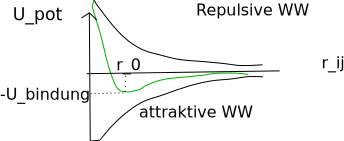
\includegraphics{figures/1_1graph}
	\end{center}
	Beispiel: $U_{pot}^{ij}(r_{ij})= \frac{-a}{r_{ig}^m}+\frac{b}{r_{ij}^n}$ mit $a,b,n,m > 0$ und $n>m$ \newline
	Bindungsenergie:
	\begin{align}
		U_{Bindung} = \frac{1}{2}\sum_i\sum_{i\neq j}U_{pot}(r_0) = \frac{N}{2} \sum_{i\neq j} U_{pot}(r_0)
	\end{align}
	Abschätzung: Coulomb-WW von 2 Ionen $|q| = e$, und $r_0 = 1nm$
	\begin{align}
		U_{pot} \approx \frac{e^2}{4\pi\epsilon\cdot e_0}=\SI{1.4}{\electronvolt} \rightarrow U_{Bindungen} \approx U_{pot} N_A = \SI{140}{\kilo\joule\per\mole}
	\end{align}

\paragraph{Diskussion}
	\begin{itemize}
		\item[1)] attraktive WW: Art der Bindung, vgl. nächste Unterkapitel
		\item[2)] repulsive WW: Atom-Wellenfunktionen dürfen sich nicht vollständig durchdringen aufgrund des Pauli-Prinzips. phänomenologisch: $U_{rep}(r)\approx \frac{1}{r^{12}}$(also n=12)
		\item[3)] NB: Alternative Ansätze: $\approx \frac{1}{r^2}$ mit $6<n<10$
	\end{itemize}

\paragraph{Bindungstypen}
	5 Typen, abhängig von der Elektronenkonfiguration
	\begin{itemize}
		\item[I] \textbf{Van-Der-Waals Bindung:}\newline
			abgeschossene äußere Schale \newline
			Dipol-WW, sehr schwach (0.1eV)\newline
			zum Beispiel Edelgaskristall
		\item[II] \textbf{Ionenbindung:} \newline
			Elektronentransfer $\rightarrow$ Edelgaskonfiguration \newline
			Coulomb-WW, stark (10eV) \newline
			zum Beispiel: NaCl
		\item[III] \textbf{Kovalente Bindung}:\newline
			Überlapp der Elektronenhülle $\rightarrow$  Überlapp der Wellenfunktionen der Valenzelektronen\newline
			$\rightarrow$ gerichtete Bindung \newline
			Coulomb-WW, gerichtet, stark (10eV)\newline
			zum Beispiel Diamant, Silizium
			\begin{center}
				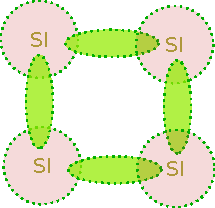
\includegraphics{figures/1_1silizium.pdf}
			\end{center}
		\item[IV] \textbf{metallische Bindung}\newline
			Valenzelektronen komplett delokalisiert, es entsteht \glqq freies Elektronengas\grqq{}
			um die Ionenrümpfe \\
			Coulomb-WW, eher schwach (1eV)\\
			zum Beispiel Na
		\item[V] \textbf{Wasserstoff-Brückenbindung}\newline
			Bindung über ein H-Atom, dass Bindung vermittelt.\newline
			Coulomb-WW, schwach
			\begin{center}
				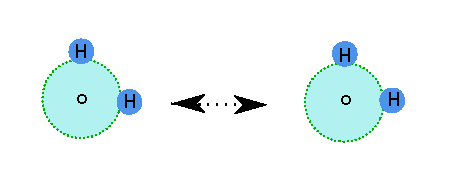
\includegraphics{figures/1_1wasserstoff.pdf}
			\end{center}
			organische Substanzen: DNA Doppelstrang
	\end{itemize}

\subsection{Van-Der-Waals Bindung}\label{kap:1_2}
	Betrachte Atome eines Edelgases mit vollständig besetzten s-und-p-Schalen.
	\begin{itemize}
		\item Kugelsymmetrische Ladungsverteilung
		\item Bindung durch Fluktuationen dieser Ladungsteilungen um den Kern.
		\item Klassische Beschreibung:
			\begin{enumerate}
				\item Verschiebung der Ladungsverteilung in Atomen 1 $\rightarrow$ Dipolmoment $p_1$
				\item Dipol $p_1$ erzeugt elektrisches Feld $E_1$\newline
						Atom 2 im Abstand $r$ von Atom 1:
						\begin{align}
							E_1(r)=\frac{1}{4\pi\epsilon_0}\left(3\frac{p_i r}{r^5}r-\frac{1}{r^3}p_1\right) \
							E_1(r) \propto \frac{p_1}{r^3}
						\end{align}
				\item Atom 2 wird von $E_1$ auch Polarisiert.
						\begin{align}
							P_2 \propto E_1(r) \text{mit Polarisierbarkeit}
							p_2 \propto \frac{p_1}{r^3}
						\end{align}
				\item Elektrisches Feld von Atom 2 am Ort von Atom 1:
						\begin{align*}
							E_2(r) = \frac{1}{4\pi\epsilon_0}\left(3\frac{P_2}{\vec{r}^5}\vec{r}-\frac{1}{\vec{r}^3}p_2\right)
						\end{align*}
				\item Gegenseitige Beeinflussung der Atome stört die kugelsymmetrische Ladungsteilungen, so dass $<p_1>^2 \neq 0$.
				\item Wechselwirkung: $U_{pot}^{12}(r)= -p_2\cdot E_1(r)\propto - \frac{1}{r^6}$
			\end{enumerate}
	\end{itemize}
	Damit: Paarpotential zweier Edelgasatome: \textbf{Lennard-Jones-Potential}
	\begin{align*}
		U_{pot}^{12}=\frac{A}{r^{12}}-\frac{B}{r^6} = e\epsilon\left[\left(\frac{\sigma}{r}\right)^{12} - \left(\frac{\sigma}{r}\right)^{6}\right]
	\end{align*}
	\begin{center}
		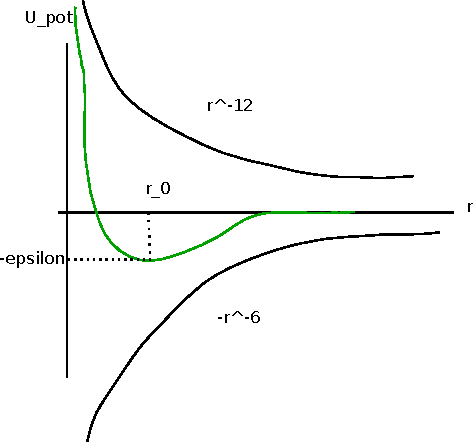
\includegraphics{figures/1_2graph.pdf}
	\end{center}
	mit $\epsilon = \frac{B^2}{4A}$ und $\sigma = \left(\frac{A}{B}\right)^{1/6}$\newline
	und $r_0 = 2^{1/6}\sigma=1.12\sigma$\newline
	Gesamtes WW-Potential des Edelgaskristalls:
	\begin{itemize}
		\item Summation über alle Atome, vgl. Gl 1
		\item Potentialminimum: Gitterabstand $R_0 (\neq r_0)$
	\end{itemize}
	Vergleich: Abschätzung-Experiment:
	\begin{table}[h]
		\centering
		\begin{tabular}{l|llll}
													& Ne & Ar & Kr  & Xe  \\ \hline
			$U_{bidung}^{exp}$ in $\frac{meV}{Atom}$ & 20 & 81 & 116 & 166 \\
			$U_{bidung}$                             & 26 & 89 & 127 & 174 \\
			Korrektur Nullpunktsfluktuation          & -8 & -9 & -7  & -6  \\
			$\sum$                                   & 18 & 80 & 120 & 168
		\end{tabular}
	\end{table}\\
	Was fehlt? Nullpunktsfluktuationen als Unschärferelation $\Delta x\cdot \Delta p \geq \frac{\hbar}{2}$\newline
	Trick: Annäherung von L-J-Pot. nahe $R_0$ durch harmonischen Oszillator \newline
	$\rightarrow \Delta x = \sqrt{\frac{h}{2m\omega}}$

\subsection{Ionische Bindung} \label{kap:1_3}
	Betrachte Atome, die durch Austauch von Elektronen die Edelgaskonfiguration erreichen können.\\
	Bsp.: NaCl
	\begin{itemize}
		\item Na: $1$s$^2 2$s$^2 2$p$^6 3$s$^1 \rightarrow \, \text{Na}^+: \, 1$s$^2 2$s$^2 2$p$^6$
		\item Cl: $1$s$^2 2$s$^2 2$p$^6 3$s$^2 3$p$^5 \rightarrow \, \text{Cl}^-: \, 1$s$^2 2$s$^2 2$p$^6 3$s$^2 3$p$^6$
	\end{itemize}
	\begin{itemize}
		\item[$\rightarrow$] Ionen haben Kugelsymmetrische Ladungsverteilung
		\item[$\rightarrow$] Coulomb-WW (ungerichtet)\\
			Abschätzung: 2 Ionen mit $q = \pm e$ im Abstand $a = 2.8$ \AA:\\ $U_{Coulomb} = -\frac{e^2}{4 \pi \varepsilon_0 a} = - 8.2 \cdot 10^{-19} \text{J} = -5.1 \text{eV}$
	\end{itemize}

	Coulomb-WW ist deutlich stärker als van-der-Waals-WW \\
	(Auch Nullpunktsfunktionen können vernachlässigt werden)\\
	$\rightarrow$ WW im Kristall ist durch WW mit vielen Nachbarionen stärker als die Anschätzung.

\paragraph{Bindungsenergie im Ionenkristall:}
	Verwende 1 aus Kap. \ref{kap:1_1}
	\begin{align*}
		\Phi_i  = \sum_{j \neq i} \left(\pm \frac{Z^2 e^2}{4 \pi \varepsilon_0 r_{ij}} + \frac{A}{r_{ij}^{12}}\right)
	\end{align*}

	Ann: Abstoßende WW ist kurzriechweitig, d.h. nur nächste Nachbarn im Abstand R. Die Zahl der Nächsten Nachbarn $n$ hängt von der Struktur ab.
	\begin{align*}
		\Phi_i                                   & = \sum_{j \neq i} \left(\pm \frac{Z^2 e^2}{4 \pi \varepsilon_0 r_{ij}} + n\frac{A}{R^{12}}\right)
		\qquad \text{mit } r_{ij} = p_{ij} \cdot R                                                                                                                 \\
												& = - \frac{Z^2 e^2}{4 \pi \varepsilon_0 R} \left(\sum_{j \neq i} \frac{\pm 1}{p_{ij}}\right) + n\frac{A}{R^{12}} \\
		\text{Madelung-konstante:} \qquad \alpha & := \left(\sum_{j \neq i} \frac{\pm 1}{p_{ij}}\right)
	\end{align*}
	VZ: +: unterschidliche Ladung; -: gleiches VZ der Ladung.\\
	$\alpha$ hängt von der Kristallstruktur ab. Für NaCl:
	\begin{figure}
		\centering
		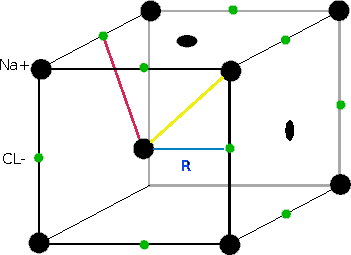
\includegraphics{figures/1_3NaCl.pdf}
		\caption{Vgl. Kap. 2: fcc-Gitter mit 2-atomiger Basis}
	\end{figure}
	jeder Baustein:
	\begin{itemize}
		\item 6 Nachbarn mit $p_{ij} =  1$
		\item 12 Nachbarn mit $p_{ij} =  \sqrt{2}$
		\item 8 Nachbarn mit $p_{ij} =  \sqrt{3}$
	\end{itemize}

	Damit:
	\begin{align}
		\alpha = +6 \cdot \frac{1}{1} - 12 \cdot \frac{1}{\sqrt{2}} + 8 \cdot \frac{1}{\sqrt{3}} - \dots
	\end{align}
	Problem: Reihe ist nur bedingt konvergent. Physikalisch: Oberflächenladung.\\
	Trick: \textbf{Evjen-Methode:} Zerlegung des Kristalls in Zellen mit der Symmetrie des Kristalls, die elektrisch ungeladen sind.
	$\Rightarrow$ Anteilige Zählung von Ladungen an Stirnflächen ($\frac{1}{2}Z$), Kanten ($\frac{1}{4}Z$), Ecken ($\frac{1}{8}Z$).\\
	$\rightarrow$ Für die kleinste Zelle:
	\begin{align}
		\alpha_1 = 6 \cdot \frac{1}{2} \cdot \frac{1}{1}  - 12 \cdot \frac{1}{4} \cdot \frac{1}{\sqrt{2}} + 8 \cdot \frac{1}{8} \cdot \frac{1}{\sqrt{3}} \approx 1.45
	\end{align}
	Madelung-Konstante durch Summation
	\begin{align*}
		\alpha_{NaCl} = \alpha_1 + \alpha_2 + \dots \approx 1.748
	\end{align*}

	Bindungsenergie pro Ionepaar $\Phi_i$
	Gesamte Bindungsenergie: 
	\begin{align} 
		\Phi = \frac{1}{2} \sum_i \Phi_i = \frac{N}{2} \cdot \Phi_i (\text{vgl. Gl. (1)})  \\
		\text{für }\frac{N}{2}\text{ Ionenpaare} \nonumber
	\end{align}
	Gleichgewitszustand $R_0$:
	\begin{align*}
		\frac{\mathrm{d} \varphi}{\mathrm{d} R} = 0 \qquad \text{(Minimierung der pot. Energie)} \\
		\rightarrow \qquad U_{Bindung} = \Phi (R_0) = - \frac{N \alpha Z^2 e^2}{8 \pi \varepsilon_0 R_0} \left(1- \frac{1}{12} \right)
	\end{align*}

	für NaCl: $R_0$ = 2.8 \AA\\
	$U_{Bindung, pro Ionenpaar} = 8.23$ eV\\
	$U_{Bindung,p.I.}^{exp} = 7.95$ eV \\

\paragraph{Chemisch Interpretation der Bindungsenergie:}
	$U_{Bindung} =$ Energie, die Bei Zerlegung des Kristalls in Bausteine aufgewendet werden muß:
	\begin{align*}
		\text{NaCl} \rightarrow \text{Na}^+ + \text{Cl}^-
	\end{align*}
	weiter Energien:
	\begin{itemize}
		\item Ionisierungsenerige des Na $\rightarrow$ Na$^+$ + e$^-$ (5.14 eV)
		\item Elektronenaffinität des Cl + e$^-$ $\rightarrow$ Cl$^-$ (-3.61 eV)
		\item Dissotiation von Cl$_2$ $\rightarrow$ 2Cl
		\item Sublimation von Na-Atomen aus Na-Kristall
	\end{itemize}
(Haber-Born-Kreisprozess)

\subsection{Kovalente Bindung} \label{kap:1_4} %1.4
Betrachte Atome, deren Wellenfunktionen überlappen:
\begin{itemize}
	\item[$\rightarrow$] Entstehung von (Molekül-) Orbitalen, durch die die elektron. Wellenfunktion zwischen den Partnern lokalisiert wird.
	\item[$\rightarrow$] Stark gerichtet, kurzreichweitig, stark
	\item[$\rightarrow$] Moleküle (H$_2$, CH$_4$,\dots), Festkörperphysik (Diamant, Silizium)
	\item[$\rightarrow$] vdW-WW spielt auch in kovalenten Kristallen keine Rolle. 
\end{itemize}
\paragraph{Bestimmung der Bindungsenergie}
$\rightarrow$ IK4, Kap. 17
\paragraph{Bindungsenergie}
Beispiel: \textbf{H$_2^+$-Molekül-Ion}
\begin{figure}[H]
	\centering
	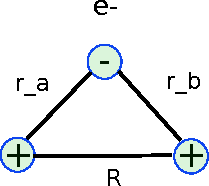
\includegraphics{figures/1_4WasserstoffH2O.pdf}
	\caption{}
	\label{}
\end{figure}
\textbf{Näherungsmethode}: LCAO-Methode (linear combination of atomic orbitals)
\begin{itemize}
	\item Hamilton-Operator: $\hat H = - \frac{\hbar^2}{2m} \Delta - \frac{e^2}{4 \pi \varepsilon_0 r_a} - \frac{e^2}{4 \pi \varepsilon_0 r_b} +\frac{e^2}{4 \pi \varepsilon_0 R}$
	\item SGL: $\hat H \vert\Psi\rangle = E \vert\Psi\rangle$
	\item $\Psi$: Annahme: Für große R hält sich $e^-$ bei Proton a oder b auf und seine Grundzustands-Wellenfunktion ist $\vert\Psi_a\rangle$ oder $\vert\Psi_b\rangle$.\\
\end{itemize}
Für kleinere Abstände R sei $\vert\Psi\rangle = c_1 \vert\Psi_a\rangle + c_2 \vert\Psi_b\rangle$. \\
Damit:
\begin{align*}
	E &= \frac{\langle\Psi\vert\hat{H}\vert\Psi\rangle}{\langle\Psi\vert\Psi\rangle} = \frac{c_1^2 H_{aa} + c_2^2 H_{bb} + 2 c_1 c_2 H_{ab}}{c_1^2 + c_2^2 + 2 c_1 c_2 S}\\
	\text{mit } H_{aa,bb} &= \langle\Psi_{a,b}\vert\hat{H}\Psi_{a,b}\vert\rangle\\  
	H_{ab} &= \langle\Psi_a\vert\hat{H}\vert\Psi_a\rangle = H_{ba}
\end{align*}
Minimierung von $E$ bzgl. $c_1$ und $c_2$:
\begin{align*}
	\frac{\partial E}{\partial c_1} &\stackrel{!}{=} 0 \stackrel{!}{=} \frac{\partial E}{\partial c_2}\\
	\Rightarrow \quad &c_1(H_{aa}-E)+c_2(H_{ab}-E\cdot S) \stackrel{!}{=} 0\\
	&c_1(H_{ab}-E\cdot S)+c_2(H_{bb}-E) \stackrel{!}{=} 0
\end{align*}
\begin{itemize}
	\item[$\rightarrow$] Koeffizientendeterminante verschwindet, falls:
	$$ (H_{aa}-E)(H_{bb}-E) - (H_{ab}-E \cdot S)^2 \stackrel{!}{=} 0 $$
	\item[$\rightarrow$] Mit $H_{aa} = H_{bb}$ : $c_1 = \pm c_2 $
	$$E_{\pm} = \frac{H_{aa} \pm H_{ab}}{1 \pm S} \quad \text{und} \quad \vert\Phi_{\pm}\rangle = c (\vert\Psi_a\rangle \pm \vert\Psi_b\rangle) $$
\end{itemize}
\paragraph{Interpretation}

\begin{figure}[H]
	\centering
	\includegraphics{figures/1_4graph.pdf}
	\caption{}
	\label{}
\end{figure}

\begin{figure}[H]
	\centering
	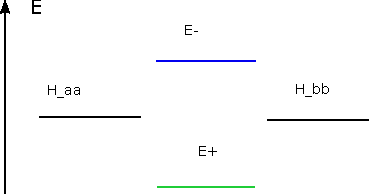
\includegraphics{figures/1_4Energie.pdf}
	\caption{$\rightarrow E_-$ liegt energetisch höher (Antibindendes Orbital \textbf{blau}, bindendes Orbital \textbf{grün})}
	\label{}
\end{figure}
\begin{itemize}
	\item[$\rightarrow$] $\vert\Psi_+\rangle$ ist symmetrisch, d.h. $|\Psi_+|^2$ ist zwischen $a$ und $b$ erhöht.
	\item[$\rightarrow$] $\vert\Psi_-\rangle$ ist antisymmetrisch, d.h. $|\Psi_-|^2$ hat eine Nullstelle zwischen $a$ und $b$.
	\item[$\rightarrow$] $E_+$ ist energetisch günstiger, denn $|\Psi_+|^2$ zwischen $a$, $b$ erhöht $\rightarrow$ Abschwächung der Coulomb-Abstoßung von $a$ und $b$.
\end{itemize}

Systeme mit mehr als 1 Valenzelektron:
\begin{itemize}
	\item zusätzliche Coulomb-Abstoßung der Elektronen
	\item \textbf{Pauli-Prinzip:} Fermionen haben antisymmetrische Gesamt-Wellenfunktion.
	\begin{itemize}
		\item symmetrische Ortswellenfunktion $\vert\Psi\rangle$ und antisymmetrische Spin-Wellenfunktion (Singulett)
		\item antisymmetrische Ortswellenfunktion $\vert\Psi\rangle$ und symmetrische Spin-Wellenfunktion (Triplett)
	\end{itemize}
\end{itemize}
\begin{figure}[]
	\centering
	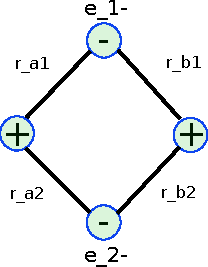
\includegraphics{figures/1_4H2Moleuel.pdf}
	\caption{}
	\label{}
\end{figure}

\textbf{Näherungsmethode}: Heitler-London-Methode\\
Vorgehen analog zu LCAO-Methode, aber mit Zweiteilchen-Welenfunktion.\\
Allgemein Symmetrische/Antisymmetrische Ortswellenfunktion
\begin{align*}
	\Psi_s(\textbf{r}_1,\textbf{r}_2) &\sim (\Psi_a(\textbf{r}_1) + \Psi_b(\textbf{r}_1)) (\Psi_a(\textbf{r}_2) + \Psi_b (\textbf{r}_2))\\
	\Psi_a(\textbf{r}_1,\textbf{r}_2) &\sim (\Psi_a(\textbf{r}_1) - \Psi_b(\textbf{r}_1)) (\Psi_a(\textbf{r}_2) - \Psi_b (\textbf{r}_2))
\end{align*}
Annahme:
\begin{align*}
	\Psi_{s,a}(\textbf{r}_1,\textbf{r}_2) \sim \Psi_a(\textbf{r}_1) \Psi_b (\textbf{r}_2) \pm \Psi_b (\textbf{r}_1) \Psi_a (\textbf{r}_2)
\end{align*}
weiteres Vorgehen analog.
Diskussion:
\begin{itemize}
	\item Lovalente Bindungen nur bei starkem Überlapp der Wellenfunktionen.
	\item Höchstens 2 Elektronen, damit nur bindendes Molekülorbital besetzt wird.
	\item Ortsabhängigkeit der Wellenfunktion $\rightarrow$ Kovalente Bindung nur in bestimten Richtungen im Kristall
\end{itemize}

\textbf{Allgemeiner Ansatz:} Zweiteilchen-Ortswellenfunktion
\begin{align*}
	\Psi_s(\textbf{r}_1,\textbf{r}_2) = \Psi_s(\textbf{r}_1) \Psi_s(\textbf{r}_2) &\sim (\Psi_a(\textbf{r}_1) + \Psi_b(\textbf{r}_1)) (\Psi_a(\textbf{r}_2) + \Psi_b (\textbf{r}_2))\\
	\Psi_a(\textbf{r}_1,\textbf{r}_2) = \Psi_s(\textbf{r}_1) \Psi_A(\textbf{r}_2) &\sim (\Psi_a(\textbf{r}_1) + \Psi_b(\textbf{r}_1)) (\Psi_a(\textbf{r}_2) - \Psi_b (\textbf{r}_2))
\end{align*}

\paragraph{Wichtige Fälle}
\begin{itemize}
	\item[(a)] \textbf{sp$^3$-Hybridisierung: z.B. Diamant}\\
	C: $1$s$^2 \, 2$s$^2 \, 2$p$^2$ $\rightarrow$ 2 kovalente Bindungen?\\
	\begin{itemize}
		\item[$\rightarrow$] Rehybridisierung: größere Bindungsenergie durch 4 kovalente Bindungen. Zerlegung von $2$s$^22$p$^2$ in $2$s$^12$p$_x^12$p$_y^12$p$_z^1$\\
		Bildung von Linearkombinationen (sp$^3$-Orbitale):\\
		$$\Psi_i = \frac{1}{2} (\Psi_S \pm \Psi_{p_x} \pm \Psi_{p_y} \pm \Psi_{p_z}) \quad \text{mit} \quad (+++), (+--), (-+-), (--+)$$
		\item [$\rightarrow$] 4 tetraedisch angeordnete Keulen\\
		\begin{figure}[H]
			\centering
			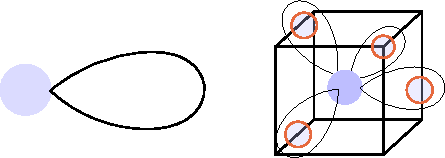
\includegraphics{figures/1_4bindungen.pdf}
			\caption{sp$^3$-Orbital (links) und 4sp$^3$-Orbitale (rechts). Winkel der Kugelwolken $109,5$ deg }
			\label{}
		\end{figure}
		\item[$\rightarrow$] Tetraederstruktur (sp$^3$-Hybridisierung): viele Materialien, z.B. Si, Ge, GaAs,...
	\end{itemize}
	\item[(b)] \textbf{sp$^3$-Hybridisierung}, z.B. Graphen\\
	C:  $1$s$^2 \, 2$s$^2 \, 2$p$^2$\\
	\begin{itemize}
		\begin{figure}[H]
			\centering
			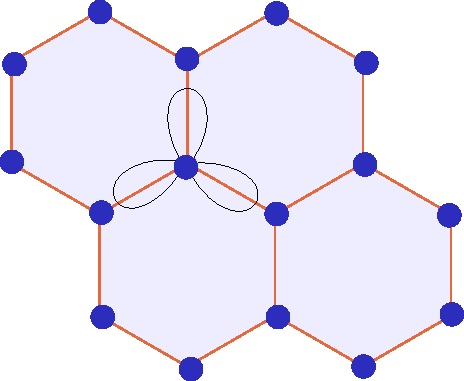
\includegraphics{figures/1_4Kristall.pdf}
			\caption{Winkel 120 deg}
			\label{}
		\end{figure}
		\item[$\rightarrow$] Rehybridisierung: sp$^3$-Orbitale \\
		$2$s$^1$ 2p$_x^1$ 2p$_y^1$ \\ 
		Das übrige 2p$_z$ $\bot$ sp$^2$-Ebene kann $\pi$-Bindungen eingehen (delokalisierte Elektronen), z.B. für Bindungen Graphit $\rightarrow$ Graphit. 
	\end{itemize}
\end{itemize}

\subsection{Metallische Bindung} %1_5
\label{kap:1_5}
\begin{itemize}
	\item[$\rightarrow$] Überlapp von elektronischen Wellenfunktionen, allerdings hier mit vielen Atomen
	\item[$\rightarrow$] Es entsteht ein sogenanntes \textit{freies Elektronengas}, d.h. Valenzelektronen sind delokalisiert.
	\item[$\rightarrow$] Bindung ist ungerichtet und nicht so stark, wie die kovalente Bindung, wg. Abschirmung durch Rümpfe:
	\begin{table}[H]
		\centering
		\begin{tabular}{l|l|l|l|l}
						 & Li   & Na   & Fe   & Co   \\
						 \hline
		$U_{Bidung}$(eV) & 1,63 & 1,11 & 4,28 & 4,39 \\    
		\end{tabular}
		\end{table}
	\textbf{NB:} Übergangsmetalle (d-Elektronen)  haben kovalenten Anteil und daher stärkere Bindungsenergie.
	\item[$\rightarrow$] relativ geringe $U_{Bindung}$ $\rightarrow$ Gitterabstände größer als bei kovalenten o. Ionenkristallen.\\
	$\rightarrow$ Metalle weich, kl.Schmelztemperatur
	\item[$\rightarrow$] hohe elektrische und thermische Leitfähigkeit durch \textit{freie} Valenzelektronen.
\end{itemize}
[Details: erfordern elektronische Eigenschaften von Kristallen]

\subsection{Wasserstoff-Brückenbindung} %1_6
\label{kap:1_6}
Bindung eines H-Atoms an 2 andere Atome, die nicht in \ref{kap:1_2}, \ref{kap:1_3}, \ref{kap:1_4}, \ref{kap:1_5}%TODO: make labels in the according kap's%
passt.\\
$\rightarrow$ H: 1s$^1$ d.h Ionenbindung grundsätzlich möglich, aber $U_{Bindung}$ = 13.6 eV zu stark, genauso für metallische Bindung. Kovalente Bindung möglich. \\
$\rightarrow$ Bindungspartner mit hoher Elektronegativität (z.B. O, N, F): H-Brücke.
\begin{figure}[H]
	\centering
	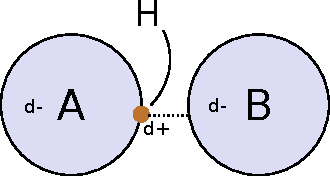
\includegraphics{figures/1_6Wasserstoff.pdf}
	\caption{Valenzelektron des H-Atoms geht fast vollständig auf Bindungspartner A über.\\
	Effektive positive Ladung $\rightarrow$ Bindung an B.\\
	Keine weiteren Bindungspartner aus räumlichen Gründen.}
	$U_{Bindung pro Atom}$ = 0.1 eV (ähnlich wie VDW-Bindung)
	\label{}
\end{figure}

$\rightarrow$ thermische Aktivierung bei Raumtemperatur $\rightarrow$ Biomoleküle\\
typischer Bindungsabstand: 1-2 \AA (also $>>$ vdW-Bindung)\\
z.B. H$_2$O ($\rightsquigarrow$ Dichteanomalie), DNA Doppelhelix

\section{Kristallstrukturen} \label{kap:2}
Hier: idealen Kristallen, also unendlich Wiederholungen von identischen Strukturen (keine Oberfläche, Defekte, \dots)
\begin{itemize}
    \item Bekante Atomsorte(n) und Bindgunsart: wohldefinierte Gleichgewichtslängen.
    \item Gesamtenergie des Kristalls ist minimal, wenn alle Bausteine genau dieselbe Umgebung vorfinden
    \item \textbf{Struktur} Beschreibung als \textbf{Basis} (Strukturelement) + \textbf{Gitter} (Bauplan, Aneinanderziehung der Strukturelemente)
          \begin{itemize}
              \item Basis: 1 Atom (Au), 2 Atome (Diamant, Si, NaCl, GaAs), \dots, 13 Atome (YBa$_2$Cu$_3$O$_7$), \dots $>10^4$ Atome in Proteinkristallen
              \item Gitter: In 3D nur 14 Bravais-Gitter
          \end{itemize}
\end{itemize}

\subsection{Kristallgitter} \label{kap:2_1}
\textbf{Def.:} Unendlich große, regelmäßige, periodische Anordnung von Raumpunkten. Es sieht immer gleich aus, unabhängig von welchem Gitterpunkt es betrachtet wird.\\
Das Kristallgitter wird durch die \textbf{fundamentalen Gittervektoren} \textbf{a$_1$}, \textbf{a$_2$}, \textbf{a$_3$} aufgespannt, d.h. jeder Gitterpunkt durch $\textbf{R} = n_1 \textbf{a}_1 + n_2 \textbf{a}_2 +n_3 \textbf{a}_3$ ($n_1$, $n_2$, $n_3$ ganzzahlig) beschrieben. Die Länge der fundamentalen Gittervektoren definieren die sog. \textbf{Gitterkonstante}.\\
\textbf{Primitive Gittervektoren} erreichen (bei vorgegebenem Ursprung) alle Gitterpunkte.\\
Die (primitiven) GV \textbf{a$_1$}, \textbf{a$_2$}, \textbf{a$_3$}, spannen Parallelepiped auf. Dieses stellt die (primitiven) \textbf{Elementarzelle} dar.\\
\begin{itemize}
    \item Die primitive Elementarzelle enthält genau 1 Gitterpunkt und ist die kleinstmögliche Elementarzelle
    \item Die primitive Elementarzelle ist nicht eindeutig definiert. Alle möglichen primitiven EZ haben dasselbe Volumen $V = \textbf{a}_1 (\textbf{a}_2 \times \textbf{a}_3)$ (Spatprudukt)
    \item Die primitive EZ muss nicht zwingend die Symmetrie des Gitters widerspiegeln. Die kleinstmögliche EZ, die die volle Gittersymmetrie hat, ist die \textbf{konventionelle EZ} (vgl. Folie 3 rechts)
\end{itemize}
\paragraph{Wigner-Seitz-Zelle}
\begin{figure}[H]
    \centering
    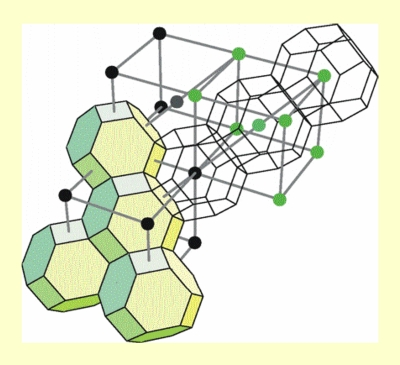
\includegraphics[width=0.4\textwidth]{figures/2_1wignerseitz.jpg}
    \caption{Wigner-Seitz Zelle}
    \label{}
\end{figure}
\begin{itemize}
    \item primitive EZ, die die volle Symmetrie des Gitters wiederspiegelt
    \item Sie erhält den Teil des Raumes um einen Gitterpunkt der diesen näher ist als die übrigen Gitterpunkte
    \item Konstruktionsvorschrift:
          \begin{itemize}
              \item[1.] Verbindungslinien von Gitterpunkt zu Nachbarn (Folie 4, grün gestrichelt)
              \item[2.] Mittelsenkrechte (Mittelebene, 3D) auf diesen Linien
              \item[3.] Wigner-Seitz-Zelle ist die kleinste eingeschlossene Fläche/Volumen
          \end{itemize}
\end{itemize}
\begin{figure}[H]
    \centering
    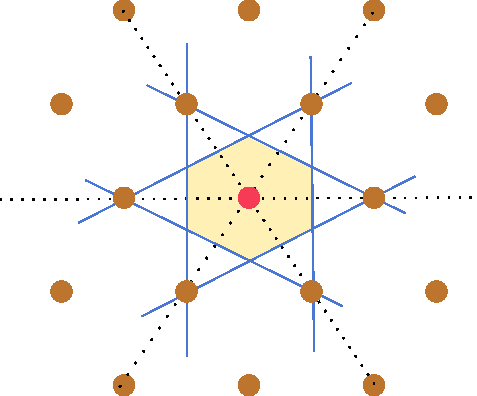
\includegraphics{figures/2_1Gitter.pdf}
    \caption{Beispiel}
    \label{}
\end{figure}
\paragraph{Symmetrien:}
\begin{itemize}
    \item[(a)] Translationssymmetrie:\\
          Kristallgitter ist invariant unter Transformation mit Translationsvektor $\textbf{T} = n_1 \textbf{a}_1 + n_2 \textbf{a}_2 +n_3 \textbf{a}_3$ ($n_1$, $n_2$, $n_3$ ganzzahlig)
          \begin{itemize}
              \item[$\rightarrow$] Für jeden Punkt \textbf{r} mit Umgebung $\mathcal{U} (\textbf{r})$: identische Umgebung am Ort \textbf{r} + \textbf{T}, also $\mathcal{U} (\textbf{r} + \textbf{T}) = \mathcal{U} (\textbf{r})$
              \item[$\rightarrow$] Durch Translation der primitiven EZ lässt sich der Raum lückenlos und ohne Überöappauffüllen.
              \item[$\rightarrow$] Durch Translation um die primitiven GV lässt sich jeder Gitterpunkt erreichen.
          \end{itemize}
          {figure}\begin{figure}[H]
            \centering
            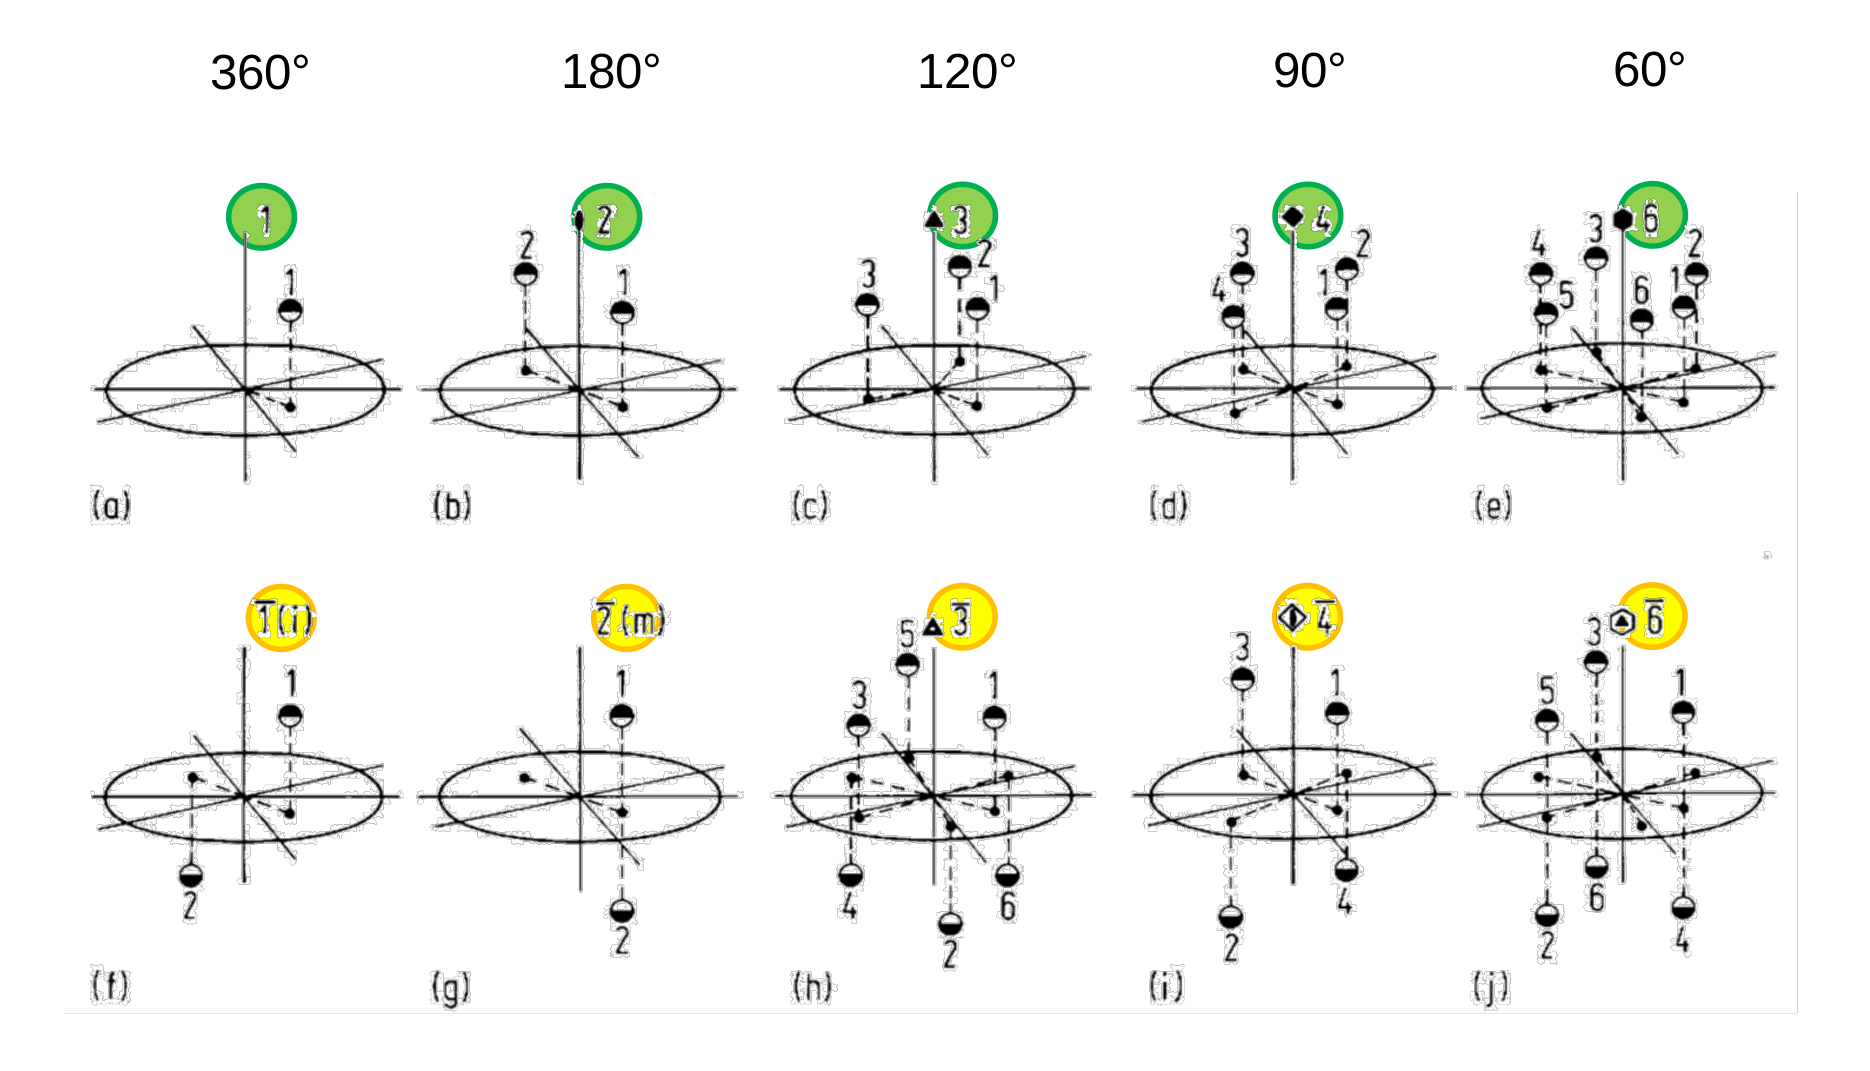
\includegraphics[width=\textwidth]{figures/2_1Symmetrie}
            \caption{Symmetrieoperationen der Punktgruppe}
            \label{}
        \end{figure}
    \item[(b)] Punktsymmetrie-Operationen:\\
          Unter Punktsymmetrie-Operationen bleibt mindestens 1 Punkt im Raum unverändert
          \begin{itemize}
              \item[(i)] \textbf{Drehung um eine Drehachse:}\\
                    Drehung, unter denen das Gitter invariant ist:
                    \begin{table}[H]
                        \centering
                        \begin{tabular}{l|lllll}
                            Winkel in rad             & $2 \pi$ & $\frac{2\pi}{2}$ & $\frac{2\pi}{3}$ & $\frac{2\pi}{4}$ & $\frac{2\pi}{6}$ \\\hline
                            Zähligkeit der Drehachsen & 1       & 2                & 3                & 4                & 6
                        \end{tabular}
                    \end{table}
                    \textbf{NB:} Es gibt kein Kristallgitter mit Zähligkeit $>6$. Es gibt kein Kristallgittermit 5-zähliger Symmetrie. Diese ist kompatibel mit Translationssymmetrie. Quasikristalle haben 5-zählige Symmetrie, sind aber nicht periodisch.
              \item[(ii)] \textbf{Spiegelung:} $x  \rightarrow  -x$, $y  \rightarrow y$, $z  \rightarrow  z$; Symbol: m
              \item[(iii)] \textbf{Inversion:} $x  \rightarrow  -x$, $y  \rightarrow -y$, $z  \rightarrow  -z$; Symbol: i oder 1\\
                    (Rotation um $\frac{2 \pi}{2} +$ Spiegelung an Ebene $\bot$ Drehachse)
              \item[(iv)] \textbf{Drehinversion} Drehung mit Zählgebiet 1,2,3,4,6,+ Inversionen; Symbol: z.B. $\overline{3} \rightsquigarrow $ 10 Symmetrieoperatoren der Punktgruppe.
          \end{itemize}
    \item[(c)] Klassifikation von Kristallgittern: \\
        Schema zur Einordnung von Kristallgittern nach ihren Symmetrieeigenschaften.
        \begin{itemize}
              \item[(I)] \textbf{Kristallsysteme}: \\ Gitterpunktgruppen, Symmetrie bzgl. Punktsymmetrie-Operationen.\\
              In 3D gibt es 7 Kristallsysteme:
              \begin{table}[H]
                \centering
                \begin{tabular}{l|llll}
                  Kristallsystem & Gitterkonstanten & Winkel & Zähligkeit & Anzahl\\\hline
                  triklin & $a_1 \neq a_2 \neq a_3$ & $\alpha \neq \beta \neq \gamma$ & 1 &  \\
                  monoklin & $a_1 \neq a_2 \neq a_3$ & $\alpha = \beta = 90^{\circ} \neq \gamma$ & 2 &  \\
                  orthorhombisch & $a_1 \neq a_2 \neq a_3$ & $\alpha = \beta = \gamma = 90^{\circ}$ & 2 &  \\
                  tetragonal & $a_1 = a_2 \neq a_3$ & $\alpha = \beta = \gamma = 90^{\circ}$ & 4 &  \\
                  hexagonal & $a_1 = a_2 \neq a_3$ & $\alpha = \beta = 90^{\circ}$; $\gamma = 120^{\circ}$ & 6 &  \\
                  trigonal & $a_1 = a_2 = a_3$ & $\alpha = \beta  = \gamma \neq 90^{\circ}$ & 3 &  \\
                  kubisch & $a_1 = a_2 = a_3$ & $\alpha = \beta = \gamma = 90^{\circ}$ & 3 &  \\
                \end{tabular}
            \end{table}
            Im FK treten häufig kubische oder hexagonale Kristallsysteme auf. Grund: Atome (Bausteine) sind $\approx$ Kugelsymmetrisch, daher Hochsymmetrie bevorzugt.
            \item[(II)] \textbf{Bravais-Gitter:}\\
            Gitter-Raumgruppe, Symmetrie bzgl. Punkt- und Translationsoperationen.
            \begin{figure}[H]
                \centering
                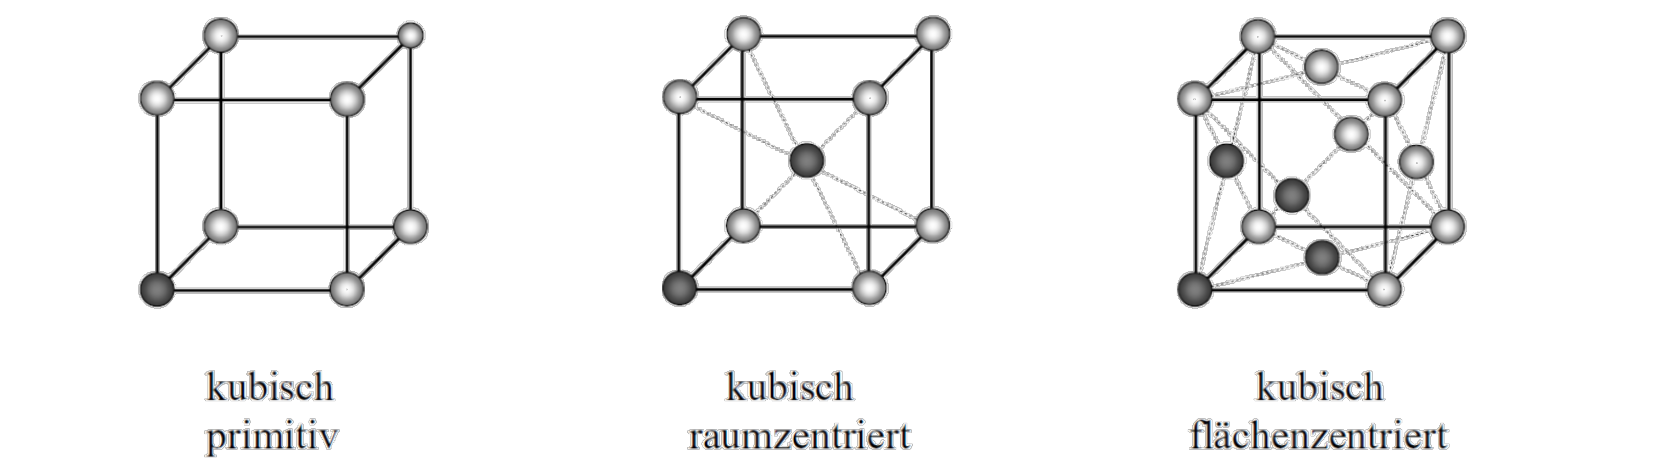
\includegraphics[width=0.7\textwidth]{figures/2_1KubischGitter}
                \caption{Beispiele für Bravais-Gitter}
            \end{figure}
            3D: 14 Bravais-Gitter
            \begin{itemize}
                \item So konstruiert, dass sie Symmetrie des Gitters widerspiegeln, dass sie also die höchste Zahl an Punktsymmetrie-Operationen enthalten.
                \item Nur 7 Bravais-Gitter haben primitive Elementarzelle.
            \end{itemize}
        \end{itemize}
\end{itemize}
\subsection{Einfluß der Basis} \label{kap:2_2}
Bisher: Nur Gitter. In 3D: 7 Kristallgitter (Gitter-Punktgruppen)\\
14 Bravisgitter (Gitter-Punktgruppen)\\
\begin{itemize}
    \item Beschreibung der Symmetrie Atomm $\rightarrow$ keine Änderung
    \item i.A. Basis Komplizierter:\\
    z.B kubisch primitives Gitter:
    \begin{figure}[H]
        \centering
        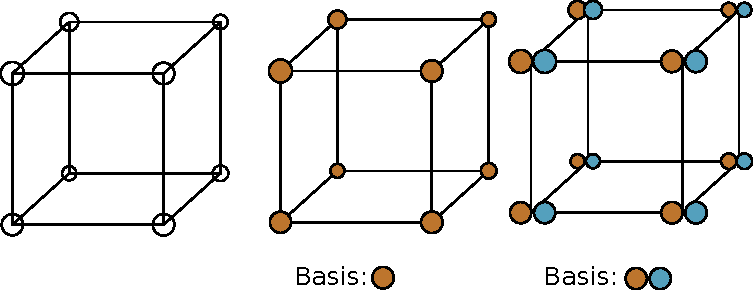
\includegraphics{figures/2_2Cubes.pdf}
        \caption{}
        \label{}
    \end{figure}
\end{itemize}
Analyze der Symmetrie des Kristalls (Gitter + Basis)\\
32 Kristallklassen (Punktgruppen)\\
230 Kristallophysische Raumgruppen (Raumgruppen)\\
\subsection{Beispiele einfacher Kristallstrukturen}
\label{kap:2_3}
Hier: Kristallstrukturen, die besonders häufig auftreten.
\begin{itemize}
    \item chemische Elemente:\\
    kubisch flächenzentriert (fcc): 21\\
    kubisch raumzentriert (bcc): 16\\
    hexagonal (hcp: hexagonal close packed): 33\\
    , aber: kubisch primitiv (sc = simple cubic): 1 ($\alpha$-Po)
    \item Weitere häufige Strukturen
    \begin{itemize}
        \item Diamant
        \item Zinkblende
        \item Kochsalz
        \item Cäsiumchlorid
    \end{itemize}
\end{itemize}
\begin{figure}[H]
    \centering
    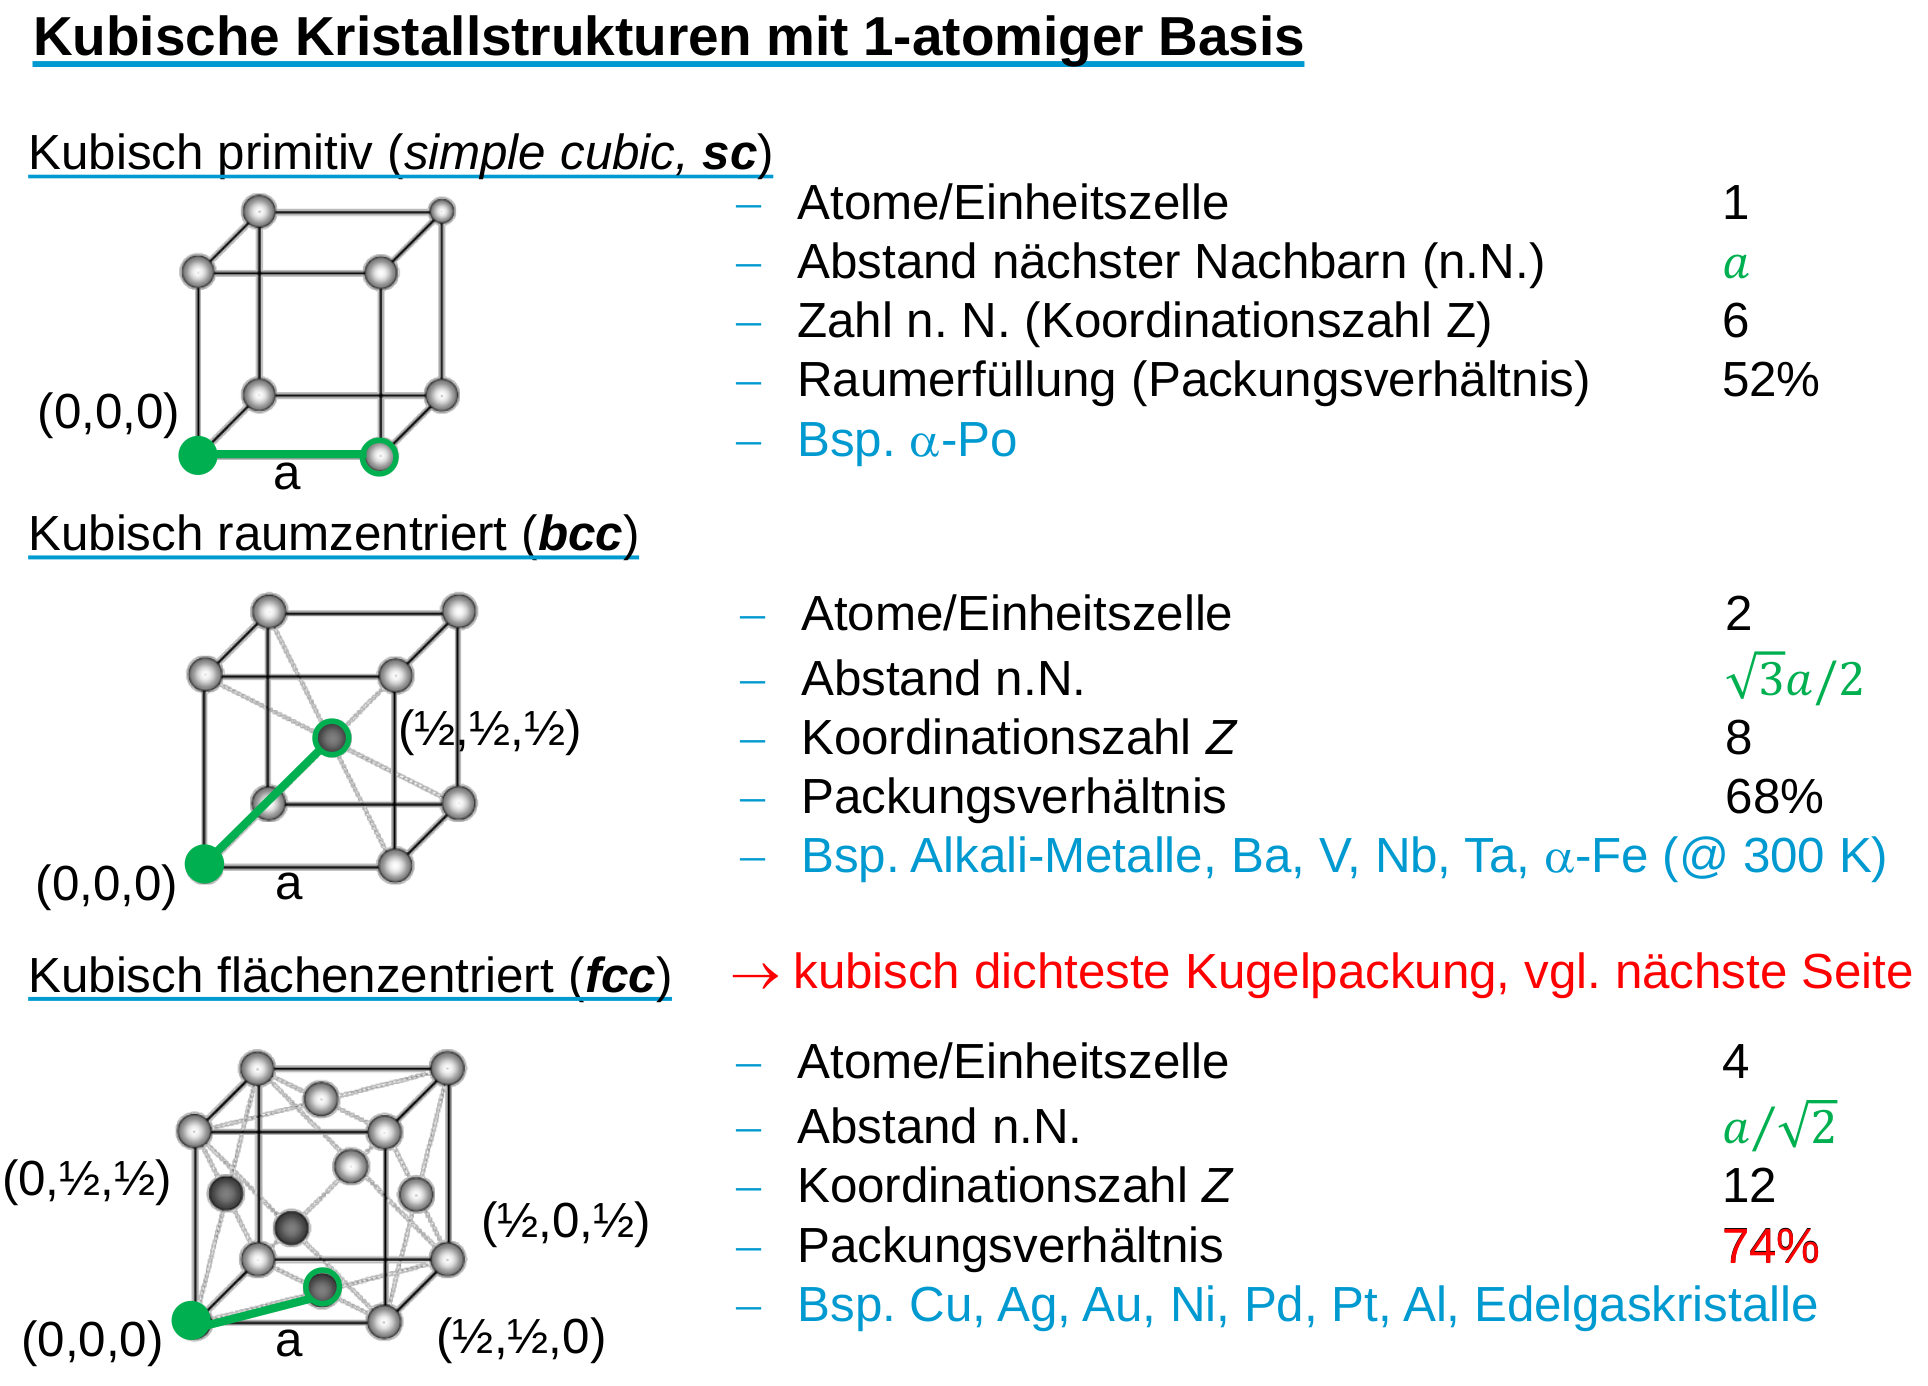
\includegraphics[width = \textwidth]{figures/2_2Kristallstrukturen1A.png}
    \caption{Vorlsungsfolie}
    \label{}
\end{figure}
\subsection{Indizierung von Kristllebenen und Richtungen}
\label{kap:2_4}
\textbf{Def:} Kristallebene (Gitterebene, Netzebene)
\begin{itemize}
    \item Ebene im Kristall, die durch Gitterpunkte aufgespannt wird.
    \item Tranlationsinvarianz des Kristalls: immer $\infty$ viele äquivalente Ebenen parallel zu jeder Kristallebene liegten.
    \item Festlegung durch Angabe der Durchstoßpunkte der Gitterachsen \textbf{a,b,c}
    \begin{figure}[H]
        \centering
        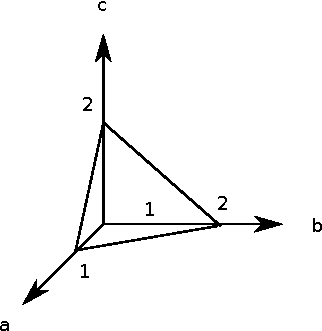
\includegraphics{figures/2_4dreieck.pdf}
        \caption{}
        \label{}
    \end{figure}
    \item Millerschen Indizes: Beziechnung von Kristallebenen Bestimmungsverfahren
    \begin{itemize}
        \item[(1)] Durchstoßpunkte in Einheriten der Gitterkonstante, z.B. 122
        \item[(2)] Kehrwert, z.B. $1, \frac{1}{2}, \frac{1}{2}$
        \item[(3)]  Multiplicationen mit kleinstmöglicher Faktoren, der geanzen Zahlen liefert (hier: 2) führt auf Millerschen Indizes hkl, z.B. 211
    \end{itemize}
    \begin{itemize}
        \item Sonderfälle:\\
        Kristallebene || Gittervektor $\rightarrow$ Schnittpunkt $\infty$, index 0
        \item Durchstoßpunkt auf negativer Achse: Notation $1$ oder $2$
    \end{itemize}
    \paragraph{Diskussion:}
    \begin{itemize}
        \item Miller Indizes hängen von der Wahl der Gittervektoren ab.
        \item (hkl) bezeichnet Schar von Ebenen, die parallel sind.
        \item [hkl] bezeichnet Vektor $h\cdot \textbf{a}_1 + k \cdot \textbf{a}_2 + l \cdot \textbf{a}_3$ (Kristallrichtung)\\
        In kubischen Kristallen steht [hkl] senkrecht auf (hkl)
        \item \{hkl\} Gesamtheit aller symmetriebedingt gleichwertigen Ebenenscharen.
        \item <hkl> Gesamtheit aller symmetriebedingt gleichwertigen Kristallrichtungen.\\
        z.B. kubisches Gitter:\\
        <100>: [100], [$\overline{1}$00], [010], [1$\overline{1}$0], [001], [00$\overline{1}$]\\
        <110>: [110], [$\overline{1}$10], [1$\overline{1}$0], [$\overline{1}$$\overline{1}$0], [101], [$\overline{1}$01], [10$\overline{1}$], [$\overline{1}$0$\overline{1}$], [011], [0$\overline{1}$1], [01$\overline{1}$], [0$\overline{1}$$\overline{1}$]
        \item hexagonale Gitter haben oft unintuitive Miller-Indizes\\
        \begin{figure}[H]
            \centering
            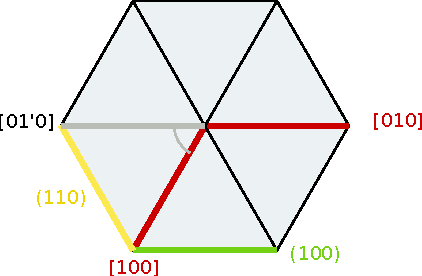
\includegraphics[]{figures/2_4Hexa.pdf}
            \caption{\{100\} enthält (100), aber nicht (1$\overline{1}$0)\\
            $\rightsquigarrow$ 4. Index $i = -(h+k)$: hkil also für obiges Beispiel {10$\overline{1}$0}}
            \label{}
        \end{figure}
	\end{itemize}
\end{itemize}
\section{Strukturanalyse} \label{kap:3}
\begin{itemize}
    \item[(a)] Direkte Abbildung:\\
          \begin{itemize}
              \item Transmissions-Elektronen-Mikroskopie (TEM)
              \item Raster-Tunnel-Mikroskopie (STM)
          \end{itemize}
          Atomare Auflösung, aber nur oberflächenintensiv
    \item[(b)] \textbf{Beugungs-/ Streuexperimente:}\\
          Grundidee:
          \begin{itemize}
              \item Einstrahlung einer Welle (elektromagnetische Welle, Materiewelle) auf den periodischen Festkörper (Gitterkonstante $a \approx$ 1 \AA)\\
                    Bedingung für Beugung: $\lambda < \approx a$\\
                    z.B. Röntgenstrahlung mit $\lambda \approx$ 1 \AA ($h \nu$ = 12 keV)\\
                    Elektronen mit $\lambda \approx$ 1 \AA ($h \nu$ = 150 eV)\\
                    Neutronen mit $\lambda \approx$ 1 \AA ($h \nu$ = 80 meV)\\
                    He-Atome mit $\lambda \approx$ 1 \AA ($h \nu$ = 20 meV)
              \item Je nach Art der Welle unterschiedliche Eindringtiefe Röntegen- u. Neutronensteuung $\rightarrow$ massive FK, Elektronen - u. Atomstreuung eher für dünne Filme / Oberflächen.
              \item Je nach Art der Welle Information über Elektronen- bzw. Kernverteilung. Beugungsmuster bei bekannten $\lambda$ liefert Informationen über periodische Anordnung des Kristalls.\\
                    Man unterscheidet
                    \begin{itemize}
                        \item \textbf{Kohärente Streuung} (Information über Struktur) oder inkohärente Streuung
                        \item \textbf{Elastische Streuung} (Strukturbestimmung) oder inelastische Streuung (Untersuchung von elektronischen oder vibronischen Anregungen)
                    \end{itemize}
          \end{itemize}
\end{itemize}





\subsection{Einführung in die Streutheorie} \label{kap:3_1}
Grundannahmen: Klassische Beschreibung der Streuung, elastische Streuung, Einfachstreuung
\begin{itemize}
    \item Einlaufende Welle und auslaufende Welle sind eben Wellen (Guta Annahme, falls Quelle bzw. Beobachter weit entfernt)
          \begin{figure}[H]
              \centering
              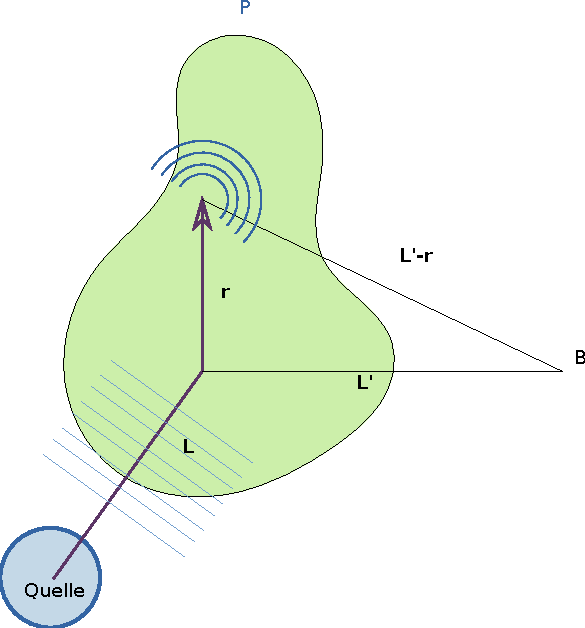
\includegraphics{figures/2_4Birne.pdf}
              \caption{}
              \label{}
          \end{figure}
    \item Einlaufende welle mit Amplitude $A_P = A_0 e^{-i(\omega_0 t - \textbf{k} ( \textbf{L} + \textbf{r}))}$
    \item Auftreffen auf Verteilung von Streuzentren mit komplexwertiger Streudichteverteilung $\rho(\textbf{r})$, die vom Ort und von Art der WW abhängt.
    \item Jedes Streuzentrum (z.B. P) emittiert eine Kugelwelle, deren Amplitude und Phase relativ zur einlaufenden Welle con $\rho(\textbf{L} + \textbf{r})$ abhängt.
          \begin{align*}
              A_B^P                   & = A_P \cdot \rho(\textbf{L} + \textbf{r}) \frac{e^{i\textbf{k}' ( \textbf{L}' - \textbf{r})}}{|\textbf{L}' - \textbf{r}|}                                                                   \\
                                      & \approx \frac{A_0}{L'} e^{-i \omega_0 t} e^{i \textbf{k} \textbf{L}} e^{i \textbf{k}' \textbf{L}'} \rho(\textbf{L} + \textbf{r})  e^{i \textbf{k} \textbf{r}} e^{i \textbf{k}' \textbf{r}'}
              A_B (\Delta \textbf{k}) & = \tilde{A} \int \delta(\textbf{r})e^{-i \Delta\textbf{kr}}d^3r
          \end{align*}
          Streuexperimente messen die Intensität, nicht die Amplitude
          \begin{align*}
              I(\Delta \textbf{k}) \sim \left| A_B(\Delta \textbf{k}) \right|^2
          \end{align*}
          $\rightarrow$ Streudichteverteilung kann nicht direckt durch Rücktransformation
          \begin{align*}
              \delta(\textbf{r}) = \frac{1}{(2\pi)^3}\int A_B(\Delta \textbf{k}) e^{i \Delta\textbf{kr}} dk
          \end{align*}
          bestimmt werden, da nur $\left|A_B(\Delta \textbf{k}) \right|$ bekannt ist (Phasenproblem)
\end{itemize}




\subsection{Das reziproke Gitter} \label{kap:3_2}
Kristallstrukturen sind trasnlationsinvariant, somit ist
\begin{align*}
    \rho(\textbf{r}) = \delta(\textbf{r}+\textbf{R})
\end{align*}
mit Gittervektor $\Leftrightarrow \textbf{R} = n_1 \textbf{a}_1 + n_2 \textbf{a}_2 + n_3 \textbf{a}_3$.\\
Damit Entwicklung im Fourrier-Reihe
\begin{align*}
    \rho(\textbf{r}) = \sum_{h,k,l}\rho_{hkl} e^{i \textbf{G}_{hkl}\cdot r}
\end{align*}
mit
\begin{align*}
    \rho_{hkl} = \frac{1}{V_0}\int_{V_0}e^{i \textbf{G}_{hkl}\cdot r}d^3r
\end{align*}

$V_0$ Intergration über 1 Periode, d.h. primitive EZ.
\begin{itemize}
    \item[(a)] \textbf{Reziprokes Gitter}\\
          Der Vektor $\textbf{G}_{hkl}$ kann durch Basisvektoren $\textbf{b}_1, \textbf{b}_2, \textbf{b}_3$ dargestellt werden
          \begin{align*}
              \textbf{G}_{hkl} = h \textbf{b}_1 + k \textbf{b}_2 + l \textbf{b}_3
          \end{align*}
          \begin{itemize}
              \item $\textbf{G}_{hkl}$ sind Gittervektoren eines neuen Gitters, des \textbf{reziproken Gitters}
              \item Translationsinvarianz im \textbf{realen Gitter (Ortsgiller)}:
                    \begin{align*}
                        \rho(\textbf{r})  \overset{!}{=}  \rho(\textbf{r} + \textbf{R}) = \sum_{h,k,l} \rho_{hkl} e^{i \textbf{G}_{hkl} (\textbf{r}+\textbf{R})} \quad \Rightarrow \quad e^{i \textbf{G}_{hkl} \textbf{R}} \overset{!}{=} 1 \\
                        \Leftrightarrow \quad \textbf{G}_{hkl} \textbf{R} = 2 \pi m \quad (m \in \mathbb{Z})
                    \end{align*}
                    Für belibige Koeffizienten $ \textbf{n}_1, \textbf{n}_2, \textbf{n}_3$ von $\textbf{R}$ und $h,k,l$ von $G_{hkl}$ dies nur  falls $\textbf{a}_i\cdot \textbf{b}_j > 2\pi \delta_{ij} (i,j = 1,2,3)$
                \item[$\rightsquigarrow$] Damit lauten die Basisvektoren des reziproken Gitters:
                \begin{align*}
                    \textbf{b}_1 &= \frac{2 \pi}{V_0} ( \textbf{a}_2 \times \textbf{a}_3)\\
                    \textbf{b}_2 &= \frac{2 \pi}{V_0} ( \textbf{a}_3 \times \textbf{a}_1)\\
                    \textbf{b}_3 &= \frac{2 \pi}{V_0} ( \textbf{a}_1 \times \textbf{a}_2)
                \end{align*}
                und das Volumen der primitiven EZ des reziproken Gitters:
                \begin{align*}
                    \textbf{b}_1 ( \textbf{b}_2 \times \textbf{b}_3) &= \frac{(2 \pi)^3}{V_0} \quad \text{mit} \quad V_0 = \textbf{a}_1 ( \textbf{a}_2 \times \textbf{a}_3)
                \end{align*}
          \end{itemize}
          \textbf{Bemerkung:}
          \begin{itemize}
              \item Jedem rez. GV $\textbf{G}_{hkl}$ ist ein Fourier-Koeffizient $\rho_{hkl}$ eindeutig zugeordnet
              \item Reziproke Gittervektoren haben Dimension 1/Länge, daher Bezeichnung \textit{reziprokes Gitter}.
              \item Reziproke Gittervektoren existieren nicht im Ortsraum, sondern im reziproken Raum. (Fourierraum,b-Raum, Impulsraum wegen $\textbf{p}= \hbar \textbf{k}$)
          \end{itemize}
          \begin{table}[htbp]
              \centering
              \caption{Beispiele}
              \begin{tabular}{ccc}
                  \hline
                  Beispiele & Real                & Reziprokes                                                            \\ \hline
                  1D        & o-o-o (distanz = a) & o-o-o  (distanz $= b \frac{2\pi}{a}$)                                 \\
                  2D        & vgl Folie \#4       & $\textbf{b}_1 \bot \textbf{a}_2$ und $\textbf{b}_2 \bot \textbf{a}_1$ \\
                  3D        & SC mit a            & SC mit $b=\frac{2\pi}{a}$                                             \\
                            & bcc                 & fcc                                                                   \\
                            & fcc                 & bcc                                                                   \\ \hline
              \end{tabular}
          \end{table}

          \begin{itemize}
              \item[sc:]
                    \begin{align*}
                        \textbf{a}_1 & = a \left(\begin{array}{c} 1 \\ 0 \\ 0 \end{array}\right) , \textbf{a}_2 = a \left(\begin{array}{c} 0 \\ 1 \\ 0 \end{array}\right) , \textbf{a}_3 = a \left(\begin{array}{c} 0 \\ 0 \\ 1 \end{array}\right) , V_0 = \dots = a^3 \\
                        \textbf{b}_1 & = \frac{2 \pi}{a^3} (\textbf{a}_2 \times \textbf{a}_3) = \frac{2 \pi }{a} \left(\begin{array}{c} 1 \\ 0 \\ 0 \end{array}\right)                                                                     \\
                        \textbf{b}_2 & = \frac{2 \pi}{a^3} (\textbf{a}_3 \times \textbf{a}_1) = \frac{2 \pi }{a} \left(\begin{array}{c} 0 \\ 1 \\ 0 \end{array}\right)                                                                     \\
                        \textbf{b}_3 & = \frac{2 \pi}{a^3} (\textbf{a}_1 \times \textbf{a}_2) = \frac{2 \pi }{a} \left(\begin{array}{c} 0 \\ 0 \\ 1 \end{array}\right), V_R = (\frac{2 \pi}{a})^3
                    \end{align*}
              \item[bcc:]
                    \begin{align*}
                        \textbf{a}_1 = \frac{a}{\sqrt{2}} \left(\begin{array}{c} -1 \\ 1 \\ 1 \end{array}\right), \textbf{a}_2 = \frac{a}{\sqrt{2}} \left(\begin{array}{c} 1 \\ -1 \\ 1 \end{array}\right), \textbf{a}_3 = \frac{a}{\sqrt{2}} \left(\begin{array}{c} 1 \\ 1 \\ -1 \end{array}\right)
                    \end{align*}
                    GV des bcc-zugehörigen primitiven Gitters
              \item[fcc:]
                    \begin{align*}
                        \textbf{a}_1 = \frac{a}{2} \left(\begin{array}{c} 0 \\ 1 \\ 1 \end{array}\right), \textbf{a}_2 = \frac{a}{2} \left(\begin{array}{c} 1 \\ 0 \\ 1 \end{array}\right), \textbf{a}_3 = \frac{a}{2} \left(\begin{array}{c} 1 \\ 1 \\ 0 \end{array}\right)
                    \end{align*}
          \end{itemize}

    \item[(b)] \textbf{Brillouin-Zonen}\\
          Analog zu den Gitter lässt sich auch in res. Gitter die   Wigno-Seitz-Zelle konstruieren. Sie wird als 1. Bernoulli Zelle bezeichnet, und ist entscheidend für Eigenschaften von Festkörpern.\\
          Durch Erweiterung des Konstruktionsprinzips auf weiter entfernte rez. Gitterpunkte lassen sich \textbf{BZ höherer Ordnungen} definieren.
          \begin{center}
              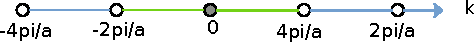
\includegraphics{figures/3_2_1D.pdf}
          \end{center}
          \begin{figure}[H]
              \centering
              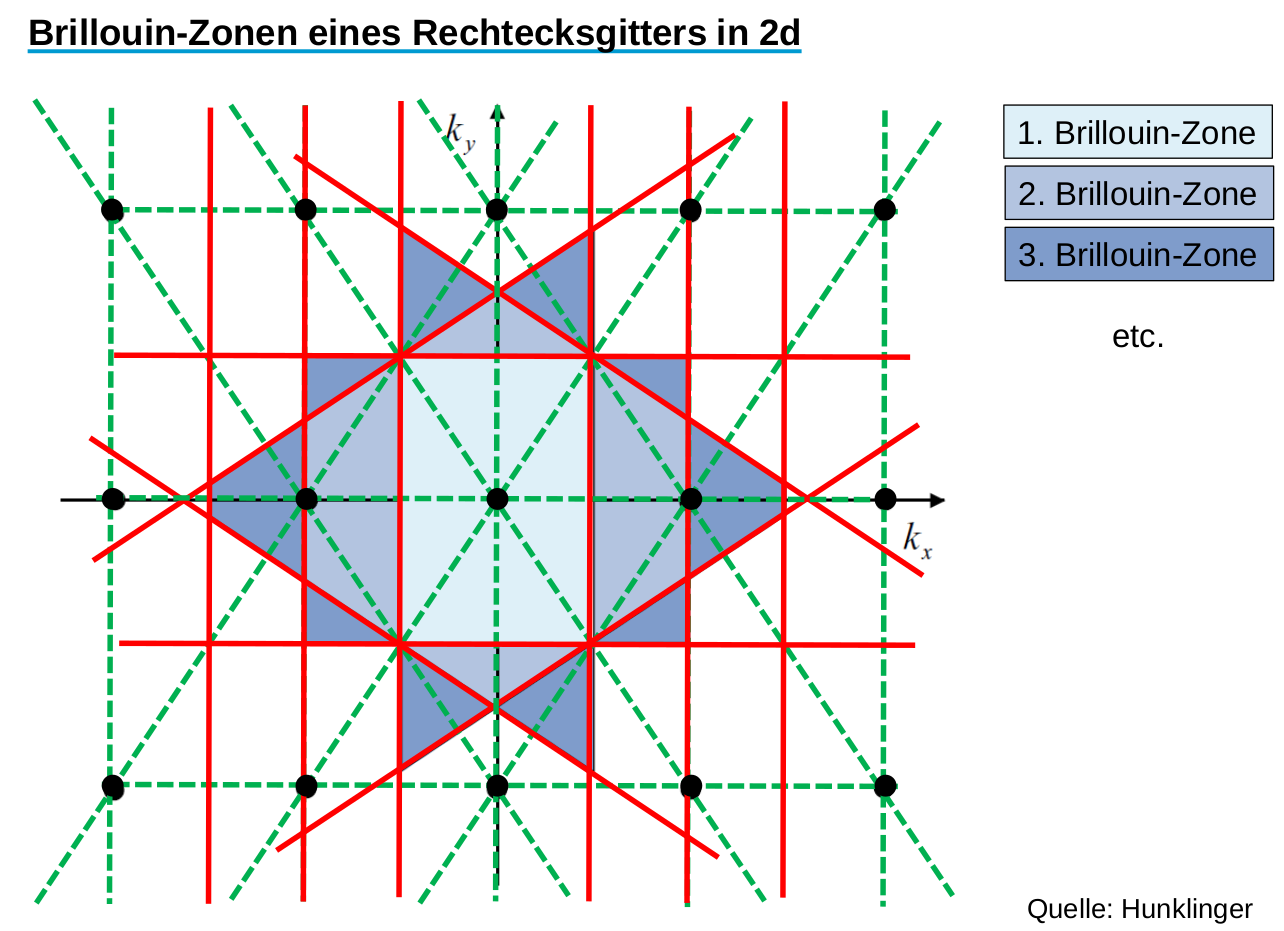
\includegraphics[width=0.6\textwidth]{figures/3_2_2D.png}
              \caption{Brillouin-Zonen 2D}
              \label{}
          \end{figure}
          Rechtecksgitter:
          \begin{itemize}
              \item[1. BZ:] Rechteck
              \item[2. BZ:] 4 Teilflächen, die sich durch Verschiebung um \textbf{rez. Gitterverktoren} zu Rechteck der 1. BZ Zusammensetzen lassen.
              \item[3. BZ:] (und höhere) Je höher die Ordnung der BZ, desto mehr/komplizierte Teilflächen. Durch Verschiebungum rez. GV $\Rightarrow$ Rückführung auf 1. BZ
          \end{itemize}
          \begin{figure}[H]
              \centering
              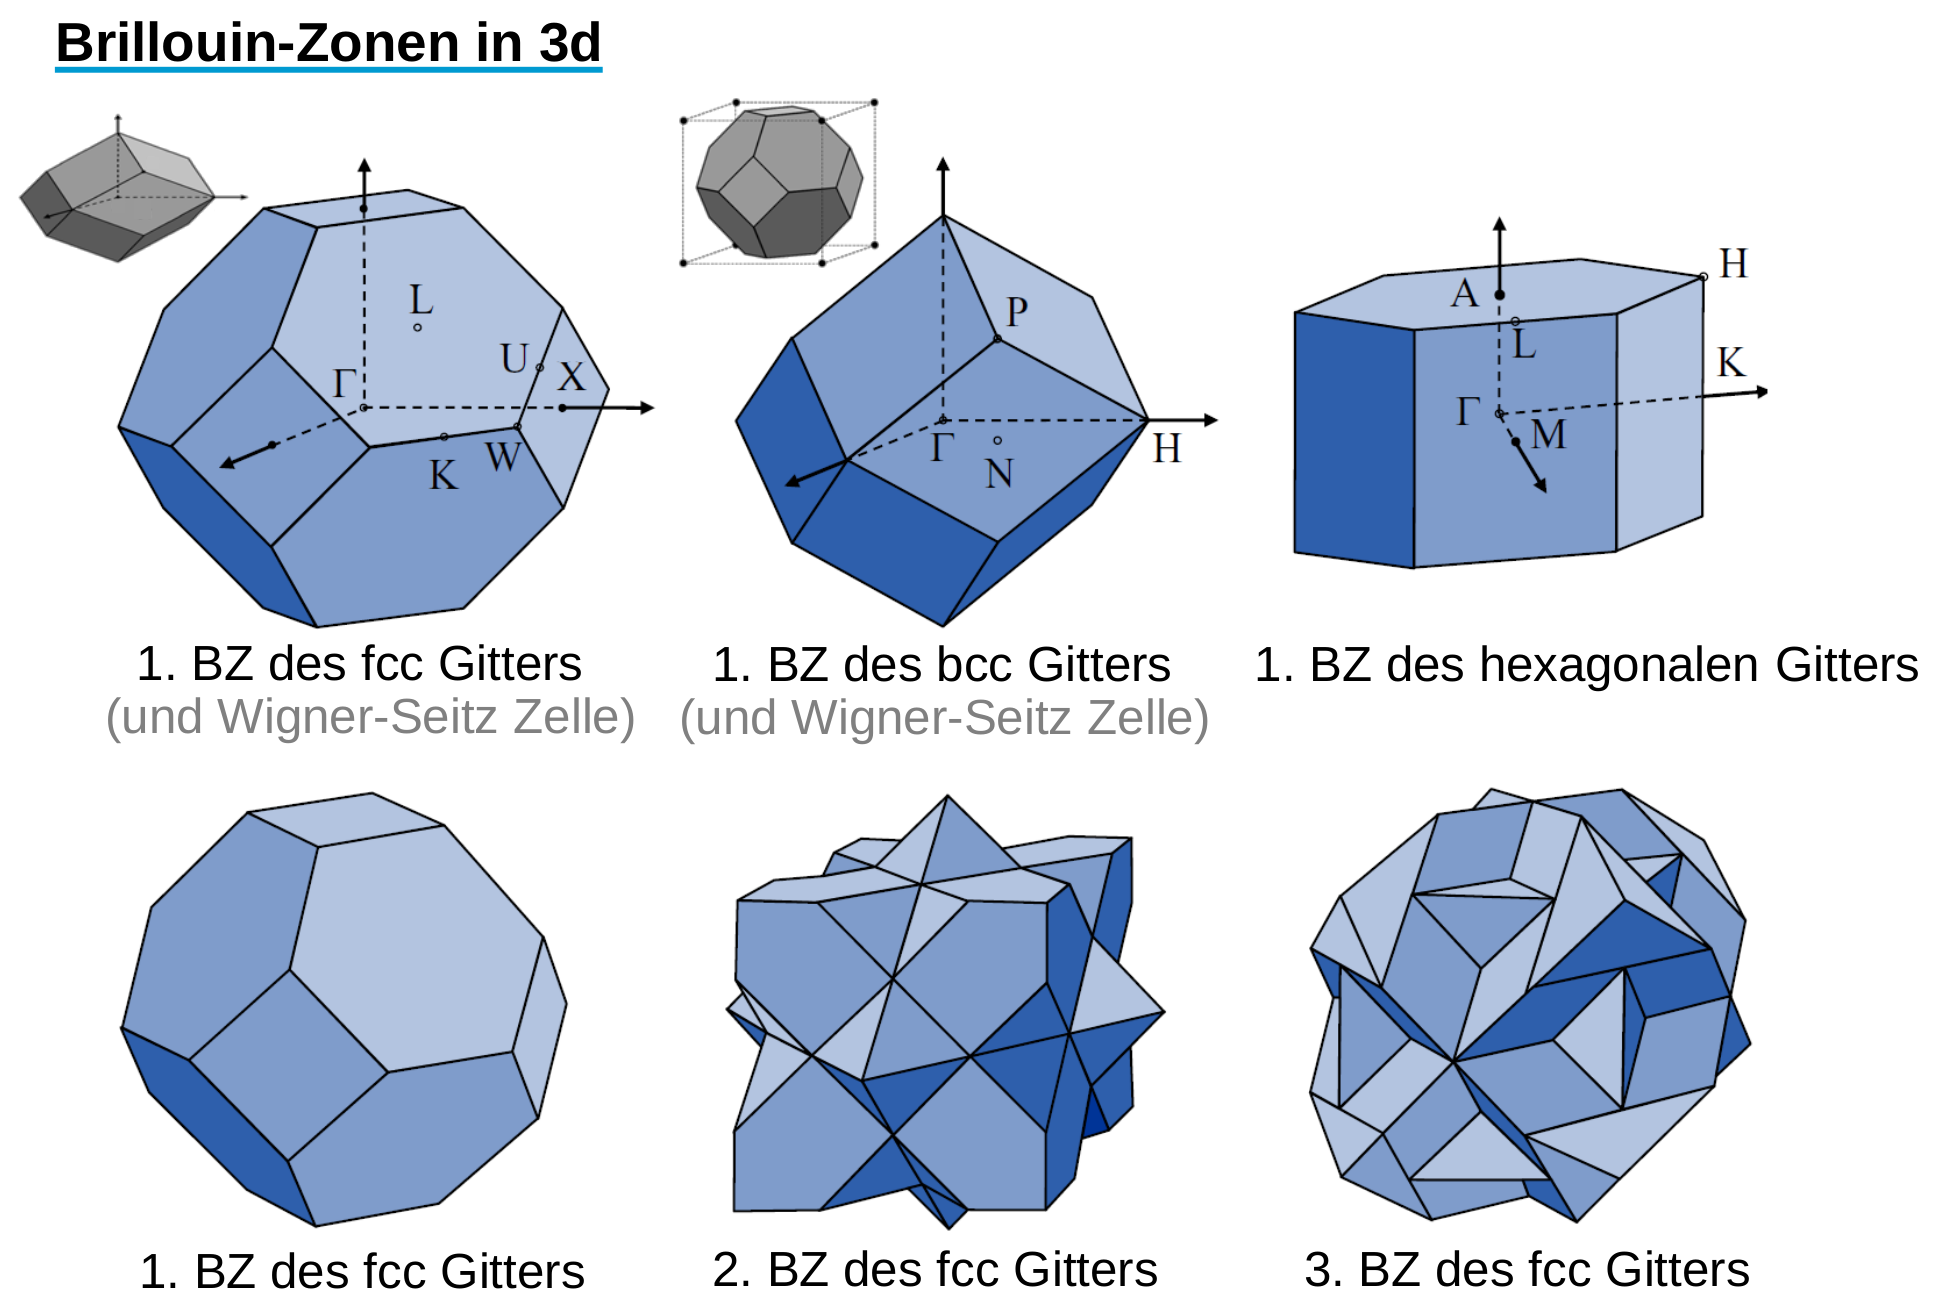
\includegraphics[width=0.6\textwidth]{figures/3_2_3D.png}
              \caption{Brillouin-Zonen 3D}
              \label{}
          \end{figure}
          Auch in 3D: BZ höherer Ordnung aus immer mehr Einzelteilen zusammengesetzt. Durch Verschiebung um rez. GV erhält man Polyeder, der in Größe und Gestalt der 1. BZ entspricht.\\
          \textbf{Diskussion:}
          \begin{itemize}
              \item 1. BZ ist Wigner-Seitz-Zelle des rez. Raums
              \item Durch periodischs Aneinanderreihen der 1. BZ lässt sich der reziproke Raum vollständig auffüllen.
              \item Punkt hoher Symmetrie werden Symbole ($\rightsquigarrow$ Gruppentheorie) zugeordnet, z.B. $\Gamma$-Punkt: Zentrum der 1. BZ, X-Punkt: Schnittpunkt der 1. BZ mit x.Achse
          \end{itemize}
    \item[(c)] \textbf{Miller-Indizes}
          Zwischen den Miller-Indizes zur Bezeichnung von Gitterelementen des realen Gitters und dem reziproken Gitter besteht ein direkter Zusammenhang:\\
          \begin{itemize}
              \item[1.] Der reziproke Gittervektor $\textbf{G}_{hkl}$ steht senkrecht auf den Netzebenen (hkl) im realen Raum.\\
                    Begründung:
                    \begin{align*}
                        \textbf{G}_{hkl} & = h \textbf{b}_1 + k \textbf{b}_2 + l \textbf{b}_3\\
                        & =\frac{2 \pi}{V_0}\left[h(\textbf{a}_2\times \textbf{a}_3) + k(\textbf{a}_3\times \textbf{a}_1) + l(\textbf{a}_1\times \textbf{a}_2)\right]
                    \end{align*}
                    vgl. Normalvektor auf $(hkl)$ \textbf{n}\\
                    $e^{i \textbf{G}_{nlk}\textbf{R}}$ und also hier $\textbf{n} e^{i \textbf{n} \textbf{R}} \overset{!}{=}1$ folgt $\textbf{n} \parallel \textbf{G}_{hkl}$.
              \item[2.] Der Abstand zweier benachbarter Netzebenen im realen Raum ist durch den Betrag des kürzesten reziproken Gittervektors $\left| \textbf{G}_{nlk}^{min} \right|$ bestimmt:
              $$d_{hkl} = \frac{2 \pi}{\left| \textbf{G}_{nlk}^{min} \right|} $$
              Begründung: Für $\left| \textbf{G}_{nlk}^{min} \right| = \frac{2 \pi}{d_{hkl}}$ ist $e^{i \textbf{G}_{nlk}^{min} \textbf{R}} = 1$ mit $\lambda = 2 \pi \left| \textbf{G}_{nlk}^{min} \right|^{-1} = d_{hkl}$
          \end{itemize}
\end{itemize}



\subsection{Streuung an Kristallen} \label{kap:3_3}
Streuintensität:
\begin{align*}
    I(\Delta \textbf{k}) \sim |A_B (\Delta \textbf{k})|^2 \sim \left| \int_{V} \rho(\textbf{r})e^{-i \Delta \textbf{k} \cdot \textbf{r}} \mathrm{d}^3r\right|^2 = \left|\mathcal{A}(\Delta\textbf{k})\right|^2 
\end{align*}
mit Streuvektron $\Delta \textbf{k} = \textbf{k}_2-\textbf{k}_1$
\begin{itemize}
    \item Vorfaktoren sind zunächst nicht von Bedeutung, da Abhängigkeit von $I$ con$\Delta \textbf{k}$ untersucht
    \item Vorsicht: In der Literatur werden manchmal $A_B$ und $\mathcal{A}$ als Streuamplitude bezeichnet.
\end{itemize}
Mit Kap. \ref{kap:3_2}:
\begin{align*}
    \left| \mathcal{A} ( \Delta \textbf{k}) \right| ^2 = \left| \sum_{hkl} \rho_{hkl} \int_V e^{i(\textbf{G} - \Delta \textbf{k})\textbf{r}} \mathrm{d}^3 r \right|^2
\end{align*}

\begin{itemize}
    \item[$\rightarrow$] Im allgemeinen Fall $\Delta \textbf{k} \neq \textbf{G}$:$e$-Funktion hat kompexe Exponenten und oszilliert. Bei großem V (d.h. größer als Oszillationsperiode $\left(1 /(\textbf{k}\cdot \textbf{G})\right)^3$) mitteln sich die Beträge weg.\\
    Physikalisch: Streubeiträge der einzelnen Atome interferieren destruktiv.
    \item[$\rightarrow$] Spezialfall $\Delta \textbf{k} = \textbf{G}$: e-Funktion hat den Wert 1.\\
    Physikalisch: Beiträge der einzelnen interferieren konstruktiv.
\end{itemize}

\begin{align*}
    \left| \mathcal{A} ( \Delta \textbf{k}) \right| ^2 = \begin{cases}
        0 & \text{für } \Delta \textbf{k} \neq \textbf{G}\\
        \left| \rho_hkl\right|^2 \cdot V^2 &  \text{für } \Delta \textbf{k} = \textbf{G}_{(hkl)}
    \end{cases}
\end{align*}
\begin{itemize}
    \item Streuung am Kristall: Streusignal $\neq 0$ nur, wenn Bedingung $\Delta \textbf{k} = \textbf{G}$ erfüllt. (Von Laue Bedingung)
    \item Bei realen Kristallen endliches V, endliche Eindringtiefe der Bedingung\dots
    \item Bei fester Lage der Probe (Kristalls) tritt in den meisten Richtungen keine Streuung auf. Bei Beugungsexperimente muß Kristallorientirung so lange gedreht werden, bis $\Delta \textbf{k} = \textbf{G}$, also ein Streusignal (Beugungsreflex) auftritt.
    \item Warum $\sim V^2$?\\
    $|\mathcal{A}(\Delta \textbf{k})|^2$ entspricht Intensität im Maximum des Beugungsreflexes Endliches V führt zu Verbreiterung $\sim V$\\
    Intergrierte Intensität des Beugungsreflexes $\sim \frac{V^2}{V} = V \sim$ Anzahl der Streuzentren.\\
    Auch Eindringtiefe trägt zu Verbreiterung bei. Z.B. Röntgenstrahlung: $10^{-5}-10^{-3}$ pro Netzebene.
\end{itemize}

\begin{itemize}
    \item[(a)] Ewald-Kugel und Bragg Bedingung\\
    \textbf{Ewald Konstruktion:}
    \begin{itemize}
        \item[(1)] Zeichne reziproke Gitter, wähle Gitterpunkt
        \item[(2)] Einzeichnen von einfallendem Wellenvektor als \textbf{-k} von diesem
        \item[(3)] Endpunkt von $-\vk$ (Anfang von \textbf{k}) sei Mittelpunkt der \textbf{Ewald-Kugel} (2D: Ewald-Kreis) mit Radius k.
        \item[(4)] Für rez. Gitterpunkte, die auf dieser Kugel liegen, ist von Laue Bedinugn $\dvk = \vk' - \vk \overset{!}{=} \textbf{G}$ erfüllt. Der gebeugte Strahl tritt dann mit Wellenvektro $\vk' = \vk + \textbf{G}$ aus. In dieser Richtung tritt Beugungsreflex auf.
        \item[(5)] Verschmierung der reziproken Gitterpunkte $\rightarrow$ endliches Probenvolumen.
    \end{itemize}
    \textbf{Diskussion:}\\
    Durch expt. Anordnung des Beugungsexperiments und ORientierung der Probe liegt $\dvk$ bzgl. des reziproke Gitters fest.\\
    $\rightarrow$ Beugungsreflex $\rightarrow \textbf{G}_{hkl} \rightarrow \rho_{hkl} \rightarrow \textbf{G}_{hkl} \bot (hkl)$\\
    d.h. Beugungsreflex resultiert aud Streuung an Netzebenenschar, also periodischen Streudichtevariation mit Periode $d_{hkl}$. Zusammenhang von Laue Bedingung und Bragg-Bedingugn Betrachte Steuung als Funktion des Winkel $\Theta$ zwsche $\vk$ und (hkl).
    \begin{figure}[H]
        \centering
        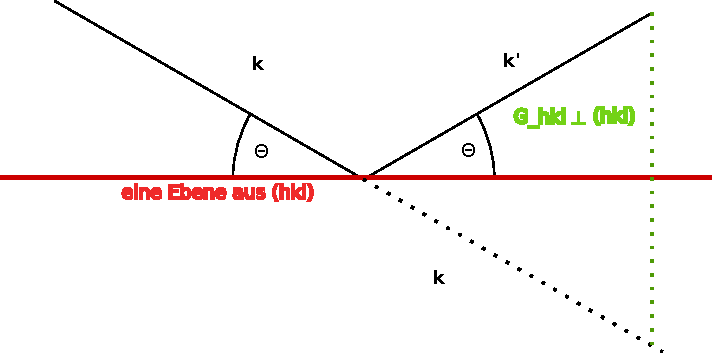
\includegraphics{figures/3_3Reflection.pdf}
        \caption{$|\textbf{G}_{hkl}|=2\cdot k \sin(\Theta) = \frac{4\pi}{\lambda}\sin(\Theta)$ mit $\lambda=\frac{2\pi}{k}$\\ }
        \label{fig:3_3Reflection}
    \end{figure}
    mit (2) 
    \begin{align*}
        \textbf{G}_{hkl} = n \textbf{G}_{hkl}^{min} n\frac{2\pi}{\textnormal{d}_{hkl}} = \frac{4\pi}{\lambda}\sin{\Theta} \Longleftrightarrow 2\cdot \textnormal{d}_{hkl}\sin{\Theta}= n \lambda
    \end{align*}
    \item[(b)] Strukturfaktor:\\
    Bisher nur Ort von Beugungsreflexen ($\Delta \textbf{k} = \textbf{G})$, für Intensitäten wird Fourier-Koeffizient
    \begin{align*}
        \rho_{hkl} = \frac{1}{V_0} \int_{V_0} \rho (\textbf{r}) e^{-i \textbf{G} \textbf{r}} \mathrm{d}^3r \quad \text{mit } V_0 \text{ primitive EZ}
    \end{align*}
    \begin{itemize}
        \item[$\rightarrow$] Information über Aufbau der Basis.\\
        Streubeiträge der Basisatome können konstruktiv o. destruktiv interferieren.
        \begin{itemize}
            \item[$\rightarrow$] Stärke des Beugungsreflexes
        \end{itemize}
    \end{itemize}
    Aufteilung der Streudichteverteilung af Basisatome:
    \begin{align*}
        \textbf{r} = \textbf{R}_n + \textbf{r}_\alpha + \textbf{r}'
    \end{align*}
    $\textbf{R}_n$: Ursprung EZ, $\textbf{r}_\alpha$: $\alpha$-tes Atom, $\textbf{r}'$: Ortsvektor von $\alpha$-tem Atom.\\
    mit:
    \begin{align*}
        \textbf{r}_\alpha = u_\alpha \textbf{a}_1 + v_\alpha \textbf{a}_2 + w_\alpha \textbf{a}_3
    \end{align*}
    \begin{itemize}
        \item[$\rightsquigarrow$] Für jede Art von streuender Welle und zugehöriger WW gerechtfertigt, weil die Streudichteverteilung immer noch um Atom konzentriert ist.
    \end{itemize}
    \begin{itemize}
        \item Röntgenbeugung: Schalenelektronen
        \item Neutronenbeugung: Kernen
    \end{itemize}
    \begin{align*}
        \Rightarrow \qquad \rho_{hkl} = \frac{1}{V_0} \sum_{\alpha} e^{-i \textbf{G} \textbf{r}_{\alpha}} \underbrace{\int_{V_{\alpha}} \rho_{\alpha} (\textbf{r}') e^{-i \textbf{G} \textbf{r}'} \mathrm{d}^3r'}_{=: f_{\alpha} (\textbf{G})\text{ Atom-Formfaktor ($\rightarrow c$)}}  = \frac{1}{V_0} \underbrace{\sum_{\alpha} e^{-i \textbf{G} \textbf{r}_{\alpha}} f_{\alpha} (\textbf{G})}_{=: S_{hkl}}
    \end{align*}
    $\text{Strukturfaktor:} \qquad S_{hkl} = \sum_{\alpha} e^{-i \textbf{G} \textbf{r}_{\alpha}} f_{\alpha} (\textbf{G})$
        \begin{itemize}
        \item[$\rightarrow$] Beschreibt Einfluss der Interferenz der Basisatome auf dei Streuverteilung.
        \begin{align*}
            S_{hkl} = \sum_\alpha f_\alpha e^{-2\pi i (hu_\alpha+kv_\alpha+lw_\alpha)}
        \end{align*}
        \item[$\rightarrow$] \textbf{Spezialälle:}
        \begin{itemize}
            \item[(i)] Primitives Gitter (nur 1 Atom im Ursprung) $S_{hkl}=f(\textbf{G})$
            \item[(ii)] CsCl Gitter\\ $\text{Kubisch primitiv mit 2-atomiger Basis} \qquad \textbf{r}_{Cs}= \left(\begin{array}{c} 0 \\ 0 \\ 0 \end{array}\right) \textbf{r}_{Cl} = \left(\begin{array}{c} 1/2 \\ 1/2 \\ 1/2 \end{array}\right)$ 
            \begin{align*}
                S_{hkl} = \begin{cases}
                    f_{Cs} & \text{für $h+k+l$ gerade}\\
                    f_{Cl} & \text{für $h+k+l$ ungerade}
                \end{cases}
            \end{align*}

            \item[(iii)] bcc Giter (einfache Basis): \textbf{r}$_1 = \left(\begin{array}{c} 0 \\ 0 \\ 0 \end{array}\right)$, \textbf{r}$_2 = \left(\begin{array}{c} 1/2 \\ 1/2 \\ 1/2 \end{array}\right)$
            \begin{align*}
                S_{hkl} = \begin{cases}
                    2f & \text{für $h+k+l$ gerade}\\
                    0 & \text{für $h+k+l$ ungerade}
                \end{cases}
            \end{align*}

            \item[\textbf{Diskussion}]
            Im bcc Gitter (und in anderen zentrierten Gittern) Kommte es zur systematischen Anslöschung von Beugungsreflexen.\\
            Ursache: Destruktive Interferenz der Netzebene durch das im Ursprung liegende Atom und das Zentrierte Atom.
            \item[\textbf{Beispiel}(100)] (Beugungsreflex)
                \begin{figure}[H]
                    \centering
                    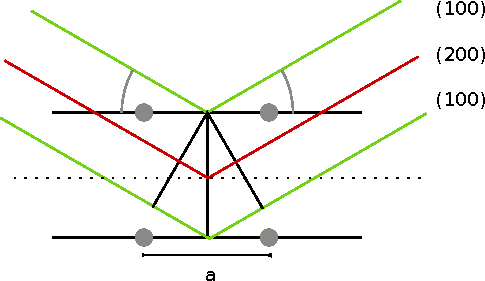
\includegraphics[]{figures/3_3Bragg.pdf}
                    \caption{}
                    \label{}
                \end{figure}
              % TODO
        \end{itemize}
    \end{itemize}
    \item[(c)] \textbf{Atomformfaktor}\\
    Streuvermögen eines einzelnen Atoms $f_\alpha(\Delta \textbf{k}) = \int_{V_\alpha}\rho_\alpha(r_\alpha)e^{-i\Delta \textbf{k} \textbf{r}'} d^3r'$ \\
    {\footnotesize mit $\Delta \textbf{k} = \textbf{G}$}\\
    $\rightarrow$ Art der Wechselwirkung zwischen Welle und Atom.
    \begin{itemize}
        \item[(i)] \textbf{Neutronenstreuung}\\
        Streuung am Kern, Punktförmig, $\Delta \textbf{k} \cdot \textbf{r} \ll 1$
        \begin{align*}
            f_{\alpha} (\Delta \textbf{k}) = \int_{v_{\alpha}} \rho_{\alpha} (\textbf{r}') \mathrm{d}^3r' = -b
        \end{align*}
        -: Konvention, gemessen wird $|b|^2$\\
        $b$: Streulänge
        \item[(ii)] \textbf{Röngensteruung}
        Streuung an Elektronenhühlle $\sim a \sim \lambda$
        Annahme: kugelsymmetrische Ladungsdichteverteilung:
        \begin{align}
            f_\alpha(\Delta \textbf{k}) &= 
            \int_{0}^{R_\alpha} \mathrm{d}r
            \int_{0}^{\pi} \mathrm{d}\theta
            \int_{0}^{2\pi} \mathrm{d}\phi \rho_\alpha(r) r^2 \sin(rl)e^{-i\Delta k r \cos{\theta}}\nonumber\\
            &= \int_{0}^{R_\alpha}4\pi r^2 \rho(r)\frac{\sin{\Delta k \cdot r}}{\Delta k \cdot r} \mathrm{d}r \label{eq:rstr}
        \end{align} 
        z.B. H-Atom:
        \begin{align*}
            \rho (r) = \left| \Psi_0 (r) \right|^2 = \left| \sqrt{\frac{1}{\pi a_0^3}} \cdot e^{-r/a_0} \right| ^2 = \frac{1}{\pi a_0^3} \cdot e^{-2r/a_0}
        \end{align*}
        in (\ref{eq:rstr}) und Limes $R_{\alpha} \rightarrow \infty$:
        \begin{align*}
            f_H (\Delta k) = \left[ \frac{1}{1+(\frac{1}{2} a_0 \Delta k)^2}\right]^2
        \end{align*}
        Vereinfachung für $\Delta k \cdot r \rightarrow 0$:
        \begin{align*}
            \lim_{\Delta k r \rightarrow 0}f_H(\Delta k) = \int_0^{R_\alpha}4\pi r^2 \rho(r)\dr = Z\\
            \rightarrow \qquad f_H = Z \quad \text{oder Streuintensität} \quad \sim Z^2
        \end{align*}
        Erfüllt für:\begin{itemize}
            \item Vorwärtsstreuung ($\Delta k = 0$)
            \item Näherungsweise punktförmige Atome ($R_\alpha \ll  a \approx \lambda$)
        \end{itemize}
    \end{itemize}
    \item[(d)] \textbf{Debye-Waller-Faktor}
    Berücksichtigt die thermische Fluktuation der Atome um ihre Gleichgewichtsposition.
\end{itemize}



\subsection{Experimentelle Methoden der Strukturanalyse durch Beugung} \label{kap:4_4}
\begin{itemize}
    \item[(a)] \textbf{Messverfahren}
    \begin{itemize}
        \item[(i)] \underline{Drehkristallverfahren:}\\
        Voraussetzung - Einkristall; - monochromatische Strahlung (festes $\lambda$)\\
        Messprinzip: Voraussetzung $\Delta \textbf{k} = \textbf{G}$ ist bei gegebenem $\Delta \textbf{k}$ in der Regel nicht erfüllt. Drehung des Kristalls um eine Achse. Für bestimmte Winkel ist Streubedingung für bestimmte Netzebenenschar erfüllt.\\
        Nach Möglichkeit Drehachse = Symmetische Achse de Kristalls, z.B. $\textbf{a}_3$
        \begin{itemize}
            \item[$\rightarrow$] Netzebenen $||$ Drehachse: \textbf{G}$_{nk0}$ (l=0)\\
            Streuung in xy Ebene, Reflexe falls $\Delta k$ = $G_{hk0}$
            \item[$\rightarrow$] Netzebenen $\nparallel$ Drehachse: $\textbf{G}_{hkl}$\\
            Streuung ausserhalb xy-Ebene, vertikale Verschiebung der Beugungsreflexe für $l = \pm 1, \pm 2, \dots$
            % \begin{figure}[H]
            %     \centering
            %     \includegraphics[]{}
            %     \caption{Typische Detektion mit zylindrischem Film.}
            % \end{figure}
	   \end{itemize}
	   \item[ii)] Debye-Scherrer-Verfahren (Pulvermethode):
		Kristallpulver (Kristallite mit zufällig orientierter Richtung), monochromatische Strahlung.\\
		\textbf{Messprinzip:}  Streubedingung $\Delta \textbf{k} = \textbf{G}$ lässt sich für festes \textbf{k} immer erfüllen (durch passend orientierte Kristallite)\\
		$\rightarrow$ Alle Beugungsreflexe zu festem \textbf{G} liegen auf einem Kegelmantel der konzentrisch zum einfallenden Strahl ausgerichtet ist und Öffnungswinkel $2\Theta$ besitzt.
		\begin{figure}[H]
			\centering
			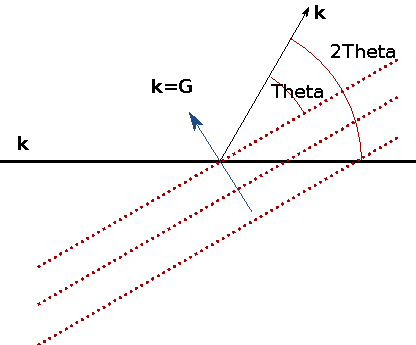
\includegraphics{figures/3_4RefKrist.pdf}
			\caption{Vorteile, sehr präzise, z.B. Bestimmung von Gitterkonstanten}
			\label{}
		\end{figure}
		\item[iii)] Laue-Verfahren:
		Einkristall, Kontinuumsstrahlung ('alle' $\lambda$) Messprinzip: $\Delta \textbf{k} = \textbf{G}_{hkl}$ wird durch den zu (hkl) passenden Wellenvektor \textbf{k} erfüllt ($|k| = \frac{2\pi}{\lambda}$) $\rightarrow$ Punktmuster aus Beugungsreflexen. \\
		$\rightarrow$ EInstrahlung längs Symmetrierichtung läuft Beugunsbild, welches die Symmetrie diese Achse widerspiegelt $\rightarrow$ Orientierung von Proben.
	\end{itemize}
	\item[(b)] \textbf{Praktische Aspekte}\\
	Allgemiener Aufbau:
	\begin{itemize}
		\item Quelle
		\item Monochromator (falls erforderlich)
		\item Probe
		\item Detektor
	\end{itemize}
	\begin{figure}[H]
		\centering
		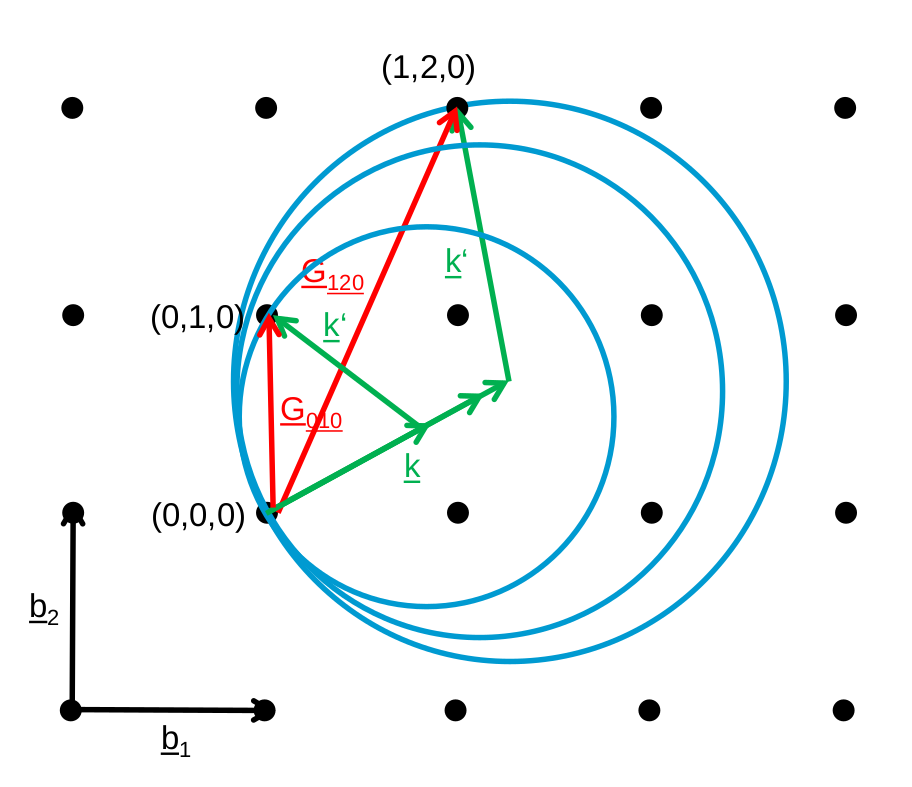
\includegraphics[width=0.7\textwidth]{figures/3_ewald.png}
		\caption{Ewald Konstruktion. Laue Verfahren (Vorlesungsfolie)}
		\label{}
	\end{figure}
\end{itemize}
\section{Gitterdynamik} \label{kap:4}
Physikalische Eigenschaften von FK bestimmt durch:
\begin{itemize}
	\item Bewegung der Atome von Gleichgewichtslage
	(Schallwellen, spezifische Wärme, Wärmeleitfähigkeit, thermische Ausdehnung etc.)
	\item Bewegung (fast freier) Elektronen (elektronische Eigenschaften)
\end{itemize}
Beide Phänomene sind nicht unabhängig. Hier: Born-Oppenheimer-Näherung (adiabatische Näherung):
\begin{itemize}
	\item Atomrümpfe bewegen aufgrund höherer Masse langsamer als Valenzelektronen.
	\item Verschiebung eines Atomrumpfs $\rightarrow$ 'instantane' Anpassung der Elektronenverteilung
	Dabei steigt Gesamtenergie des Elektronensystems Elektronen bleiben aber im Grundzustand (adiabatischer Prozess)
	\item Atome zurück in GG-Lage. Elektronensystem folgt und kehrt zur ursprünglichen Gesamtenergie zurück.
	\item Alles in allem: Bewegung der Atomrümpfe $\rightarrow$ Energieänderung des Elektronensystems. 
	$\rightarrow$ Potentialänderung der Atome (\textbf{Gitterdynamik}).
	Elektronen bleiben dabei im Grundzustand, und sind unabhängig von der Bewegung der Atomen $\rightarrow$ Beschreibung im
	ursprünglichem periodischen Potential. (\textbf{Elektronensystem} entkoppelt von Gitterdynamik)
\end{itemize}


\subsection{Potential in harmonischer Näherung}		\label{kap:4_1} 
Form des Potentials bestimmt durch Elektronensystem (kompliziert). \\
\textbf{Hier}: Qualitative Betrachtung: \\
Gesamtenergie des Kristalls $\Phi\left( \textbf{r}_{\textbf{n},\alpha} \right)$ hängt von Position 
der Atomrümpfe ($\textbf{n} = (n_1,n_2,n_3)$ Elementarzelle, $\alpha$ Basisposition). Auslenkung aus GG-Position 
$\textbf{r}_{\textbf{n},\alpha}$ sei $\textbf{u}_{\textbf{n},\alpha}$. \\
Taylorentwicklung: \\
% \begin{align}
% 	\Phi\left( \textbf{r}_{\textbf{n},\alpha,i} + \textbf{u}_{\textbf{n},\alpha,i}\right) = \Phi\left( \textbf{r}_{\textbf{n},\alpha,i} \right)
% 	 + \sum_{\textbf{n},\alpha,i} \frac{\partial \Phi}{\partial \textbf{r}_{\textbf{n},\alpha,i}}\vert_{\textbf{u}_{\textbf{n},\alpha,i} = 0\right)}
% 	 + \frac{1}{2} \sum_{\textbf{n},\alpha,i,\textbf{m},\beta,j} \frac{\partial^2 \Phi}{\partial \textbf{r}_{\textbf{n},\alpha,i} \partial \textbf{r}_{\textbf{m},\beta,j}}
% 	 \vert_{\textbf{u}_{\textbf{n},\alpha,i} = 0, \textbf{u}_{\textbf{m},\beta,j} = 0} \textbf{u}_{\textbf{n},\alpha,i} \textbf{u}_{\textbf{m},\beta,j}
% \end{align}

%TODO: Hier fehlt noch was

Atomrümpfe bewegen sich näherungsweise in harmonischem Potential.\\
Weitere Vereinfachungen:
\begin{itemize}
	\item[(i)] Wechselwirkung nur zwischen nächsten Nachbarn.
	(i.d.R. keine langreichweitige WW)
	\item[(ii)] Betrachtung einer 1D Kette von Atomen. (Modell der 1D Kette beschreibt Gitterdynamik eines 3D Kristalls gut)\\
	Ausbreitung einer ebenen Welle in Hochsymmetrierichtung:\\
	Aus Symmetriegründen kompensieren sich Kräfte, die nicht längs der Ausbreitungsrichtung wirken. Es treten entweder longitudinale oder transversale Moden (in Hochsymmetrierichtungen).\\
	\begin{itemize}
		\item[$\rightarrow$] Damit ist 3D Problem auf 1D Modell in Richtung des Wellenvektors zurückgeführt, da Netzebenen $\bot$  Wellenvektor die gleiche Bewegung.
		\item[$\rightarrow$] 1D Bewegungsgleichung mit effektiven Kräften, die Bewegung der gesamten Netzebene beschreiben.
	\end{itemize}
\end{itemize}



\subsection{Modell der linearen Kette} \label{kap:4_2}
\begin{itemize}
	\item[(a)] \textbf{Lineare Kette mit 1-atomiger Basis:}\\
	\begin{figure}[H]
		\centering
		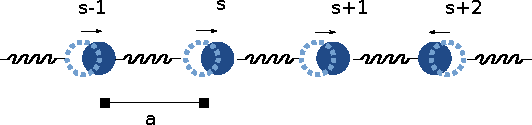
\includegraphics[width=0.8\textwidth]{figures/4_2linKette}
		\caption{}
		\label{}
	\end{figure}
	Rückstellkraft auf s-tes Atom: $F_s = c [(u_{s+1} - u_s) - (u_s - u_{s-1})]$
	Bewegungsgleichung
	\begin{align*}
		m \cdot\frac{\mathrm{d}^2 u_s}{\mathrm{d}t^2} &= c [(u_{s+1} - u_s) - (u_s - u_{s-1})]\\
		\text{Ansatz:} \qquad u_s &= U_0 \cdot e^{-i(\omega t + q s a)}\\
		\Rightarrow \qquad \qquad -\omega^2 \cdot m &= c [e^{-iqa} -1-1+e^{+iqa}]\\
		\omega^2 &= \frac{2 c}{m} [1 - \frac{1}{2} (e^{iqa} +e^{-iqa}]\\
		&= \frac{2 c}{m} (1- \cos(qa))\\
		&= \frac{4 c}{m} \sin^2\left(\frac{qa}{2}\right)
	\end{align*}
	$\Rightarrow$ Dispersionsrelation der linearen Kette: $\omega = 2 \cdot \sqrt{\frac{c}{m}}\left|\sin\left(\frac{qa}{2}\right)\right|$ \\
	\begin{figure}[H]
		\centering
		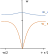
\includegraphics[width=0.4\textwidth]{figures/4_2disp}
		\caption{}
		\label{fig:4_2disrel}
	\end{figure}
	\textbf{Diskussion}: \\
	\begin{itemize}
		\item[(i)] Beschränkung des Wellenvektors auf die 1. Brillouin-Zone: \\
			Phasenunterschied 2er benachbarter Atome: $u_{s+1} / u_{s} = e^{iqa} = e^{i\varphi}$ ist maximal $2\pi$. 
			\begin{itemize}
				\item[$\rightarrow$] Betrachtung des Bereichs $-\pi < qa \le + \pi$  bzw.  $-\pi/a < q \le +\pi/a $ (1.BZ)
				\item[$\rightarrow$] Wellenvektor $q'$ außerhalb 1. BZ: Rücktransformation durch Addition eines geeigneten Gittervektors G
				\begin{align*}
					G = \frac{2 \pi}{a} \cdot p \quad (p \in \mathbb{Z})\text{, also} \quad q' = q + \frac{2 \pi}{a} \cdot p
				\end{align*}
				Begründung: $\frac{u_{s+1}}{u_{s}} = e^{iq'a} = e^{iqa}\cdot e^{i2\pi p} = e^{iqa}$
				\item[$\rightarrow$] Bei Rücktransformation in die 1. BZ kann Wellenvektor des Vorzeichen wechseln. Das entspricht einem VZ- Wechsel der Phasengeschwindigkeit $v_P = \omega / q$. Die Gruppengeschwindigkeit $v_G = \partial\omega / \partial q$ bleibt gleich ($\rightsquigarrow$ Energietransport der Welle).
			\end{itemize}
		\item[(ii)] \textbf{Grenzfälle:} \\
			\begin{itemize}
				\item[(I)] \textbf{Langwelliger Grenzfall:}\\
				$q \rightarrow 0$ bzw. $\lambda = 2 \pi / q \rightarrow \infty$
				\begin{align*}
					\omega \approx 2 \cdot \sqrt{\frac{c}{m}} \cdot \left| \frac{qa}{2} \right| \sim \left| q \right| 
				\end{align*}
				\begin{itemize}
					\item lineare Dispersion
					\item $v_p = \pm \sqrt{\frac{c}{m}}\cdot a $
					\item $v_G = \pm \sqrt{\frac{c}{m}} \cdot a $
				\end{itemize}
				\item[(II)] \textbf{Kurzwelliger Grenzfall:}\\
				$q \rightarrow \pm \pi / a$ bzw. $\lambda = 2 \pi / q \rightarrow 2a$
				\begin{align*}
					\omega \approx 2 \cdot \sqrt{\frac{c}{m}} \left(1-\frac{1}{2} \left( \frac{qa}{2} \right)^2\right) \approx 2 \cdot \sqrt{\frac{c}{m}}
				\end{align*}
				\begin{itemize}
					\item Dispersion $\approx$ konstant
					\item $v_p = \omega / q $, $V_G = \partial \omega / \partial q \to 0$ d.h \textbf{stehende Welle}
					\item relative Phasenlage: $u_{s+1} / u_s = e^{iqa} \quad \rightarrow \quad e^{\pm \pi} = -1$\\
					d.h. benachbarte Atome schwingen für $q \rightarrow \pm \pi / a$ gegenphasig. (stehende Welle mit $\lambda = 2a$)\\
					$\rightsquigarrow$ Auftreten der stehenden Welle kann als konstruktive Interferenz der einlaufenden Welle mit $ q = \pi / a $ und der gebeugten Welle verstanden werden: $ 2 \cdot a \cdot \sin(\theta) = n \cdot \lambda $ (für $n=1$, $\lambda = 2a$) \\
					$2 \cdot a \cdot \sin(\theta) = 2 \cdot a $, also $\theta = \ang{90}$ oder Streuwinkel $\ang{180}$.
					\begin{figure}[H]
						\centering
						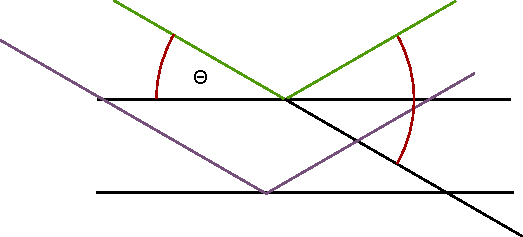
\includegraphics[width=0.4\textwidth]{figures/4_2winkel}
						\caption{}
						\label{fig:4_2winkel}
					\end{figure}
				\end{itemize} 
			\end{itemize}
	\end{itemize}
	\item[(b)] \textbf{Linear Kette mit 2-atomiger Basis:} \\
		Mit Federkonstante $c$ und Massen $m_A$, $m_B$.
		\begin{figure}[H]
			\centering
			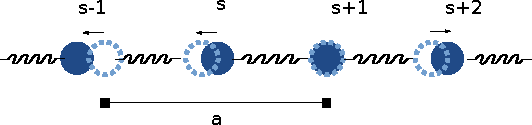
\includegraphics[width=0.8\textwidth]{figures/4_2Kette2}
			\caption{}
			\label{fig:4_2kette2}
		\end{figure} 
		Rückstellkraft:
		\begin{align*}
			F_{A,S} &= c \left[(v_s - u_s) - (u_s - v_{s-1})\right] \\
			F_{B,S} &= c \left[(u_{s+1} - v_s) - (v_s - u_{s})\right] 
		\end{align*}
		Bewegungsgleichungen:
		\begin{align*}
			m_A \cdot \frac{\mathrm{d}^2u_s}{\mathrm{d}t^2} &= c \cdot (v_s + v_{s-1} - 2 u_s) \\
			m_B \cdot \frac{\mathrm{d}^2v_s}{\mathrm{d}t^2} &= c \cdot (u_{s+1} + u_s - 2 v_s)
		\end{align*}
		Ansatz:
		\begin{align*}
			u_s &= U e^{-i(\omega t - q s a)} \\
			v_s &= V e^{-i(\omega t - q s a)}
		\end{align*}
		Ansatz einsetzen, Gleichungssystem lösen (Koeffizientendeterminante = 0):\\
		$\Rightarrow$ Dispersionsrelation:
		\begin{align*}
			\omega_{a,0}^2 = c \left( \frac{1}{m_A} + \frac{1}{m_A} \right) \mp c \sqrt{\left( \frac{1}{m_A} + \frac{1}{m_A} \right)^2 - \frac{4}{m_A m_B} \cdot \sin^2 \left(\frac{qa}{2}\right)}
		\end{align*}
		Maximum: $\tilde{\omega} = \omega_{max} = \sqrt{2c \left( \frac{1}{m_A} + \frac{1}{m_A} \right)} = \sqrt{\frac{2c}{\mu}}$
		\begin{figure}[H]
			\centering
			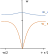
\includegraphics[width=0.4\textwidth]{figures/4_2disp}
			\caption{}
			\label{fig:4_2disp}
		\end{figure}
	\textbf{Diskussion:}\\
	\begin{itemize}
		\item[(A)] \textbf{Zweig $\omega_a$:}\\
		Wie lineare Kette mit 1-atomiger Basis ($m_A = m_B = m$ und $a \rightarrow 2a$)
		\begin{itemize}
			\item[(i)] Langwelliger Grenzfall: $q \rightarrow 0$ ($\lambda \rightarrow \infty$)
			\begin{itemize}
				\item lineare Dispersion
				\item relative Phasenlage benachbarter Atome: $\frac{u}{v} \approx \frac{2c}{2c-\omega_a^2 m_A} \approx 1$ (für $q \rightarrow 0$)\\
				d.h. benachbarte Atome schwingen $\approx$ gleichphasig mit fast gleicher Amplitude.
				% \begin{figure}[H]
				% 	\centering
				% 	\includegraphics[width=0.8\textwidth]{figures/4_2transWelle}
				% 	\caption{Visualisierung: Transversalwelle}
				% 	\label{fig:4_2transWelle}
				% \end{figure}
				$\Rightarrow$ im langwelligen Grenzfall verhalten sich die Gitterwellen wie Schallwellen: \textbf{akustischer Zweig} $\omega_a$.
			\end{itemize}
			\item[(ii)] Kurzwelliger Grenzfall: $q \rightarrow \pm \frac{\pi}{a}$ ($\lambda \rightarrow 2a$): $\omega_a^2 \rightarrow \frac{2c}{m_B}$ ($m_a < m_B$)
			\begin{itemize}
				\item konstante Dispersion
				\item relative Phasenlage $\frac{u}{v} = 0$\\
				d.h. das leichtere Untergitter A ist in Ruhe, das schwerere B schwingt. Benachbarte Atome B schwingen gegenphasig (vgl. (a)) %TODO ref?
			\end{itemize}
		\end{itemize}
		\item[(B)] \textbf{Zweig $\omega_0$:}
		\begin{itemize}
			\item[(i)] $q \rightarrow 0$ ($\lambda \rightarrow \infty$): $\omega_0^2 \approx 2c \left(\frac{1}{m_A} + \frac{1}{m_B}\right) = \frac{2c}{\mu} = \tilde{\omega}^2$
			\begin{itemize}
				\item konstante Dispersion
				\item $\frac{u}{v} \approx - \frac{m_B}{m_A}$
				% \begin{figure}[H]
				% 	\centering
				% 	\includegraphics[width=0.8\textwidth]{figures/4_2VisB}
				% 	\caption{Visualisierung (wie in (A))}
				% 	\label{fig:4_2VisB}
				% \end{figure} 
				d.h.gegenphasige Schwingung.\\
				Interpretation: Sind A, B Ionen mit unterschiedlichenLadungen entsteht ein oszillierendes elektrisches Dipolmoment. Damit koppeln Gitterschwingungen an elektromagnetischen Wellen (Infrarotbereich): \textbf{optischer Zweig} $\omega_0$.
			\end{itemize}
			\item[(ii)]  $q \rightarrow \pm \frac{\pi}{a}$ ($\lambda \rightarrow 2a$): $\omega_0^2 \rightarrow \frac{2c}{m_A}$ ($m_a < m_B$),\\
			d.h. für $m_A \neq m_B$ tritt Frequenzlücke auf, in der keine Gitterschwingungen existieren. Das Bedeutet Anregung ist $\omega$ im Bereich der Lücke klingen exponentiell ab.
			\begin{align*}
				-\frac{V}{U}\approx \frac{C(1+e^{\pm i\pi})}{2C-\omega_0^2m_B} = 0
			\end{align*}
			,d.h schwereres Untergitter B in Ruhe, A schwingt. Benachbarte Atome im A-Gitter Schwingen gegenphasig.
			\item[(iii)] Verallgemeinerung auf reale Kristalle:\\
			Betrache Ausbreitung in Symmetrierichtung in 3D-Kristall.\\
			Es treten longitudinale (L) oder transversale (T) Schwingungen auf.
		\end{itemize} 
		1-atomige Basis: 1L, 2T (senkrecht aufeinander, falls isotrop, entartet)\\
		\begin{itemize}
			\item[p-atomige Basis:]
			\begin{itemize}
				\item 3p Zweige
				\item 3 akustische (1L. 2T wie oben)
				\item 3p-3 optische ( (1p-1)L,  (2p-2)T )
			\end{itemize} 
		\end{itemize}
		z.B. 2-atomige Basis: 6 Zweige, 3 ak. (\textbf{1L}, 2T), 3 opt. (\textbf{1L}, 2T)
		% \begin{figure}[H]
		% 	\centering
		% 	\includegraphics[width=0.8\textwidth]{figures/4_2VisB.pdf}
		% 	\caption{zwischen -pi/a bis pi/a amplituden manche bei 0 min. manche max}
		% 	\label{fig:4_2VisC}
		% \end{figure}
	\end{itemize}
\end{itemize}




\subsection{Streuung an Kristallen mit Zeitlich veränderlichem Gitter} \label{kap:4_3}
 Aus Kap: \ref{kap:3_1} Streuamplitude,
\begin{align*}
	A_B(\Delta \textbf{k})= \underbrace{\frac{A_0}{R^i}e^{i(k'R+k'R')}}_{=: \tilde{\tilde{A}}} e^{i\omega_0t} \underbrace{\int \rho(\textbf{r})e^{-i\Delta kr} dr}_{\text{vgl. kap \ref{kap:3_3}}}
\end{align*}
\begin{itemize}
	\item[\textbf{Ann:}] Kristall mit 1-atomiger Basis (z.B. Neutronenstreuumg bisher)
	\item[\textbf{Jetzt:}] $\textbf{r} = \underbrace{\textbf{R}_n}_{\text{GG-Pos. des n-ten Atoms}} + \textbf{u}_n(t)$ Zeitabhängige Auslenkung des n-ten Atoms um GG-Lage.
\end{itemize}
\begin{align*}
	A_B(t) &= \tilde{\tilde{A}} e^{-i\omega_0 t} \sum_n \int \rho(\textbf{r}) e^{-i\Delta \textbf{k} \textbf{R}_n } e^{-i\Delta \textbf{k} \textbf{u}_n(t)} \mathrm{d}^3r\\
	&= \tilde{\tilde{A}} e^{-i\omega_0 t} \sum_n \rho_n e^{-i\Delta \textbf{k} \textbf{R}_n } e^{-i\Delta \textbf{k} \textbf{u}_n(t)} \text{für punktförmigen Streuer}
\end{align*}
Auslenkung der Gitterschwingung klein gegenüber a, d.h.$\Delta \textbf{k} \textbf{u}_n(t) \ll 1$, damit
\begin{align*}
	A_B(t) \approx \tilde{\tilde{A}} e^{-i\omega_0 t} \sum_n \rho_n e^{-i\Delta \textbf{k} \textbf{R}_n } \left(  1 -i\Delta \textbf{k} \textbf{u}_n(t) - \frac{1}{2}(\Delta \textbf{k} \textbf{u}_n(t))\right)
\end{align*}
Innere Entiwicklung:
\begin{align*}
	A_B(t) \approx \tilde{\tilde{A}} e^{-i\omega_0 t} \sum_n \rho_n e^{-i\Delta \textbf{k} \textbf{R}_n } - \tilde{\tilde{A}} e^{-i\omega_0 t} \sum_n \rho_n i\Delta \textbf{k} \textbf{u}_n(t) e^{-i\Delta \textbf{k} \textbf{R}_n}
\end{align*}
Ansatz: 
\begin{align*}
	\textbf{u}_n(t) = \sum_q \textbf{u}_q \cdot e^{\pm i(\textbf{q} \textbf{R} n - \omega_q t)}
\end{align*}
Überlagerung von ebenen Wellen mit $q > 0$.
\begin{align*}
	\rightarrow \quad A_B(t) \approx \underbrace{\tilde{\tilde{A}} e^{-i\omega_0 t} \sum_n \rho_n e^{-i\Delta \textbf{k} \textbf{R}_n }}_{\begin{matrix}
		\text{Beitrag elastischer Streuung}\\
		\text{vgl. Kap. \ref{kap:3_3}}\\
		\text{Wert } \neq 0 \text{ nur für }\\
		\Delta \textbf{k} = \textbf{G}_{hkl}
	\end{matrix}} - \underbrace{\tilde{\tilde{A}} e^{-i\omega_0 t} \sum_n \rho_n i\Delta \textbf{k} \textbf{u}_q e^{-i(\Delta \textbf{k} \mp \textbf{q}) \textbf{R}_n} e^{-i(\omega_0 \pm \omega_q) t}}_{\begin{matrix}
		\text{Beitrag inelastischer Streuung,} \\
		\text{geänderte Streubedingung:}\\
		\Delta \textbf{k} \mp \textbf{q} = \textbf{G}_{hkl} \text{ (Impulserhaltung)}\\
		\omega = \omega_0 \pm \omega_q \text{ (Energieerhaltung)}
	\end{matrix}}
\end{align*}

\subsection*{Inelastische Streuung eines Teilchens: Absorption eines Phonons}

\begin{align*}
	\hbar \omega &= \hbar \omega_0 \pm \hbar \omega_q\\
	\hbar \textbf{k'} &= \hbar \textbf{k} \pm \hbar \textbf{q} + \hbar \textbf{G}_{hkl}
\end{align*}

\subsection{Quantisierung von Gitterschwingungen}  \label{kap:4_4}

\begin{itemize}
	\item[bisher:] klassische Betrachtung, lineare Kette (hier: 1-atomige Basis) aus N Atomen.
	\item Jedes Atom: 3 Schwingungsmoden, insgesamt: 3N Normalmoden der kollektiven Bewegung der Atome
	\item Periodische Randbedingungen: $u_s \overset{!}{=} u_{s+N}$
	\begin{align*}
		\text{d.h.} \qquad u_0 e^{-i(\omega t + q \cdot s \cdot a)} &\overset{!}{=} u_0 e^{-i(\omega t + q \cdot s \cdot a + q \cdot N \cdot a)}\\
		\Leftrightarrow \qquad e^{-iqNa} \overset{!}{=} 1 \quad &\Leftrightarrow \quad q \overset{!}{=} \frac{2 \pi}{a} \cdot \frac{p}{N} \quad \text{mit} \quad p \in \mathbb{Z}
	\end{align*}
	für Wellenvektoren in der 1. BZ: $-\frac{N}{2} < p \leq + \frac{N}{2}$
	% \begin{figure}[H]
		% 	\centering
		% 	\includegraphics[width=0.8\textwidth]{figures/4_moden.png}
		% 	\caption{}
		% 	\label{fig:4_moden.png}
	% \end{figure}
	\begin{itemize}
		\item[$\rightarrow$] 3N Lösungen: Schwingungsmoden
	\end{itemize}
	Quantisierung: Jede Mode entspricht einem QM harmonischen Oszillator mit Energie $E_{q,j} = \hbar \omega_j(\textbf{q})(n_{qj} + \frac{1}{2})$ mit Wellenvektor \textbf{q} und $j$ = 1,2,3 Zweig-Index
\end{itemize}
\paragraph{Diskussion:}
\begin{itemize}
	\item[(1)] Bestimmter Schwingungszustand $\omega_j(\textbf{q})$ kann nur diskrete Energiewerte annehmen ($n_{qj} = 0,1,2,\dots$), je nach Besetzungszahl der Normalmode mit \textbf{q} im Zweig j.\\
	d.h. die Energie der Gitterschwingungen ist quantisiert.\\
	Welle-Teilchen-Dualismus: Das Quant der Gitterschwingung wird als \textbf{Phonon} bezeichnet.
	\begin{itemize}
		\item[$\rightarrow$] Gitterschwingung als quantisierte \textbf{Anregung der gesamten Kristalls} ODER
		\item[$\rightarrow$] Gitterschwingung als \textbf{Quasiteilchen} mit\\
		Energie $E_j(\textbf{q}) = \hbar \omega_j(\textbf{q})$\\
		Impuls $\textbf{p} ( \textbf{q}) = \hbar \textbf{q} = \hbar \textbf{q} + \hbar \textbf{G} $ (!Quasi-Impuls (Kristallimpuls)!)\\
		$\rightsquigarrow$ nur bis auf \textbf{G} festgelegt, d.h. Translationsinvarianz nur bzgl. \textbf{G}. (Physikalischer) Impuls des Kristalls
		\begin{align*}
			p &= m \cdot \frac{\mathrm{d}}{\mathrm{d}t} \sum_{\textbf{n} \alpha} u_{\textbf{n} \alpha} = m \cdot \frac{\mathrm{d}}{\mathrm{d}t} \sum_s u_0 e^{-i(\omega t + q  s a)}\\
			&= -i \omega m u_0 e^{-i \omega t} \sum_s e^{-i q s a} = -i \omega m u_0 e^{-i \omega t} \frac{1 - e^{-i q N a}}{1 - e^{-i q a}} \underset{\begin{matrix}
				\uparrow\\ 
				q = \frac{2 \pi}{a} \cdot \frac{p}{N}
			\end{matrix}}{=} 0
		\end{align*}
	\end{itemize}
\end{itemize}


\subsection{Experimentelle Bestimmung von Dispersionsrelationen} \label{kap:4_5}

Phononen (am Rand der 1. BZ):
\begin{align*}
	\lambda &\approx 2a \approx 3.6 \text{\AA}\\
	\nu &\approx 5 \text{THz}\\
	\hbar \omega &\approx 3.3 \cdot 10^{-21} \text{J} \approx 10^{-2} \text{eV}\\
	u &\approx 5 \cdot 10^{-23} \text{m}\\
	n_q &\approx 1.5 \cdot 10^{23} 1/\text{cm}^3 \approx N (\text{bei 300 K})
\end{align*}

\subsection*{Messung von Phononen:}
\begin{itemize}
	\item[(a)] \textbf{Kohärente inelastische Streuung mit Neutronen:}
	\begin{itemize}
		\item thermische Neutronen ($E \approx$ 100 meV)
		\item relative Energieänderung durch Phonon an BZ-Grenze
		\begin{align*}
			\frac{\delta E}{E} = \frac{10^{-2} \text{eV}}{10^{-1} \text{eV}} \approx \frac{1}{10}
		\end{align*}
	\end{itemize}
	\item[(b)] \textbf{Kohärente inelastische Röntgenstreuung}
	\begin{itemize}
		\item Röntgenlicht ($E \approx$ 10 keV) hat den deutlich kleineres
		\begin{align*}
			\frac{\delta E}{E} = \frac{10^{-2} \text{eV}}{10^{4} \text{eV}} \approx 10^{-6}
		\end{align*}
		d.h. Dispersion der Phononen ist experimentell schwer aufzulösen.
	\end{itemize}
	\item[(c)] \textbf{Lichtstreuung:}
	\begin{itemize}
		\item sichtbares Licht ($E \sim$ 100 meV) liefert
		\begin{align*}
			\frac{\delta E}{E} = \frac{10^{-2} \text{eV}}{10^{-1} \text{eV}} \approx \frac{1}{10}
		\end{align*}
		gut auflösbar, aber $\lambda \gg a$ (d.h. $k = \frac{2 \pi}{\lambda} \ll \frac{2 \pi}{a}$, also im Zentrum der 1. BZ)\\
		d.h. Phononendispersion, aber nur für $q$ = 0.\\
		Damit Formulierung Impulserhaltung nur in 1. BZ: $\textbf{k'} = \textbf{k} \pm \textbf{q}$
		\begin{itemize}
			\item[(i)] $q$ = 0: Streuung ohne Phononen. Rayleigh-Streuung
			\item[(ii)] $q \neq 0$: Streuung unter Emission/Absorption eines Phonons: Raman (o. Brillouin)-Streuung
		\end{itemize}
	\end{itemize}  
\end{itemize}



\subsection{Spezifische Wärmekapazität des Kristallgitters} \label{kap:4_6}

Definition (Thermodynamik):
\begin{align*}
	C_p = \left( \frac{\partial U}{\partial T} \right)_p \quad , \quad C_V = \left( \frac{\partial U}{\partial T} \right)_V
\end{align*}
$U$: Innere Energie, $p$: Druck, $V$: Volumen mit $C_p - C_V = \frac{9 \alpha^2}{\kappa} \cdot V \cdot T$ ($\alpha$: lineare thermische Ausdehnung, $\kappa$: Kompressibilität)\\
In Festkörpern ist $\alpha$ sehr klein, so dass $\underset{\begin{matrix}
	\uparrow\\
	Messung
\end{matrix}}{C_p} \approx \underset{\begin{matrix}
	\uparrow\\
	Theorie
\end{matrix}}{C_V}$\\
\begin{itemize}
	\item[Hier:] Beitrag von Gitterschwingungen zu $C_V$ $\rightarrow$ dielektrischer FK
	\item[Später:] Beitrag von Leitungselektronen zu $C_V$ $\rightarrow$ metallische FK 
\end{itemize}

\begin{itemize}
	\item[(a)] \textbf{Zustandsdichte der Phononen}
	\begin{itemize}
		\item Kristall ist (idealisiert) unendlich groß (Translationssymmetrie)\\
		$\rightarrow$ Gitterschwingungen: ebene Wellen, kontinuierliches \textbf{q}
		\item realer Kristall: $N$ Elementarzellen mit $p$ Atomen, also $p \cdot N$ Atome\\
		$\rightsquigarrow$ schwierig
		\item Lösung: periodische Randbedingungen: Für Auslenkungen 
		\begin{align*}
			&\qquad \textbf{u}(\textbf{r},t) = \textbf{U}_{\textbf{q}} e^{-i(\omega_q t - \textbf{q} \textbf{r})}\\
			&\text{mit} \qquad \textbf{u}(x,y,z,t) \overset{!}{=} \textbf{u}(x+L,y,z,t) \overset{!}{=} \textbf{u}(x,y+L,z,t) \overset{!}{=} \textbf{u}(x,y,z+L,t)\\
			&\Rightarrow \qquad e^{i q_x L} = e^{i q_y L} = e^{i q_z L} \overset{\begin{matrix}
				\text{für Kantenlänge $L$}\\
				!
			\end{matrix}}{=} 1\\
			&\Rightarrow\qquad q_i = \frac{2\pi}{L} \cdot m_i \quad \text{für} \quad i=1,2,3\qquad \text{mit}\quad-\frac{\sqrt[3]{N}}{2}<m_i \leq +\frac{\sqrt[3]{N}}{2}
		\end{align*}
		d.h. $q$ hat $(\sqrt[3]{N})^3 = N$ diskrete Werte für jeden Zweig, also insgesamt $3 \cdot p \cdot N$ Wellenvektoren (=Normalmoden)\\
		Es ist mit $\textbf{b}_i = \frac{2 \pi}{V_0} (\textbf{a}_j \times \textbf{a}_k)$:
		\begin{align*}
			\textbf{q} = \sum_{j = 1,2,3} \frac{m_i \cdot \textbf{b}_i}{\sqrt[3]{N}}
		\end{align*}
	\end{itemize} 


\textbf{Zustandsdichte im k-Raum}: Zahl der möglichen Zustände im reziproken Raum pro Volumen alle erlaubten q liegen in 1.BZ, damit
\begin{align*}
	D(q) = \frac{(\sqrt[3]{N})^3}{(2\pi)^3/V_0} = \frac{N \cdot V_0}{(2\pi)^3} = \frac{V}{(2\pi)^3}
\end{align*}
\textbf{NB}: analog für 2D und 1D:
\begin{align*}
	D^{2d}(q) &= \frac{(\sqrt{N})^2}{(2\pi)^2/A_0} = \frac{A}{(2\pi)^2} \\
	D^{1d}(q) &= \frac{N}{(2\pi)^2/L_0} = \frac{L}{(2\pi)^2}
\end{align*}

\textbf{Zustandsdichte im Frequenz-Raum}: Zahl der Zustände im Frequenzraum pro Volumen.\\
Bestimmung aud Dispersionsrelation:
% \begin{figure}[]
% 	\centering
% 	\includegraphics{figures/4_2gitter.pdf}
% 	\caption{Zustaende, dieser Frequenz zwischen $w(q)=\text{const}$} und $\omega+\mathrm(d)\omega=\text{const}$ liegen}
% 	\label{}
% \end{figure}

Integration (statt Summen, wegen grossen Zahlen von Atomen): $q(\omega+\mathrm{d}\omega)$

\begin{align*}
	\int_{\omega(q)=const}^{\omega+\mathrm{d}\omega = const} D(\omega)\mathrm{d}\omega = \int_{q(\omega)}^{q(\omega+\mathrm{d}\omega)} D(q)\mathrm{d}^3q
	= \frac{V}{(2\pi)^3}\int\mathrm{d}S_\omega\mathrm{d}q_\bot 
\end{align*}
wobei $ \mathrm{d}^3q = \mathrm{d}S_\omega \cdot \mathrm{d}q_\bot $ erstetzt wurde mit $\mathrm{d}S_\omega$ Flächenelement und $\mathrm{d}q_\bot$ Flächennormale.
Mit $v_g = \left|\frac{\mathrm{d}\omega}{\mathrm{d}q}\right| = \left|\text{grad}_q\omega\right| = \frac{\mathrm{d}\omega}{\mathrm{d}q_\bot} $ folgt
\begin{align}
	= \frac{V}{(2\pi)^3} \mathrm{d}\omega \int_{\omega = const} \frac{\mathrm{d}S_\omega}{\left|grad_q\omega\right|}
\end{align}
Damit:
\begin{align*}
	D(\omega) \mathrm{d} \omega \tilde{=} \int_{\omega(q)=const}^{\omega+\mathrm{d}\omega = const} D(\omega)\mathrm{d}\omega = \frac{V}{(2\pi)^3} \int \frac{\mathrm{d}S_{\omega}}{(\text{grad}_{q} \omega)} \mathrm{d}\omega
\end{align*}

$\rightarrow$ $D(\omega)$ ist hoch, wenn die Dispersionskurve flach ist.\\
Extremfall: $D(\omega)$ divergiert für $v_g = 0$ (van-Hore Singularitäten)\\
$\rightarrow$ für isotrope FK: Flächekonstanter Frequenz im rez. Raum $S_{\omega}$ ist Kugel mit Radius $|\textbf{q}|$:
\begin{align}
	\Rightarrow D(\omega) = \frac{V}{(2\pi)^3} \cdot \frac{4\pi q^2}{v_g} = \frac{V}{2\pi^2} \cdot \frac{q^2}{v_g}
\end{align}
\item[(b)] \textbf{Debye-Modell:}\\
\textbf{Annahmen:} \begin{itemize}
	\item[(1)] isotroper Festkörper
	\item[(2)] 1-atomige Basis (nur akustische Moden)
	\item[(3)] lineare Dispersion $\omega = c \cdot q$ (vgl. langwelliger Grenzfall) d.h. FK als elastisches Kontinuum mit Schallgeschwindigkeit $c$
	$$\Rightarrow D(\omega) = \frac{V}{2 \pi} \cdot \frac{\omega^2}{c^3}$$
	Gesamtzahl der Zustände: $\int_0^\infty D(\omega)\mathrm{d}\omega$ divergiert, Widerspruch zur Zahl von Phononenmoden pro Zweig. \\
	$\rightsquigarrow$ Trick: Abschneidefrequenz $\omega_{max}$\\
	\begin{align*}
		\int_0^{\omega_{max}} D(\omega)\mathrm{d}\omega &= \int_0^{\omega_{max}} \frac{V}{2 \pi^2} \frac{\omega^2}{c^3} = \frac{V}{6 \pi^2} \frac{\omega^3}{c^3} \overset{!}{=} N\\
		\Rightarrow \quad \omega_{max} &= \sqrt[3]{\frac{6 \pi^2 N}{V}} \cdot c
	\end{align*}
	Berücksichtigung aller 3 Zweige: $D(\omega)\mathrm{d}\omega = \frac{V}{2\pi^2} \underbrace{\left(\frac{1}{c_L^3} + \frac{2}{c_T^3}\right)}_{=: \frac{3}{c_D^3}} \omega^2\mathrm{d}\omega$\\
	mit der Debye-Geschwindigkeit $c_D$.

\item[(c)]\textbf{Mittlere thermische Energie eines Phonons:}
	statistische Physik: mittlere thermische Besetzung $<n>_T = \frac{1}{e^{\hbar\omega/k_BT}-1}$ (Bose-Einstein-Verteilungsfunktion)

\item[(d)]\textbf{Spezifische Wärmekapazität im Debye-Modell:}
	Beitrag Gitterschwingung zur inneren Energie
	\begin{align}
		U(T) &= \int_0^{\omega_p} \hbar\omega_{q,j} \cdot D(\omega_{q,j}) \cdot <n_{q,j}(\omega,T)> \mathrm{d}\omega = \frac{9N}{\omega_D^3} \int_0^{\omega_D} \frac{\hbar\omega_{q,j}^3\cdot\mathrm{d}\omega}{e^{\hbar\omega_{q,j}/k_BT}-1} \\
		\Rightarrow \quad C_V &= \left(\frac{\partial U}{\partial T}\right)_V = q N k_B \left(\frac{T}{\Theta}\right)^3 \cdot \int_0^{x_D} \frac{e^x x^4 \mathrm{d}x}{(e^x-1)^2}
	\end{align}
	mit $x = \frac{\hbar\omega_{q,j}}{k_BT}$ und $x_D = x(\omega=\omega_D)$ und $k_B\theta = \hbar\omega_D$.

\end{itemize}

\end{itemize}
\section{Elektronen im Festkörper} \label{kap:5}

Erinnerung adiabatische Näherung (Born-Oppenheimer-Näherung):\\
Elektronenbeugung und Gitterdynamik werden getrennt behandelt.
\begin{itemize}
    \item Bewegung der Valenzelektronen im \textbf{statischen} Potential des Gitters. (positiv geladene Ionenrümpfe)
    \item Bei Transportprozessen von Elektronen von Elektronen:
    Elektronen-Gitter-WW als Strömung betrachtet.
\end{itemize}

Weitere Vereinfachungen:
\begin{itemize}
    \item \textbf{Ein-Elektron-Näherung:} Betrachte einzelnes Elektron im statischen Potential gegeben durch Ionenrümpfe und alle anderen Elektronen.
    \begin{itemize}
        \item[$\rightarrow$] Vernachlässigung $e^-$-$e^-$-WW, die über statisches Potiential hinausgeht. Beispiel für $e^-$-$e^-$-WW: Magnetismus, Supraleitung.
    \end{itemize}
    \item Beachtung des Pauliprinzips: Zustände werden sukzessive aufgefüllt
    \begin{itemize}
        \item[$\rightarrow$] unabhängige Elektronen  
    \end{itemize}    
\end{itemize}

\subsection{Das freie Elektronengas} \label{kap:5_1}
Zunächst zusätzliche Vernachlässigung der Gitterperiodizität
\begin{itemize}
    \item[$\rightarrow$] einzelnes Elektron im konstanten Potentialtopf (Sommerfeld-Modell)
    \begin{figure}[H]
        \centering
        % GNUPLOT: LaTeX picture with Postscript
\begingroup
  \makeatletter
  \providecommand\color[2][]{%
    \GenericError{(gnuplot) \space\space\space\@spaces}{%
      Package color not loaded in conjunction with
      terminal option `colourtext'%
    }{See the gnuplot documentation for explanation.%
    }{Either use 'blacktext' in gnuplot or load the package
      color.sty in LaTeX.}%
    \renewcommand\color[2][]{}%
  }%
  \providecommand\includegraphics[2][]{%
    \GenericError{(gnuplot) \space\space\space\@spaces}{%
      Package graphicx or graphics not loaded%
    }{See the gnuplot documentation for explanation.%
    }{The gnuplot epslatex terminal needs graphicx.sty or graphics.sty.}%
    \renewcommand\includegraphics[2][]{}%
  }%
  \providecommand\rotatebox[2]{#2}%
  \@ifundefined{ifGPcolor}{%
    \newif\ifGPcolor
    \GPcolorfalse
  }{}%
  \@ifundefined{ifGPblacktext}{%
    \newif\ifGPblacktext
    \GPblacktexttrue
  }{}%
  % define a \g@addto@macro without @ in the name:
  \let\gplgaddtomacro\g@addto@macro
  % define empty templates for all commands taking text:
  \gdef\gplbacktext{}%
  \gdef\gplfronttext{}%
  \makeatother
  \ifGPblacktext
    % no textcolor at all
    \def\colorrgb#1{}%
    \def\colorgray#1{}%
  \else
    % gray or color?
    \ifGPcolor
      \def\colorrgb#1{\color[rgb]{#1}}%
      \def\colorgray#1{\color[gray]{#1}}%
      \expandafter\def\csname LTw\endcsname{\color{white}}%
      \expandafter\def\csname LTb\endcsname{\color{black}}%
      \expandafter\def\csname LTa\endcsname{\color{black}}%
      \expandafter\def\csname LT0\endcsname{\color[rgb]{1,0,0}}%
      \expandafter\def\csname LT1\endcsname{\color[rgb]{0,1,0}}%
      \expandafter\def\csname LT2\endcsname{\color[rgb]{0,0,1}}%
      \expandafter\def\csname LT3\endcsname{\color[rgb]{1,0,1}}%
      \expandafter\def\csname LT4\endcsname{\color[rgb]{0,1,1}}%
      \expandafter\def\csname LT5\endcsname{\color[rgb]{1,1,0}}%
      \expandafter\def\csname LT6\endcsname{\color[rgb]{0,0,0}}%
      \expandafter\def\csname LT7\endcsname{\color[rgb]{1,0.3,0}}%
      \expandafter\def\csname LT8\endcsname{\color[rgb]{0.5,0.5,0.5}}%
    \else
      % gray
      \def\colorrgb#1{\color{black}}%
      \def\colorgray#1{\color[gray]{#1}}%
      \expandafter\def\csname LTw\endcsname{\color{white}}%
      \expandafter\def\csname LTb\endcsname{\color{black}}%
      \expandafter\def\csname LTa\endcsname{\color{black}}%
      \expandafter\def\csname LT0\endcsname{\color{black}}%
      \expandafter\def\csname LT1\endcsname{\color{black}}%
      \expandafter\def\csname LT2\endcsname{\color{black}}%
      \expandafter\def\csname LT3\endcsname{\color{black}}%
      \expandafter\def\csname LT4\endcsname{\color{black}}%
      \expandafter\def\csname LT5\endcsname{\color{black}}%
      \expandafter\def\csname LT6\endcsname{\color{black}}%
      \expandafter\def\csname LT7\endcsname{\color{black}}%
      \expandafter\def\csname LT8\endcsname{\color{black}}%
    \fi
  \fi
    \setlength{\unitlength}{0.0500bp}%
    \ifx\gptboxheight\undefined%
      \newlength{\gptboxheight}%
      \newlength{\gptboxwidth}%
      \newsavebox{\gptboxtext}%
    \fi%
    \setlength{\fboxrule}{0.5pt}%
    \setlength{\fboxsep}{1pt}%
\begin{picture}(3968.00,2834.00)%
    \gplgaddtomacro\gplbacktext{%
      \csname LTb\endcsname%%
      \put(1210,704){\makebox(0,0)[r]{\strut{}$V_0 = 0$}}%
      \put(1210,2040){\makebox(0,0)[r]{\strut{}$E_{vac}$}}%
      \put(1342,484){\makebox(0,0){\strut{}0}}%
      \put(2679,484){\makebox(0,0){\strut{}$L$}}%
      \put(2902,2231){\makebox(0,0)[l]{\strut{}V(x)}}%
    }%
    \gplgaddtomacro\gplfronttext{%
      \csname LTb\endcsname%%
      \put(198,1658){\rotatebox{-270}{\makebox(0,0){\strut{}E}}}%
      \put(2456,154){\makebox(0,0){\strut{}x}}%
    }%
    \gplbacktext
    \put(0,0){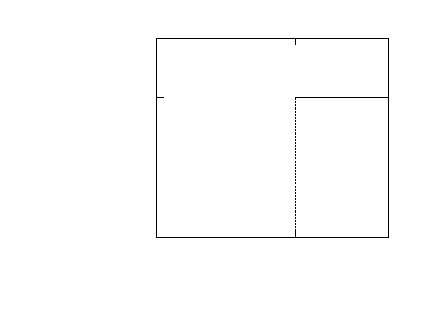
\includegraphics{figures/5_1Grapht}}%
    \gplfronttext
  \end{picture}%
\endgroup

        \label{5_1Graph}
    \end{figure}
    \item Beschreibung der Elektronen im Festkörper als \textbf{freies Elektronengas}
    \item Potentialtopf begrenzt durch Festkörper. Oberer Rand entspricht Vakuumzustnad (im Folgenden als $\infty$ angenommen)
    \item Gute Näherung für \glqq einfache Metalle\grqq (Alkalimetalle, Münzmetalle)
    \item Keine gute Näherung für die Übergangsmetalle
\end{itemize}

\begin{itemize}
    \item [(a)] \textbf{Schrödinger-Gleichung in 3D} \\
        \begin{align}
            \frac{-\hbar^2}{2m} \Delta \Psi(\textbf{r}) + V(\textbf{r}) \Psi(\textbf{r}) = E \Psi(\textbf{r})
        \end{align}
        mit Potential
        \begin{align*}
            V(\textbf{r}) = \begin{cases}
                0 & \text{für } 0 \le x,y,z \le L\\
                \infty & sonst
            \end{cases}
        \end{align*}
        Ansatz: Ebene Wellen $ \Psi(\textbf{r}) = \frac{1}{\sqrt{V}} e^{i\textbf{kr}}$  \\
        Energieeigentwert des Grundzustandes:
        \begin{align}
            E = \frac{\hbar^2k^2}{2m} = \frac{\hbar^2}{2m}(k_x^2 + k_y^2 + k_z^2)
        \end{align}
        Periodische Randbedingungen:\\ $\Psi(x,y,z) = \Psi(x+L,y,z) = \Psi(x,y+L,z) = \Psi(x,y,z+L)$ \\
        $\rightarrow$ $k_i = \frac{2\pi}{L} \cdot m_i $ mit $m_i$ für $i =x,y,z$ ganzzahlig. \\
        diskret aber \glqq liegen dicht \grqq d.h. quasikontinuierlich für große L. \\
        Für niedrigdimensionale Festkörper wird Schrödingergleichung mit Ansatz ebener Wellen für \glqq vorhandene Dimension \grqq und als stehene Welle für \glqq nicht vorhandene \grqq Dimension mit Wellenlänge $ \lambda_i = \frac{2d}{i} $. ($d$ : Abmessung in nicht vorhandener Dimension) \\
        
    \textbf{2D Zweidimensionales Elektronengas:} \\
    Z.B. dünne Metallfaden, 2DEG im Halbleiter-Heterostrah (Si-integrierte Schaltung) mit Dicke $d$
    \begin{align*}
        \lambda_i = \frac{2d}{i} \text{ oder } k_{i,z} = \frac{2\pi}{\lambda_i} = \frac{\pi}{d}i
    \end{align*}
    Schrödingergleichung mit
    \begin{align*}
        V(\textbf{r}) = \begin{cases}
                0 &\text{für } 0 \leq x,y \leq L\\
                \infty & \text{sonst}
            \end{cases}
    \end{align*}
    Ansatz 
    \begin{align*}
        \Phi(x,y,z) = \frac{1}{\sqrt{V}}\sin(k_z,it)\cdot e^{i k_x x}
    \end{align*}
    Eigenwerte
    \begin{align*}
        E = \frac{\hbar^2 k_{\Phi}^2}{2m} + \hbar^2 \frac{k_y^2}{2m} + \frac{i^2\hbar^2}{8md^2} \text{ mit } E_i = 8md^2
    \end{align*}
    Für $d\leq 5$mm werden tranversale Energien $E_i$ nicht vernachlässigt $\rightarrow$ 2D Subbänder: Parabeln in $k_x$- und $k_y$-Richtung.
    
    \textbf{2D Zweidimensionales Elektronengas:} \\
    1D Nanodraht mit quadratischen Querschnitt $\rightarrow$ Übungsauffgabe zu Lösen
    \begin{figure}[]
        \centering
        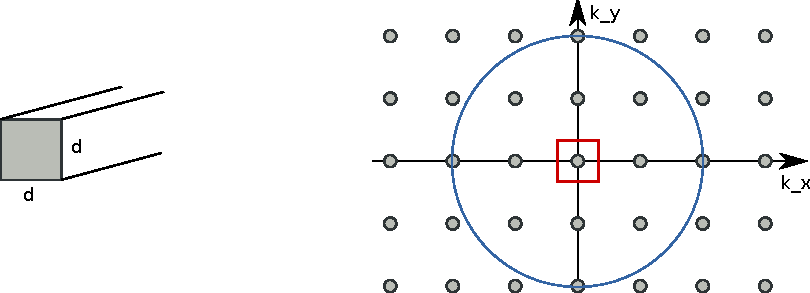
\includegraphics[]{figures/5_1Balken_Gitter.pdf}
        \caption{Die Dichte der erlaubten Wellenvektopren im k-Raum}
        \label{}
    \end{figure}
    \begin{itemize}
        \item 3D: $\delta^{3D}(k) = \frac{1}{\left(\frac{2\pi}{2}\right)} = \frac{V}{(2\pi)^3}$
        \item 2D: $\delta^{2D}(k) = \frac{A}{(2\pi)^2}$
        \item 1D: $\delta^{1D}(k) = \frac{L}{(2\pi)^1}$
    \end{itemize}
    \item[(b)] \textbf{Zustandsdichte} \\
        Zustandsdichte im Impulsraus: \\
        Die Dichte der erlaubten Wellenvektoren im k-Raum:
        \begin{align}
            3D \text{ : } \rho(k) &= \frac{1}{\left(\frac{2\pi}{L}\right)^3} &&= \frac{V}{(2\pi)^3} \\
            2D \text{ : } \rho(k) &= \dots &&= \frac{A}{(2\pi)^2} \\
            1D \text{ : } \rho(k) &= \dots &&= \frac{L}{(2\pi)^1}
        \end{align}
        Pauliprinzip: jeder k-Zustand kann doppelt besetzt werden wegen Spin: \\
        $\rightarrow$ $ 3D : D(k) = \frac{V}{(2\pi)^3} $ , $ 2D : \dots $  \\
        Zustandsdichte im Energieraum (analog zu Kap.4) in 3D:
        \begin{align}
            D(E)\mathrm{d} \approx \int_E^{E+\mathrm{d}E} D(E)\mathrm{d}E &= \int_{k(E)}^{k(E+\mathrm{d}E)} D(k)\mathrm{d}^3k = \frac{2V}{(2\pi)^3} \int_{k(E)}^{k(E+\mathrm{d}E)} \mathrm{d}^3k \\
            &= \frac{2V}{(2\pi)^3} \cdot 4 \pi k^2 \mathrm{dk}
        \end{align}
        wobei im letzten Schritt ausgenutzt wurde, dass $E = const$ auf Kugelfläche. \\
        Ausdrücken durch Energie: $ E = \frac{\hbar^2k^2}{2m} \rightarrow k = \sqrt{\frac{2mE}{\hbar^2}}$ und damit $ \frac{\mathrm{d}E}{\mathrm{d}k} = \frac{\hbar^2k}{m}$ \\
        $\rightarrow D(E) = \frac{V}{2\pi^2}\left(\frac{2m}{\hbar^2}\right)^{3/2}\sqrt{E} \propto \sqrt{E}$. \\
        \textbf{2D:} $D_i(E) = \frac{A}{2\pi}\frac{2m}{\hbar^2} = const $ ab $E \ge E_i$ \\
        $D^{2D}(E) = \sum_i D_i(E)$ \\
        \textbf{1D:} $D_{ij}(E) = \frac{L}{\pi}\left(\frac{2m}{\hbar^2}\right)^{1/2}\frac{1}{\sqrt{E}} \propto \frac{1}{\sqrt{E}} $ für $ E > E_{ij}$ \\
        $D^{1D}(E) = \sum_{i,j} D_{ij}(E)$
        \begin{figure}[H]
            \centering
            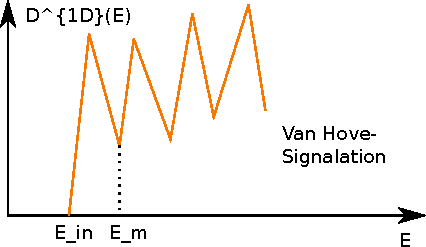
\includegraphics[]{figures/5_1zigzack.pdf}
            \caption{}
            \label{}
        \end{figure}
        
        Zustandsdichte und Dispersion des Fermigases
        % \begin{figure}[H]
        %     \centering
        %     \includegraphics[width=0.8\textwidth]{figures/5_zdfermi}
        %     \caption{}
        %     \label{fig:5_zdfermi}
        % \end{figure}

    \item[(c)] \textbf{Fermi-Energie}
    \begin{itemize}
        \item Betrachte System aus N nicht-ww Sl???????
        \item Füll Zustände aus (b) auf unter Beachtung des Pauliprinzips mit der Verteilunsfunktion $f(E,T)$, so dass gilt
        \begin{align}
            N = \int_0^\infty D(t) \cdot f(E,T) dE
            \label{eq:5_1_1}
        \end{align}
        Elektronengas (Fermi-Gas) bei T = 0:
        \begin{figure}[H]
            \centering
            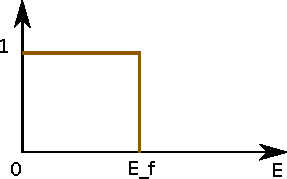
\includegraphics[]{figures/5_1Fermi.pdf}
            \caption{Fermi-Energie ist die Maximalenergie, bis zu der die Zustände bei $T=0$ konstant sind}
            \label{}
        \end{figure}
        \item Für drei Elektronen-Gase sind Flächen konstanter Energie Kugelflächen $\rightarrow$ $E_F^0$ entspricht Kugeloberfläche, die besetzte von unbesetzten Zuständen trennt.\\
         $k_F$ Fermikugelvektor
         \begin{align*}
             &N = \int_0^{E_F^0} D(E)dE = \frac{V}{2\pi^2} (\frac{2m}{\hbar^2})^\frac{3}{2}\frac{2}{3}(E_F^0)^\frac{3}{2}\\
             &\text{mit} \qquad n=\frac{N}{V} \text{ Elektronendichte}\\
            &\Rightarrow \qquad E_{F}^0 = \frac{\hbar^2}{2m} (3 \pi^2 n)^\frac{3}{2}
         \end{align*}
         \item[$\rightarrow$] hängt nur von Dimension und Elektronendichte ab
         \begin{itemize}
             \item[$\rightarrow$] Ein-Parameter-Modell
         \end{itemize} 
         $E_{F}^0 := \frac{\hbar^2 k_F^2}{2 m} \quad \rightarrow \quad k_F = ( 3 \pi^2 n )^{1/3}$ Fermi-Wellenvektor
         \begin{table}[H]
            \centering
             \begin{tabular}{ll}
                 Fermi-Geschwindigkeit & $v_F = \frac{\hbar k_F}{m}$\\
                 Fermi-Wellenlänge & $\lambda_F = \frac{2 \pi}{k_F}$\\
                 Fermi-Temperatur & $T_F = \frac{ E_F^0}{k_B}$\\
                 Zustandsdichte an der \glqq Fermi-Kante\grqq &
                    $D(E_F^0) = \frac{3}{2} \frac{N}{E_F^0}$ \\
                    &$\frac{D(E_F^0)}{V} = \frac{3}{2} \frac{n}{E_F^0}$
             \end{tabular}
         \end{table}

         Beispielwerte:
         \begin{table}[H]
             \centering
             \begin{tabular}{c|ccccc}
                 & $ n (10^{22}cm^{-3}) $ & $k_F ($\AA$^{-1})$ & $v_F (10^6 m/s)$ & $E_F^0 (eV)$ & $T_F (K)$  \\ \hline
            Li  & 4,62 & 1,11 & 1,1  & 4,69  & 54400 \\
            Na  &2,62   &0,91   &1,05   &3,11   &36700\\
            Al  &18,7   &1,75   &2,03   &11,67  &135700\\
            Ag  &5.87   &1.2    &1.39   &5.49   &62700 \\
            Au  &5,9    &1,2    &  1.38  &   5.51    &  63900    \\
                &       &$\approx \frac{1}{a}$  & $\approx 10^6 m/s$    & $\approx 5 eV $   & $T_F \gg T_{Schmelz} $ \\
                &       &                       & $< c$                 & $\gg k_BT$         & $> \Theta_D \approx RT $
            \end{tabular}
         \end{table}
    \end{itemize}
    \item[(ii)] \textbf{Elektronenegas bei endlicher Temperatur}
    \begin{align}
        f(E,T) = \frac{1}{e^{\frac{E-\mu}{K_B T}}}
    \end{align} 
    \begin{itemize}
        \item Energieintervall, in dem Umsetzungen möglich sind $\pm 1.75 k_B T$\\
            Da $k_B T_{TR} \approx 25 meV \ll E_F^0 $ ist Tieftemperaturnäherung of gerechtfertigt für Metalle.
        \item Für $T=0$ ist $\mu(T=0) = E_F^0$ 
        \item Mit N $\overset{!}{=} \int_0^{\infty} D(E) f(E,T) \mathrm{d}E \, \rightarrow \, \mu(T) \approx E_F^0 \left[1-\frac{\pi^2}{12} \left(\frac{T}{T_F}\right)^2 \right]$\\
            Für RT gilt in guter Näherung $\mu(300K) \approx E_F^0 = E_F$
    \end{itemize}


\item[(d)] \textbf{Spezifische Wärme des freien Elektronengases} \\
        Die innere Energie des Fermi-Gases bei $T=0$
        \begin{align}
            U_0 &= \int_0^\infty E D(E)f(E,T=0) \, \mathrm{d}E = \int_0^{E_F^0} E \frac{V}{2\pi^2} \left( \frac{2m}{\hbar^2} \right)^{3/2} \sqrt{E} \mathrm{d}E\\
            &= \frac{V}{2pi^2} \left(\frac{2m}{\hbar}\right)^{3/2} \cdot \frac{2}{5} (E_F^0)^{5/2} = \frac{3}{5} N \cdot E_F^0 = \frac{3}{5} N k_B T_F
        \end{align}
        Energiedichte $ n_0 = \frac{U_0}{V} = \frac{3}{5} n E_F^0 = \frac{3}{5} n k_B T_F$. \\
        Bei endlicher Temperatur
        \begin{align}
            U = \int_0^\infty E D(E) f(E,T) \mathrm{d}E = A\underbrace{\int_0^\infty \frac{E^{\frac{3}{2}}}{e^{\frac{E-\mu}{k_BT}}+1} \mathrm{d}E}_{\text{nicht analytisch lösbar}}
        \end{align}
        Spezifische Wärme $C_V = \left(\frac{\partial U}{\partial T}\right)_V$ \\
        \begin{itemize}
            \item[I] Abschätzung $\delta U(T) = U(T) - U_0$:
            \item[] {\centering
                \fbox{ $\delta U(T) \approx \underset{\text{Energiebetrag}}{k_B T} \cdot \underset{\text{Anzahl}}{N \frac{T}{T_F}} = N k_B \frac{T}{T_F} \, \rightarrow \, C_V = \left(\frac{\partial U}{\partial T}\right)_V = $}
                
            }


            \item[II] Rechnung \\
                Energieaufnahme des Fermi-Gases bei Erwärmung von $T=0$ auf T. \\
                \begin{align}
                    \delta U(T) = \int_0^\infty E D(E) f(E,T) \mathrm{d}E - \int_0^{E_F} E D(E) \mathrm{d}E \label{eq:5_1}
                \end{align} 
                Ferner
                \begin{align}
                    E_F N = E_F \int_0^\infty D(E) f(E,T) \mathrm{d} E \label{eq:5_2}
                \end{align}
                Leite \ref{eq:5_1} und \ref{eq:5_2} nach T ab.
                \begin{align}
                    C_v &= \int_0^\infty E D(E) \frac{\partial f(E,T)}{\partial T} \mathrm{d}E \label{eq:5_3} \\
                    0 &= E_F \int_0^\infty D(E) \frac{\partial f(E,T)}{\partial T} \mathrm{d}E \label{eq:5_4}
                \end{align} 
                Jetzt \ref{eq:5_3} - \ref{eq:5_3}:
                \begin{align}
                    C_v &= \int_0^\infty (E - E_F) D(E) \frac{\partial f(E,T)}{\partial T} \mathrm{d}E \\
                    &\approx D(E_F) \int_0^\infty (E - E_F) \frac{\partial f(E,T)}{\partial T} \mathrm{d}E
                \end{align}
                Wobei in der Abschätzung ausgenutzt wurde, dass $\partial f/\partial T \neq 0 $ nur um $E_F$. Mit
                \begin{align}
                    \frac{\partial f(E,T)}{\partial T} = \frac{E-E_F}{k_B T^2} \frac{e^{\frac{E-E_F}{k_BT}}}{\left(e^{\frac{E-E_F}{k_BT}} + 1\right)^2}
                \end{align}
                mit $x := \frac{E-E_F}{k_B T}$
                \begin{align}
                C_v = k_B^2 T D(E_F) \int_{-E_F / (k_B T) \rightarrow - \infty}^\infty \frac{x^2e^x}{(e^x+1)^2}\mathrm{d}x
                \end{align}
                {\centering
                \fbox{$ \frac{\pi^2}{3} k_B^2 T D(E_F) = \frac{\pi^2}{2} N k_B \frac{T}{T_F}$}
                }
        \end{itemize}
\begin{align*}
    C_V(T) = \underbrace{\gamma T}_{El.} + \underbrace{\beta T^3}_{Phonon} \qquad &\text{Gesamte spezifische Wärme}\\
    \frac{C_V(T)}{T} = \gamma + \beta T^2 \qquad &\text{geschickte Auftragung zur Best. von $\gamma$ und $\beta$}
\end{align*}
mit $\gamma := \frac{\pi^2}{2}N k_B \frac{1}{T_F}$, $\beta = \frac{12 \pi^4}{5} N k_B \frac{1}{\Theta_D^3}$.\\

\textbf{Diskussion:} \\
Für tiefe Temperaturen $(T \ll \Theta_D)$: Beitrag des Gitters recht kleine, da $T^3$-Abhängigkeit. $\rightarrow$ Anteil der Elektronen messbar (siehe Folie) wegen schwächerer T-Abhängigkeit. \\
Für hohe Temperaturen $(T \gg \Theta_D)$: Phononenbeitrag dominiert $C_{Ph} \approx 3 N_A k_B T$. \\
Bemerkung: \\
Modell passt gut ($\approx 25 \%$) für einfache Metalle, schlecht für Übergangsmetalle mit teilweise gefüllten d-Schalen.

\end{itemize}

\subsection{Elektronen im periodischen Potential} \label{kap:5_2}
Potential im Topf hat Translationssymmetrie des Gitters.
%TODO Bild 5_2
\begin{itemize}
    \item[(a)] \textbf{Bloch-Wellen:}\\
    Schrödingergleichung: $-\frac{\hbar^2}{2m} \Delta \Psi(\textbf{r}) + V(\textbf{r}) \Psi(\textbf{r}) = E \cdot \Psi(\textbf{r})$\\
    mit $V(\textbf{r}) = V(\textbf{r} + \textbf{R})$ mit Gittervektor $\textbf{R}$.\\
    Analog: Berechnung Streudichteverteilung $\rightarrow$ Fourier-Dartstellung $V(\textbf{r}) = \sum_{\textbf{G}} V_{\textbf{G}} e^{i \textbf{G} \textbf{r}}$ mit reziprokem Gittervektor $ \textbf{G}$. Die Fourierkoeffizienten $V_{\textbf{G}}$ sind charakteristisch für den Kristall. \\
    Ansatz für Wellenfunktion: Entwicklung nach ebenen Wellen
    \begin{align}
        \Psi(\textbf{r}) &= \sum_{\textbf{k}} c_{\textbf{k}} e^{i \textbf{k} \textbf{r}} = \sum_k \Psi_{\textbf{k}}(\textbf{r}) \\
        &=\sum_{\textbf{k}} \frac{\hbar^2 k^2}{2m} C_{\textbf{k}} e^{i \textbf{k} \textbf{r}} + \sum_{\textbf{k'},\textbf{G}} C_{\textbf{k'}} C_{\textbf{k}} e^{i (\textbf{k'} +\textbf{G}) \textbf{r}}\\
        &= E \sum_{\textbf{k}} C_{\textbf{k}} e^{i \textbf{k} \textbf{r}}
    \end{align}
    setzen $k := \textbf{k'} + \textbf{G} $ erlaubt, da über alle $\textbf{k}$, $\textbf{G}$ summiert wird. (entspricht Umsortierung).
    \begin{align}
        \sum_{\textbf{k}} e^{i \textbf{k} \textbf{r}} \left[\left(\frac{\hbar^2k^2}{2m} - E\right)c_{\textbf{k}} + \sum_{\textbf{G}} V_{\textbf{G}} c_{\textbf{k}-\textbf{G}}\right] \overset{!}{=} 0
    \end{align}
    für alle $\textbf{r}$. Somit
    \begin{align}
        \left(\frac{\hbar^2k^2}{2m} - E\right)c_{\textbf{k}} + \sum_{\textbf{G}} V_{\textbf{G}} c_{\textbf{k}-\textbf{G}} = 0
    \end{align}

    \begin{itemize}
        \item Satz algebraischer Gleichungen
        \item Zahl der erlaubten $\textbf{k}$ aus Randbedingungen
        \item Für jedes $\textbf{k}$ existiert ein Gleichungssystem mit Wellenfunktion $\Psi_{\textbf{k}}(\textbf{r})$ und Eigenwert $E_{k}$
        \item Genauso viele Lösungen wie $\textbf{k}$-Werte
        \item Entwicklungskoeffizienten $C_{\textbf{k}}$: ungleich 0, deren Indizes sich um $\textbf{G}$ unterscheiden.
    \end{itemize}

    \begin{align}
        \Psi_{\textbf{k}} (\textbf{r}) &= \sum_{\textbf{G}} c_{\textbf{k}-\textbf{G}} e^{i(\textbf{k}-\textbf{G}) \textbf{r}}\\
        \text{oder} \qquad \Psi_{\textbf{k}} (\textbf{r}) &= \underbrace{\left[\sum_{\textbf{G}} c_{\textbf{k}-\textbf{G}} e^{-i\textbf{G} \textbf{r}}\right]}_{
            \begin{matrix}
                \text{Fourierdarstellung einer} \\ \text{\textbf{R}-periodischen Funkion}\\
                u_{\textbf{k}} ( \textbf{r}) = u_{\textbf{k}} ( \textbf{r} + \textbf{R})
            \end{matrix}
        } e^{i \textbf{k} \textbf{r}}
    \end{align}
    
    $\rightarrow$ Elektronen im periodischen Potential sind Bloch-Wellen mit $u_{\textbf{k}}(\textbf{r}) = u_k(\textbf{r} + \textbf{R})$, $\Psi_{\textbf{k}} (\textbf{r}) = u_k(\textbf{r}) e^{i\textbf{k}\textbf{r}}$. \\
    Eigenschaften von Bloch-Wellen
    \begin{itemize}
        \item[(i)] Bloch-Wellen, die sich um $ \textbf{G} $ unterscheiden, sind identisch.
        \item[(ii)] Eigenwerte $E_{\textbf{k}}$ deren $ \textbf{k} $ sich um $ \textbf{G} $ unterscheiden, sind identisch. $\rightarrow$  $E_{\textbf{k}} = E_{\textbf{k}+\textbf{G}}$
        \item[(iii)]
        \begin{itemize}
            \item Die elektrischen Eigenschaften $\Psi_{\textbf{k}} (\textbf{r})$ und Eigenwerte $E_k$ wiederholen sich im $\textbf{k}$-Raum periodisch.
            \item Betrachtung in einer Einheitszelle des $\textbf{k}$-Raums ausreichend $\rightarrow$ 1. BZ.
        \end{itemize}
    \end{itemize}
    \item[(b)] \textbf{Modell des leeren Gitters}\\
    Annahme: Amplitude des periodischen Potentials so klein, dass dieser vernachlässigbar werden kann. $V_{\textbf{G}}\approx 0$, aber trotzdem Gitterperiodizität vorliegt.\\
    Aus (*) folgt: $ E_{\textbf{k}} = \frac{\hbar^2k^2}{2m} = \frac{\hbar^2}{2m} \left|\textbf{k}+\textbf{G}\right|^2 = E_{\textbf{k} + \textbf{G}}$ \\
    $\rightarrow$ Energieeigenwerte sind Parabeln im $\textbf{k}$-Raum, die sich um reziproken Gittervektor $\textbf{G}$ unterscheiden. \\
    \textbf{Beispiel}: 1D Gitter mit Gitterkonstante a, ausgedehnters Zonenschema \\ %TODO Bild 5.2b
    Reduziertes Zonenschema: Durch Verschieben der Parabeln von außerhalb in die 1. Bz (Addieren von $\textbf{G}$) \\ %TODO noch ein Bild 5.2c
    $\rightarrow$ zu jedem \textbf{k}-Vektor gibt es mehrere $E_k$. \\
    \textbf{Beispiel}: 3D kubisch primitives Gitter
    \begin{align}
        E_{\textbf{k}} = \frac{\hbar^2k^2}{2m} = \frac{\hbar^2}{m^2}\left[(k_x+G_x)^2 + (k_y+G_y)^2 + (k_z+G_z)^2\right] = E_{\textbf{k}+\textbf{G}}
    \end{align}
    \begin{itemize}
    \item[$\rightarrow$] 3D-Anordnung von Parabeln
    \item[$\rightarrow$] Auftreten von Entartung: vor allem bei hohen Energien fallen Parabeläste zusammen. $\rightarrow$ mehrere k-Zustände mit gleicher Energie im leeren Gitter
    \item[$\rightarrow$]] aufgehoben durch Hinzunahme eines endlichen Potentials $\rightarrow$ 
    \end{itemize}

    \item[(c)] \textbf{Modell fast freier Elektronen} \\
    Annahme: periodisches Potential so schwach, dass Elektronen sich nahezu frei durch den Kristall bewegen $\rightarrow$ gutes Modell für Leitungselektronen in Metallen, beschreibt das Auftreten von \textbf{Bandlücken}.
    \begin{itemize}
        \item[(i)] \textbf{Motivation:} Betrachte Bewegung eines Elektrons entlang 1D Atomkette. Elektron wir an Atomen gestreut: Bedingung für Bragg-Reflex: $\Delta \textbf{k} = \textbf{G}$. \\
        1D: Rückreflexion der einlaufenden Welle $\Delta \textbf{k} =  \textbf{k}' -  \textbf{k} = 2 \textbf{k} $. Auftreten der Bragg-Reflexion für $k = \pm G/2 = \frac{2\pi}{2a}\cdot n = \frac{\pi}{a} n \quad (n \in \mathrm{N}) \quad k_{min} = \frac{\pi}{a}$. \\
        In diesem Fall überlagern sich einlaufende und gestreute Welle zu stehender Welle
        \begin{align}
            \Psi_{s,a} \propto e^{i\pi \frac{x}{a}} \pm e^{-i\pi \frac{x}{a}} = \begin{cases}
                cos(\frac{\pi x}{a}) & \text{für } s \\
                sin(\frac{\pi x}{a}) & \text{für } a 
            \end{cases}
        \end{align}
        $\rightarrow$ Räumlich modulierte Ladungsdichte:
        \begin{align}
            \rho_{s,a} = e \left|\Psi_{s,a}\right|^2 \propto \begin{cases}
                cos(\frac{\pi x}{a}) & \text{für } s \\
                sin(\frac{\pi x}{a}) & \text{für } a 
            \end{cases}
        \end{align}
        (vergleich laufende ebene Welle ist räumlich konstant.)\\
        Braggreflexion am Rand der 1. BZ für $k_{???} = \pm \frac{\pi}{a}$\\
            $\rightarrow$ stehende Welle mit $\rho_s$ und $\rho_a$.\\
            $\rho_{s,a}$ hat hohe/niedrige Ladungsdichte an Ort der Inonen. Gesamtenergie für $\Psi_{s,a}$ niedriger/höher\\
            $\rightarrow$ Aufspaltung in ??? \textbf{Energiebänder} durch Aufhebung der Entartung $E_{s,a}$ abgesenkt/erhöht.  
            \item[(ii)] \textbf{Berechnung der Energielücke am Rand der BZ:}\\
            \begin{itemize}
                \item Rand der BZ ($k = \frac{\pi}{a}$) Schnittpunkt zweier Energieparabln: $E_{\textbf{k}}$ und $E_{\textbf{k}-\textbf{G}_0}$
                \item Schwaches Potential: Zwei-Komponenten-Näherung: 1. und 2. BZ reicht aus.
                \begin{align*}
                    \Psi(\textbf{r}) = c_{\textbf{k}} e^{i \textbf{k} \textbf{r}} + c_{\textbf{k}-\textbf{G}_0} e^{i(\textbf{k}-\textbf{G}_0) \textbf{r}}
                \end{align*}
                Aus (???) zur ??? Gleichungen
                \begin{align*}
                    \left(\frac{\hbar^2 k^2}{2m}-E\right) c_{\textbf{k}} + V_{\textbf{G}_0} c_{\textbf{k}-\textbf{G}_0} &= 0\\
                    \left(\frac{\hbar^2 \left|\textbf{k}-\textbf{G}_0\right|^2}{2m}-E\right) c_{\textbf{k}-\textbf{G}_0} + V_{-\textbf{G}_0} c_{\textbf{k}} &= 0
                \end{align*}
                mit dem Inversionssymmetrischen Filter $V_{-\textbf{G}_0} = V_{\textbf{G}_0}$.\\
                Lösung liefert
                \begin{align*}
                    E_{s,a} = E_{\textbf{k}}^0 \mp \left|V_{\textbf{G}_0} \right| \, , \quad E_a-E_s=2 \left|V_{\textbf{G}_0}\right|
                \end{align*}
                Verlauf der Dispersion am Rand der BZ: $E_{s,a} \sim \pm \left| k - \frac{G_0}{2} \right|^2$\\
                \begin{itemize}
                    \item[$\rightarrow$] negative Krümmung von $\Psi_s$ entspricht negativer Masse.
                    \item Tief in BZ keine Änderung, Änderungen am Rand der BZ.
                    \item Auftreten von Energiebändern (erlaubte Energiebereiche) und dazwischen Bandlücke (verbotener Energiebereich)
                    \item ???
                \end{itemize}
            \end{itemize}
        \end{itemize}
    \item[(d)] \textbf{Modell stark gebundener Elektronen (Tight binding Modelle)} \\
    \textbf{Annahme:} Es sei in der Nähe der Atomrümpfe lokalisiert. Beschreibung der Zustände durch Atomorbitale (Linear Combination of Atomic Orbitals / LCAO) (vgl. Bindungstypen).\\
    \begin{itemize}
        \item Ein-Elektron-Näherung Gitterpotential als Summe der Atompotentiale $V_A(r)$ Potential des Bezugatoms und ein Störpotential durch alle anderen Kristallatome
        \item Energieeigenwerte aus Rityschem Verfahren \begin{align*}
            E_{\textbf{k},i} = \frac{\int \Psi_{\textbf{k},i}^* H \Psi_{\textbf{k},i} \mathrm{d}r}{\int \Psi_{\textbf{k},i}^* \Psi_{\textbf{k},i} \mathrm{d}r}
        \end{align*}
        ist angenäherte Wellenfunktion.
        \begin{align*}
            \Psi_{\textbf{k},i}\approx \Phi_k = \underset{\begin{matrix}
                \uparrow\\
                \text{Anzahl}\\
                \text{Atome}
            \end{matrix}}{\frac{1}{\sqrt{N_A}}}\sum_m \underset{\begin{matrix}
                \uparrow\\
                \text{atomare}\\
                \text{Wellenfkt.}
            \end{matrix}}{\Psi^0_i(\textbf{r}-\textbf{R}_m)}\cdot \underset{\begin{matrix}
                \uparrow\\
                \text{Blochwellen}
            \end{matrix}}{e^{i \textbf{k} \textbf{R}_m}}
        \end{align*}
        \item Annahme: einfach kubisch, 1-atomige Basis,nächste Nacharn 
        \begin{align*}
            E_{k,i} \approx  \underset{\begin{matrix}
                \text{Eigentwert des}\\
                \text{isolierten Atom}           \end{matrix}}{E_i} - A_i - 2B_i[\cos(k_x a)+ \cos(k_y a) + \cos(k_z a)]
        \end{align*}
        \begin{table}[H]
            \begin{tabular}{cc}
                $E_i$ & Eigentwert des isolierten Atom\\
                $A_i$ & ??? \\
                $B_i$ & durch Überlapp der Wellenfunktion $\int \Psi^* \Psi \mathrm{d}r$
            \end{tabular}
        \end{table}
        \begin{itemize}
            \item[(1)] Wechselwirkung der  $N_A$ Atome $\rightarrow$ Aufspaltund der Energieniveaus in $N_A$ quasikontinuirliche Zustände, aus diskreten Energien werden \textbf{Energiebänder}.
            \item[(2)] Mittlere Verschiebung des Energieniveaus i (Lage der Bandmitte ist $A_i$: $A_i > 0$ $\rightarrow$ Absenkung
            \item[(3)] $A_i$ durch Potential der Nachbaratomre, nimmt zu für abnehmenden Gitterabstand a, Absenkung am stärksten für klein a.
            \item[(4)] Btreite des Bandes ist $\alpha$ $B_i$. Für sc: Bandbreite $\pm 6 B_i$
            \item[(5)] $B_i$ bestimmt durch Überlappintegral, Tiefliegende Zustände haben schmale Bänder, da Überlapp gering
            \item[(6)] In der Mitte der BZ ($\textbf{k} = 0$). $E_{k,i} (k) = E_i A_i - 6 B_i + B_i a^2k^2$
            $\rightarrow$ näherungsweise quadratische Dispersion\\
            mit effektiver Masse $m_i^* = \frac{\hbar^2}{\sum B_i a^2}$ durch Überlapp der Wellenfkt.
            \item[(7)] Bandindex an Atomorbitalen
            \item[(8)] Jedes Band kann gemäß Pauliprinzip $2N_A$ Elektronen aufnehmen 
        \end{itemize}
    \end{itemize}
\end{itemize}

\section{Elektronische Transporteigenschaften} \label{sec:6}
In Kapitel 5: Stationäre SGL im TD GG $\rightarrow$ elektronische Zustände im Gitter. \\
Hier: Bewegung von Elektronen im Festkörper, z.B
\begin{itemize}
    \item elektrische Leitfähigkeit
    \item Wärmeleitfähigkeit
\end{itemize}
$\rightarrow$ zeitabhängige Probleme, System nicht im TD GG durch Anlgegen von äußeren Feldern (elektrisch o. magnetisch).

\subsection{Semiklassische Bewegungsgleichung von Ladungen in Bändern} \label{sec:6_1}
bisher: Elektronen als ausgedehnte Wellen (Bloch-Wellen) \\
hier: lokalisierte Elektronen für Transport:
\begin{itemize}
    \item Unschärferelation ($\Delta p \cdot \Delta x \ge \hbar$ oder $\Delta k \cdot \Delta x \ge 1$), d.h. räumliche Lokalisierung bedingt Unbestimmtheit des Wellenvektors.
    \item \textbf{freie Elektronen}: lineare Superposition von ebenen Wellen mit $k - \Delta k / 2 < k < k + \Delta k / 2$ führt auf \textbf{Wellenpakete}
          \begin{align}
              \Psi(\textbf{r},t) \propto \int_{k-\Delta k/2}^{k+\Delta k/2} a(\textbf{k}) e^{i(\textbf{k}\textbf{r} - \omega(\textbf{k})t)} \mathrm{d}\textbf{k}
          \end{align}

          \begin{figure}[H]
              \centering
              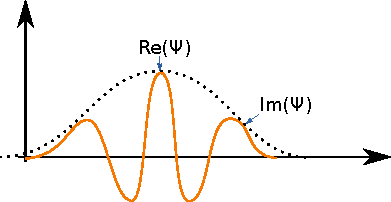
\includegraphics[width=0.8\textwidth]{figures/6_1Welle.pdf}
              \caption{}
              \label{fig:6_1Welle}
          \end{figure}

          Schwerpunkt des Pakets bewegt sich mit Gruppengeschwindigkeit $v_G = \left|\frac{\partial\omega(\textbf{k})}{\partial k}\right|$.
    \item \textbf{Im Kristall}: Superposition von Bloch-Wellen zu Wellenpaket: \\
          Wieder muss Unschärferelation gelten. Zusätzlich muss $\Delta k \ll \frac{\pi}{a}$ gelten, oder $\Delta x \gg a$, d.h. Wellenpaket dehnt sich über mehrere Elementarzellen aus. Bewegung des Elektrons (Wellenpakets) im äußeren Feld $\rightarrow$ Wellenlänge des Feldes $\lambda >> \Delta x$.

          \begin{figure}[H]
              \centering
              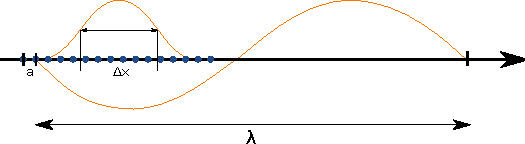
\includegraphics[width=0.8\textwidth]{figures/6_2BewEl.pdf}
              \caption{}
              \label{fig:6_1BewEl}
          \end{figure}

          Gruppengeschwindigkeit für das n-te Band: $\textbf{v}_n(\textbf{k}) = \nabla_\textbf{k} \omega(\textbf{k}) = \frac{1}{\hbar} \frac{\partial E_n(\textbf{k})}{\partial \textbf{k}} $ \\
          vorgehen: zeitabhängige SGL für nicht zu starke äußere Felder (vgl mit atomaren Feldern), die nicht zu stark räumlich und zeitlich variieren. $\rightarrow$ Theoretische Festkörperphysik \\
          hier: Semiklassische Bewegungsgleichung:
          \begin{align}
              \hbar \dot{\textbf{k}} = \textbf{F} = -e\left[\textbf{E}(\textbf{r},t) + \textbf{v}_n(\textbf{k}) \times \textbf{B}(\textbf{r},t)\right]
          \end{align}

          Analog zur Bewegungsgleichung freier Elektronen, aber mit $\textbf{v}_n(\textbf{k})$ und mit Quasiimpuls $\hbar \textbf{k}$ (nur bis auf $\textbf{G}$ festgelegt). Damit:
          \begin{align}
              \dot{\textbf{v}}_n = \frac{\partial}{\partial t} \left( \frac{1}{\hbar} \frac{\partial E_n(\textbf{k})}{\partial \textbf{k}} \right) =  \frac{1}{\hbar} \frac{\partial}{\partial \textbf{k}} \left( \frac{1}{\hbar} \frac{\partial E_n(\textbf{k})}{\partial \textbf{k}} \right) \cdot \hbar \cdot \frac{\partial \textbf{k}}{\partial t} = \frac{1}{\hbar^2} \frac{\partial^2 E_n(\textbf{k})}{\partial \textbf{k}^2} \cdot \textbf{F}
          \end{align}
          mit der inversen Masse $m\dot{v} = F$. \\
          \textbf{Definition:} \textbf{effektive Masse} $m^*$
          \begin{align*}
              \left(\frac{1}{m^*_n}\right)_{ij} (\textbf{k}) = \frac{1}{\hbar^2}\frac{\partial E_n(\textbf{k})}{\partial k_i\partial k_j} \\
              \text{mit $i,j$ = 1,2,3}
          \end{align*}

          \begin{itemize}
              \item Tensor
              \item Die inverse effektive Masse $\sim$ Krümmung der Energiedispersion des n-ten Bandes
              \item \textbf{k}-Abhängigkeit
              \item Wechselwirkung zwischen Elektron und Kristallpotential steckt in $m^*$: \\
                    BWGL: $\underline{\underline{m_n^*}} \cdot \dot{\textbf{v}}_n = \textbf{F}_i$ Impuls: $\underline{\underline{m_n^*}} \cdot \textbf{v}_n = \hbar \textbf{k}$ \\
                    d.h bei Kristallelektronen hängt Beschleunigung i.d.R von \textbf{k} ab, und Beschleunigung und Kraft müssen nicht parallel sein. \\
                    Für $\underline{\underline{m_n^*}}$ gilt: \\
              \item Tensor ist symmetrisch, d.h. $(\underline{\underline{m_n^*}})_{ij} = (\underline{\underline{m_n^*}})_{ji}$ bzw. für die Inversen.
              \item Tensor lässt sich auf Hauptachsen transformieren $\rightarrow$ 3 unabhängige Komponenten.\\
                    Spezialfälle:
                    \begin{itemize}
                        \item[1] effektive Masse längs Hauptachsen gleich groß $\rightarrow$ isotrope elektronische Eigenschafen
                        \item[2] quadratische Dispersion des Bandes $E_n(\textbf{k}) = E_0 + \frac{\hbar^2}{2m_n^*}(k_x^2 + k_y^2 + k_z^2)$ $\rightarrow$  konstantes $m_n^*$ ($\rightarrow$  in der Nähe der Bandextrema !)
                    \end{itemize}
              \item $m_n^* (\textbf{k})$ für isotropen Festkörper
              \item $m_n^*$ für Band mit quadratischer Dispersion
                    \begin{itemize}
                        \item[$\rightarrow$] in der Nähe der Bandextrema lassen sich Energieniveaus i.d.R. gut durch Paraboloide beschreiben
                        \item[$\rightarrow$] $m_n^*$ kann positiv oder negativ sein.
                              % \begin{figure}[H]
                              %     \centering
                              %     \includegraphics[width=0.8\textwidth]{figures/6_m_eff.png}
                              %     \caption{($\rightsquigarrow$ Krümmung des Bandes)}
                              %     \label{fig:6_m_eff.png}
                              % \end{figure}
                    \end{itemize}
          \end{itemize}
\end{itemize}



\subsection{Elektronen und Löcher} \label{sec:6_2}
Was ist Beitrag der Elektronen aus \textbf{einem} Band zur Stromdichte:
\begin{itemize}
    \item[Ann.:] Keine Interbandübergänge, d.h. angelegte Felder sind nicht stark genug, um das Band zu ändern ($n$ = const)
\end{itemize}
Stromdichte (Strom pro Quadratschnittsfläche)
\begin{align*}
    \mathrm{d}\textbf{j}_{(n)} = \frac{D(k)}{V} (-e \cdot v(\textbf{k})) \cdot \mathrm{d}^3k
\end{align*}
mit $e$ = \SI{1.6}{\cdot 10^{-19} C} und $D(k) = \frac{2V}{(2 \pi)^3}$ (vgl. Kap. \ref{kap:5_1}).
\begin{align*}
    \textbf{j}_{(n)} = -\frac{e}{V} \int D(k) \cdot f(E(\textbf{k}),T) \cdot \textbf{v}(\textbf{k}) \mathrm{d}^3k
\end{align*}
Ann.: $T$ = \SI{0}{K}, $f(E(\textbf{k}),T) = \Theta(E_F^0 - E(\textbf{k}))$ mit der Fermi-Energie $E_F^0$.
\begin{align*}
    \Rightarrow \quad \textbf{j}_{(n)} = - \frac{e V}{4V\pi^3} \int_0^{\textbf{k}E_F^0} \textbf{v}(\textbf{k}) \mathrm{d}^3k = - \frac{e}{4 \pi^3} \int_0^{\textbf{k}E_F^0} \frac{1}{\hbar} \underset{\begin{matrix}
        \uparrow \\
        \nabla_k E(\textbf{k})
    \end{matrix}}{\frac{\partial E (\textbf{k})}{\partial\textbf{k}}} \mathrm{d}^3k
\end{align*}

\begin{itemize}
    \item[(a)] \textbf{Vollständig besetztes Band:} \\
        $\rightarrow$ Integration über gesamte 1.BZ: \\
        Aus Symmetriegründen ist $\textbf{j} = 0$, d.h \textbf{vollständig besetzte Bänder tragen nicht zum Ladungstransport bei}. \\
        Begründung:
        \begin{itemize}
            \item[(i)] Kristall mit Inversionssymmetrie $E(\textbf{k}) = E(- \textbf{k})$ \\
                \begin{align}
                    \textbf{v}(\textbf{k}) = \frac{1}{\hbar} \frac{\partial E(\textbf{k})}{\partial \textbf{k}} = \frac{1}{\hbar} \frac{\partial E(-\textbf{k})}{\partial \textbf{k}} = - \textbf{v}(-\textbf{k})
                \end{align}
            \item[(ii)] Kristall ohne Inversionssymmetrie:\\
            Zeitumkehrinvarianz der SGL: $E(\textbf{k},\uparrow) = E(-\textbf{k},\downarrow) $, damit für $\uparrow$ und $\downarrow$ Elektronen $\textbf{v}(\textbf{k}) = - \textbf{v}(-\textbf{k})$
        \end{itemize}
    \item[(b)] \textbf{teilweise besetzes Band:}
        \begin{align}
            \textbf{j} &= \textcolor{red}{-} \frac{e}{4\pi^3} \underset{\begin{matrix}
                \text{\textcolor{red}{unbesetzte}}\\
                \text{\textcolor{red}{Zustände}}
            \end{matrix}}{\int} \frac{\partial E(\textbf{k}) }{\partial \textbf{k}} \mathrm{d}^3 k\\
             &= \frac{e}{4\pi^3} \left[    \underbrace{\int_\text{1. BZ} \frac{1}{\hbar} \frac{\partial E(\textbf{k}) }{\partial \textbf{k}} \mathrm{d}^3 k }_{=0}   -  \underset{\begin{matrix}
                \text{unbesetzte}\\
                \text{Zustände}
            \end{matrix}}{\int} \frac{1}{\hbar} \frac{\partial E(\textbf{k}) }{\partial \textbf{k}} \mathrm{d}^3 k \right] \\
             &= + \frac{e}{4 \pi^3} \underset{\begin{matrix}
                \text{unbesetzte}\\
                \text{Zustände}
            \end{matrix}}{\int} \frac{1}{\hbar} \frac{\partial E(\textbf{k})}{\partial \textbf{k}} \mathrm{d}^3 k = \textcolor{blue}{+} \frac{e}{4 \pi^3} \underset{\begin{matrix}
                \text{\textcolor{blue}{unbesetzte}}\\
                \text{\textcolor{blue}{Zustände}}
            \end{matrix}}{\int} \frac{1}{\hbar} \textbf{v}(\textbf{k}) \mathrm{d}^3 k\\
            &\neq 0 \quad \text{falls } \textbf{E} \text{ oder } \textbf{B} \text{ Feld anliegt, also System nicht in TD GG ist.}
        \end{align}
        $\rightsquigarrow$  mit 2 Betrachtungsmöglichkeiten
        \begin{itemize}
            \item[\textcolor{red}{\textcircled{1}}] Transport in teilweise gefüllten Bänderen wird von \textcolor{red}{Elektronen} auf \textcolor{red}{besetzten} Zuständen getragen. \textcolor{red}{$\rightsquigarrow$ für fast alle Bänder}
            
            \item[\textcolor{blue}{\textcircled{2}}] Transport in teilweise gefüllten Bändern wird von positiven Ladungsträgern \textcolor{blue}{(Defektelektronen, Löcher)} auf den mit Elektronen unbesetzten Zuständen getragen. $\rightsquigarrow$ fast volle Bänder
        \end{itemize}
        Nahe des Bandmaximums:
        \begin{figure}[H]
            \centering
            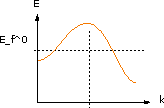
\includegraphics[width=0.5\textwidth]{figures/6_3Band.pdf}
            \caption{}
            \label{fig:6_3Band}
        \end{figure}
        \begin{align*}
            E(k) \approx E(k_0) + \frac{1}{2} &\underbrace{ \frac{\mathrm{d}^2E}{\mathrm{d}k^2}} (k-k_0)^2 \\
            &= \frac{\hbar^2}{m_e^*} = -\frac{\hbar^2}{|m_e^*|} (m_e^* < 0)
        \end{align*}
        damit:
        \begin{align*}
            \textbf{v}(\textbf{k}) &= \frac{1}{\hbar} \left(-\frac{\hbar^2}{|m_e^*|}(\textbf{k}-\textbf{k}_0)\right) \\
            \dot{\textbf{v}}(\textbf{k}) &= - \frac{\hbar \dot{\textbf{k}}}{|m_e^*|} \approx - \dot{\textbf{k}} \quad \text{d.h Beschleunigung entgegen ext. Kraft}
        \end{align*}
        \begin{align*}
            \text{d.h. } - |m_e^*| \cdot \dot{\textbf{v}}(\textbf{k}) &= - e (\textbf{E} + \textbf{v}(\textbf{k}) \times \textbf{B}) {\color{red} \quad \text{ BGL für Elektronen}} \\
         |m_e^*| \cdot \dot{\textbf{v}}(\textbf{k}) &= + e (\textbf{E} + \textbf{v}(\textbf{k}) \times \textbf{B}) \quad {\color{blue}\text{  BGL für Löcher}}
        \end{align*}
        \begin{figure}[H]
            \centering
            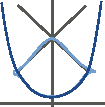
\includegraphics{figures/6_4Chaos.pdf}
            \caption{}
            \label{}
        \end{figure}
        \begin{table}[H]
            \centering
            \begin{tabular}{c|c|c}
                \textbf{Zusammenfassung:} & \textcolor{red}{Elektronen} & \textcolor{blue}{Löcher} \\ \hline \hline
                Ladung & -e & e \\
                eff. Masse & $m_e^* < 0$ & $m_h^* = - m_e^* > 0$ \\
                Wellenvektor & $\textbf{k}_e$ & $\textbf{k}_h = - \textbf{k}_e$ \\
                Energie & $E_e(\textbf{k}_e)$ & $E_h = - E_e(-\textbf{k}_e)$ \\
                Geschwindigkeit & $\textbf{v}_e(\textbf{k}_e)$ & $ \textbf{v}_h = \textbf{v}_e (- \textbf{k}_e)$ \\
                Spin & $\uparrow \downarrow$ & $ \downarrow \uparrow $
            \end{tabular}
        \end{table}
\end{itemize}



\subsection{Ladungstransport in Metallen} \label{sec:6_3}
\begin{itemize}
    \item[(a)] \textbf{Drude-Modell:}
    Ann.: Elektronen sind freie, klassische Teilchen
    \begin{itemize}
        \item[$\rightsquigarrow$] Bewegung mit therm. Geschwindigkeit $\textbf{v}_th$
        \item[$\rightsquigarrow$] Stöße mit Atomrümpfen in mittlerer Stoßzeit $\tau$
        \item[$\rightsquigarrow$] äußeres Feld \textbf{E} (oder \textbf{B}) 
        \item[$\rightsquigarrow$] Driftgeschwindigkeit $\textbf{v}_D = \textbf{v} - \textbf{v}_{th}$
    \end{itemize}
    BGL: $$ m^* \frac{\mathrm{d} \textbf{v}}{\mathrm{d}t} = - e \textbf{E} - m^* \frac{\textbf{v}_D}{\tau}$$ mit Driftgeschwindigkeit $\textbf{v}_D$ und der mittleren Stoßzeit $\tau$. Für Elektronen im Metall ist $m = m^*$\\
    Stationärer Zustand: $\frac{\mathrm{d} \textbf{v}}{\mathrm{d}t} = 0$
    $$\textbf{v}_D = - \frac{e \tau}{m} \cdot \textbf{E} = - \mu \textbf{E}$$ mit Beweglichkeit:
    \begin{center}
        \fbox{$\mu := \frac{e \tau}{m}$}\\
    \end{center}
    Stromdichte:
    \begin{align*}
        \textbf{j} = -e \cdot n \cdot \textbf{v}_D = \frac{n e^2 \tau}{m} \cdot \textbf{E} = n \cdot e \cdot \mu \cdot \textbf{E}
    \end{align*}
    mit elektrischer Leitfähigkeit \fbox{$\sigma = \frac{n e^2 \tau}{m} = n e \mu$}\\
    $\textbf{j} = \sigma \textbf{E}$ ist die mikroskopische Form des Ohmschen Gesetzes.\\
    $\sigma$ durch Materialparameter bestimmt. Für typische Metalle: $n \sim 10^{30}$ m$^{-3}$, $\tau \sim 10^{-14}$ s, damit $\sigma \sim 10^8 \frac{1}{\Omega \text{m}}$.\\
    z.B. bei 300 K:
    \begin{table}[H]
        \centering
        \begin{tabular}{r l}
            Ag: & $\sigma$ = \SI{6.1}{\cdot 10^7 (\Omega m)^{-1}}\\
            Cu: & $\sigma$ = \SI{5.8}{\cdot 10^7 (\Omega m)^{-1}}\\
            Au: & $\sigma$ = \SI{4.5}{\cdot 10^7 (\Omega m)^{-1}}
        \end{tabular}
    \end{table}

    Erfolge des Drude-Modells:
    \begin{itemize}
        \item DC Leitfähigkeit (Ohmsches Gesetz, siehe oben), AC Leitfähigkeit ($\sigma = \frac{n e^2 \tau}{m} \cdot \frac{1}{1-i\omega \tau}$)
        \item Hall-Effekt (B-Feld)
        \item Wiedemann-Frantz-Gesetz:\\
        Zusammenhang zwischen elektrischer und thermischer Leitfähigkeit $$\frac{K}{\sigma} = \frac{\pi^2}{3} \left(\frac{k_B}{e}\right)^2 \cdot T$$
        $\rightsquigarrow$ gute elektrische Leiter $\leftrightarrow$ gute Wärmeleiter
    \end{itemize}
    Problem (?): Im Drude Modell werden alle Leitungselektronen beschleunigt \& gestreut. Widerspruch zu Fermi-Dirac-Verteilungsfunktion

\item[(b)] \textbf{Sommerfeld Modell} ($\rightsquigarrow$ vgl. auch Kap. \ref{kap:5_1})
\begin{itemize}
    \item[Ann.:] Elektronen sind Quasiteilchen, quantenmechanische Teilchen $\rightarrow$ SGL, Pauli-Prinzip
    \item[$\rightarrow$] einfache Metalle (Alkali- und Edelmetalle)
    \item[$\rightarrow$] $\sim$ halb gefülltes Leitungsband
    \item[$\rightarrow$] Fermi-Fläche ist $\approx$ Fermi-Kugel
\end{itemize}
BGL unter E-Feld:
\begin{align*}
    \hbar \dot{\textbf{k}} = \dot{\textbf{F}} = - e \textbf{E} \quad \rightarrow \quad \text{\fbox{$\delta k = - \frac{e \textbf{E} \delta t}{\hbar}$}}
\end{align*}
Interpretation:
\begin{itemize}
    \item Bei \textbf{E} = 0 ist die Fermi-Kugel um \textbf{k} = 0 zentriert.
    \item Für \textbf{E} $\neq$ 0 verschiebt sich die gesamte Fermi-Kugel um $\delta$\textbf{k}.
\end{itemize}
% \begin{figure}[H]
%     \centering
%     \includegraphics[width=0.8\textwidth]{figures/5_fkugel_verschiebung.png}
%     \caption{}
%     \label{fig:5_fkugel_verschiebung.png}
% \end{figure}
\begin{itemize}
    \item Umverteilung von Elektronen von \textcolor{green}{///} nach \textcolor{blue}{///} durch Streuung
    \item Stationärer Zustand: Verschiebung der Fermilänge durch Relaxationszeit $\tau$ gegeben.
    \begin{center}
        \fbox{$\delta \textbf{k} = \frac{-e \textbf{E} \tau}{\hbar}$}
    \end{center}
    \item $\delta k / k_F \approx 10^{-7}$, d.h. $f-f_0 \neq 0$ nur in der Nähe von $k_F$
    \item Nur Elektronen in halbmondförmigen Bereichen tragen zur Leitfähigkeit bei.\\
    Kein Widerspruch zum Drude-Modell, denn:
    \begin{align*}
        \textbf{j}_{D = Drude} &= - e \cdot n \cdot \textbf{v}_D = + \frac{e \tau \textbf{E}}{m} \cdot \frac{\hbar \textbf{k}_F}{\hbar \textbf{k}_F}\\
        &= -e \cdot \tilde{n}\cdot \textbf{v}_F \qquad \text{mit} \quad \tilde{n} = n \cdot \frac{\delta \textbf{k}}{\textbf{k}_F}\\
        &= \textbf{j}_{S = Sommerfeld}
    \end{align*}
    $\tilde{n}$ gilt als an der Verschiebung beteiligte Ladungsträgerdichte.
\end{itemize}

Erfolge des Sommerfeld-Modells: Leitfähigkeit, Wiedemann-Frantz-Gesetz

\end{itemize}

\section{Halbleiter} \label{kap:7}
Folien: \textit{2019-20\_FK\_Kap7.pdf}

\end{document}
